\documentclass[11pt]{cmuthesis}
% \documentclass[11pt, draft]{cmuthesis}

\sisetup{
  round-mode          = places, % Rounds numbers
  round-precision     = 2, % to 2 places
}
%> ---------------------------------------------------------------------------------------------------------------
%> Line spacing. Neither EPP nor College of Engineering mandates either single- or double-spacing.
%> The default is to use single-spacing. If you want to use one-and-a-half or double-spacing,
%> uncomment ONE the following lines.
\onehalfspacing
\doublespacing

%> ---------------------------------------------------------------------------------------------------------------
%> Put here all those things that are common to the whole thesis. It makes sense
%> to put names that may change, or some numbers that you repeat many times but
%> are amenable to change; e.g., the number of participants in your studies.
\newcommand{\TotalParticipantsStudyOne}[0]{573}
\newcommand{\TotalParticipantsStudyTwo}[0]{982}


\begin{document}
%> First pages. Do not modify.
\frontmatter
\pagestyle{plain}

%> ------------------------------------------------------------------------------
%> This file contains most of the definitions you will need to put together
%> your thesis. All requirements were taken from the sources below:
%> http://www.cit.cmu.edu/current_students/graduates/thesis_dissertation_policies.html
%> https://www.epp.cmu.edu/graduate/thesis_format_guide.html
%> ------------------------------------------------------------------------------

%> Your title goes here.
\title{Development of a Global Data Center Infrastructure Systems Model bound by the System’s End to End Life Cycle}

%> Your own name goes here.
\author{Eric Kumar}
\affiliation{School of Architecture}

%> Put your previous degrees here.
\bsdegree{Mechanical Engineering, Sacramento State University}
\msdegree{Fire Protection Engineering Engineering, Cal Poly San Luis Obispo}

%> Put the month you will be graduating here, NOT the month in which you
%> actually finished the thesis. The only admissible months here are May,
%> August and December.
\Month{September}

%> Year in which you graduated (or plan to graduate).
\Year{2020}



%> Copyright notice. This may be whatever you want. My personal choice is to
%> make it as widely accessible as possible :)
\permission{\textit{Some rights reserved.} Except where indicated, this work
is licensed under a Creative Commons Attribution 3.0 United States License. 
Please see \smallurl{http://creativecommons.org/licenses/by/3.0/us/} for
details.}

%> Keywords.
\keywords{data centers, building energy models, network traffic, sustainable engineering, green design.}
\maketitle

%> ------------------------------------------------------------------------------
%> Abstract. Mandatory and very important. Keep it under 350 words.
%> ------------------------------------------------------------------------------
% \begin{abstract}
% This work is dedicated to \\
% ... my daughter, to whom it shows that anything is possible given the dedication. \\
% ... my parents, who left paradise to give me an opportunity that my ancestors never had. \\
% ... my wife, who has shared my sacrifices and paid  the opportunity costs for it's path.
% \end{abstract}

\section{Abstract}

Data centers (DCs) are critical for modern society. They house information technology (IT) hardware and store data for financial institutions, social media accounts, entertainment portals, and virtual meeting forums amongst many other things. In their physical embodiment, networks of DCs are global scale systems. Within these systems, each DC’s size can be as large as a college campus and consume 100 times the amount of electrical energy every hour as residential facilities do in a day. Given their growing demand, it is extremely important to develop a global level modeling framework to help make DC design decisions that comprehensively account the total costs of ownership (TCO) of DCs inclusive of capital and operational costs..

Currently, DC design practices optimize for the power usage effective metric. However, some industry insiders have expressed that thinking of PUE in isolation may lead to inadvertently increasing the TCO for DC systems. To fill the isolated view of PUE, this research developed a prototype of an agile model that uses life cycle analysis (LCA) frameworks to quantify the holistic life cycle cost of DC systems. The developed model is composed of four software modules: 

\begin{itemize}
\item A real world internet traffic profile simulation module as a proxy for DC workloads. 
\item A module that integrates building energy simulations with dynamic DC workloads in a novel way.
\item A module that couples the building energy demands with the marginal costs of energy production.
\item A module that is composed of a hybrid of a process and economic input-output based LCA frameworks to assess the embodied costs of the global DC system.
\end{itemize}
As a framework for comprehensive TCOs, this dissertation provides DC designers two contributions. The first contribution is the affirmation that characterising DC costs requires a modular approach. This modular approach is at least three tiered, where the first tier must characterise the infrastructure in terms of materials and operational processes. In the second tier, the model must be aware of the workload interactions within the system. The third and final tier allows the application of objective models to quantify various forms of costs associated with DCs. Using this three tiered approach a demonstration for the total carbon footprint of a set of hypothetical internet service is demonstrated.   

The second contribution is shown through the coupling of the network driven workloads and the building energy simulations. The research proves the feasibility of inverse cooling plant controls; where the chiller operational point can be kept at a constant load by varying the IT power loads for batch tasks. Opportunistic varying of batch tasks allows over-subscription of workloads when the cooling plant is at conventional part loads.

%> ------------------------------------------------------------------------------
%> Dedication. Optional. This is whatever you want.
%> ------------------------------------------------------------------------------
\begin{dedication}
This work is dedicated to \\
... my daughter, to whom it shows that anything is possible given the dedication. \\
... my parents, who left paradise to give me an opportunity that my ancestors never had. \\
... my wife, who has shared my sacrifices and paid  the opportunity costs along my path.
\end{dedication}


%> ------------------------------------------------------------------------------
%> Acknowledgements. Mandatory. At the very least you should acknowledge
%> your committee and your funding sources.
%> ------------------------------------------------------------------------------
\begin{acknowledgments}
TBD
\end{acknowledgments}


\tableofcontents
\listoffigures
\listoftables
\mainmatter

%> Configuration of the headers
\pagestyle{fancy}
\lhead[\footnotesize\emph{\chaptername\ \thechapter. \leftmark}]{}
\rhead[]{\footnotesize\emph{\thesection. \rightmark}}


%> Content. This section contains references to the chapters in your thesis.
%> Modify as you please.
\chapter{Wide Area Network Based Data Center Energy Simulations for Internet Services}
\label{chp:traffic}

\section{Chapter Abstract}
    Data centers are a critical component of modern day economies and social lives of people all around the world. In many aspects society’s dependency on internet services enabled by data centers is still increasing; the COVID-19 stay in place orders are a current example of unprecedented growth rates for many internet services. With the increased dependency on data centers, there is a concern about their environmental impacts across at the globe scale. To reason about the environmental footprint of these globally spanning system requires a new approach to model building energy use of facilities within these systems. This paper demonstrates a top down process that leverages publicly available network traffic data for a globally distributed internet site to model it’s power demand, using Wikipedia as the model internet site. The traffic provides an indication of the building loads that the data center infrastructure must support.  
    
    This chapter demonstrates a method to geographically correlate five data centers with the incoming visits from a global user base using a minimum cost function. The correlations are further extended to provide a forecast of the traffic. The contribution of this research is two-fold. First, it presents a method for a top down assessment of network traffic that can characterize the information technology loads in building energy models. Second, the traffic forecast allows data center operators and designers to model future demands of the building infrastructure systems and perform scenario models based on the projected traffic. 

\section{Introduction}

    Data centers are ubiquitous in today’s society. Consumers of data center enabled web services expect high availability of their functionality and access to their data on a continual basis. These expectations are met with software architectures that provide strongly consistent views of the data regardless of location and in the presence of physical systems failures. In terms of specific failure domains, network failures can be the most catastrophic. For example, an outage of a network link connecting a data center can lead to all physical resources in it to become inaccessible from the outside. With these expectations, the dependencies of internet data centers and their communications network during failures is clearly apparent.
    
    Data center utilities (such as mechanical cooling resources and power distribution resources) and their network connections are not only coupled in failure scenarios described above, but they are also in lock-step with each other through normal operations. This coupling is also easy to reason about; as internet data centers don’t generate workloads hermetically. The workload demands for data centers come from remote consumers (user facing traffic) and other adjacent data centers (back-end traffic). Both forms of incoming traffic instantiate computational and storage processes on the IT hardware, which in turn are powered and cooled by district scale distribution plants.
    
    In the current generation of data centers, the building utility systems demand less than 10\% of the total energy delivered to the site \cite{Shehabi16}. The balance of the power of these new data centers is consumed by the information technology (IT) equipment. With this disproportionate allocation of energy, it is clear that the total energy use in data centers is more sensitive to ITE loads than the facilities systems. Yet the building systems still receive the most attention in the design and facilities operations phase of the buildings. Others have also pointed out similar gaps data center building energy models \cite{Beatty15}. 
    
    To provide an intuition of data center networks, Figure~\ref{net_diag} shows a generalized depiction their topology. At the top are the internet service provider (ISP) networks are shown as clouds because the physical paths of these systems are managed by the global ISPs and they are typically out of control of data center operators. Data center operator’s depend on the ISPs for connecting their facilities through private wide area networks (WAN). The pink lines indicate these wide area connections that traverse over ISP networks. The magenta links connect global WANs data center metropolitan, which typically are responsible for the last miles of network distribution. Within the metropolitan area, their maybe one or more data center sites, only two are shown for clarity in the figure. 
    
    \begin{figure}[h]
\centering
    \includegraphics[scale=0.2]{traffic_profile/images/net_diag.png}
    \caption[Network Diagram]{Generic Data Center Network Topology.}
\label{net_diag}
\end{figure}

    
    To motivate business incentives  for  a  more  integrated  IT  and  building model, the  data  center construction spending is estimated to be \$89 billion by 2027, nearly doubling the spend seen in 2018 \cite{dcmarket19}. At the core,the demands for data centers is driven by the expected consumer traffic to its services. With this much value at stake, capital and operational decisions must be based on robust system level models that couple IT traffic and data center designs.
    
\section{Background}
    EnergyPlus, the US Department of Energy’s building energy modeling software has supported data center model since release 8.3. [4]. EnergyPlus modeling engine allows for IT equipment load schedules to be explicitly modeled in it. Today, EnergyPlus comes with three example data center models, in the form of IDF files. These IDFs provide a template that energy analysts can extend and augment to represent their specific data center designs. These default templates are hermetic and lack coordination with the dynamic IT loads. However, there are supplemental software applications that allow external software to integrate with EnergyPlus yielding a robust feedback loop. Building Control Virtual test bed (BCVTB) is one such application \cite{EnergyPlus8.3}. 
    
    \begin{figure}[h]
\centering
    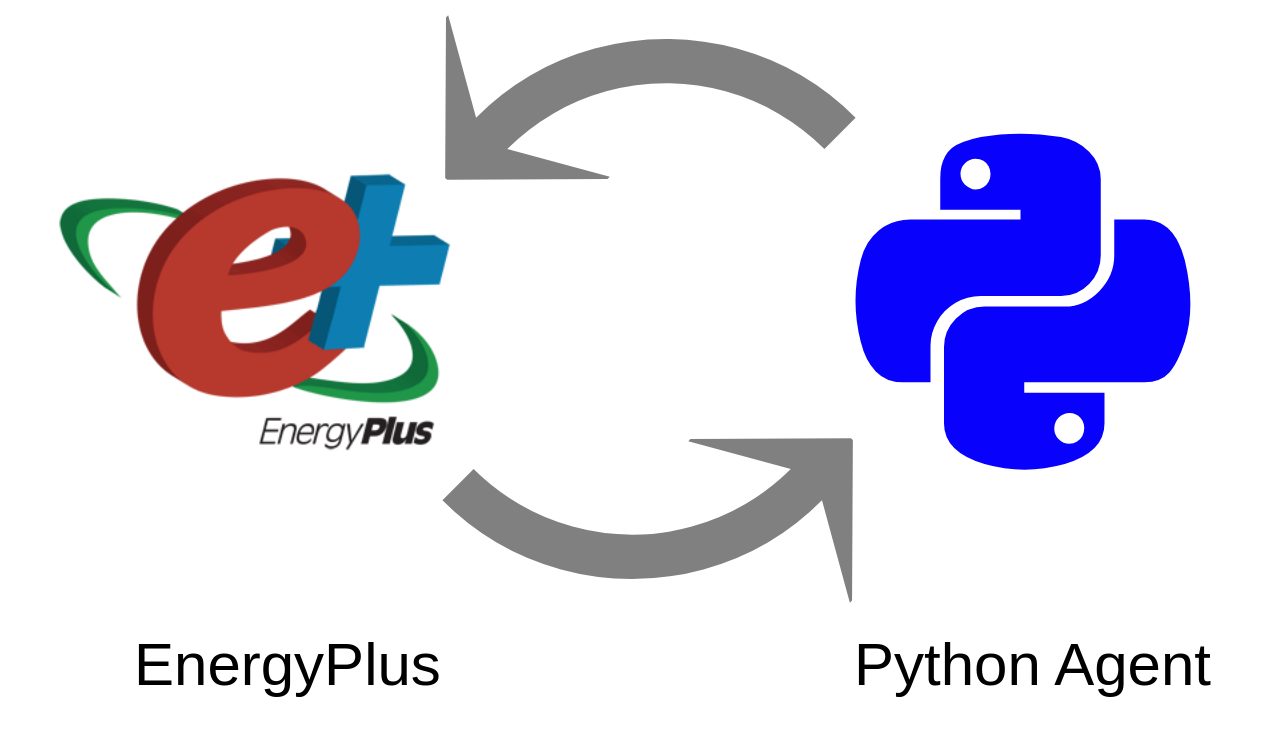
\includegraphics[scale=0.15]{traffic_profile/images/agent_bem.png}
    \caption[Software Agent and BEM Interaction]{General process flow between EnergyPlus and internet traffic simulation.  .}
\label{agent_bem}
\end{figure}
    
    Wei demonstrates the use of BCVBT in \cite{wei17} for modeling a mixed used facility and has a data center collocated with occupied spaces. Zhang demonstrated the use of BCVBT for control an educational building \cite{zhang19}. Zhang published their Python code base to allow others to replicate their work. Functionally, BCVTB creates an interactive process loop with EnergyPlus allowing the Python program to be aware of EnergyPlus simulations at every simulation time step. Figure 2 illustrates this interactive loop between EnergyPlus and Python. Next, background about wide area network from an internet service perspective is provided. 
    
    Wide area networks serve as the backbone for many internet applications that operate across regionally distributed data centers. The traffic on the inter data center links are segregated into three classes; interactive, large file transfers, and background. Linkedin’s experience with these three classes of traffic is document well by Zhuang \cite{zhuang15}. Interactive traffic consists of blocking operations; where the sequential byte level transactions are required to keep things proceeding. Large file transfers entail transmission of requested resources by some deadline. Background traffic are workloads that opportunistically send traffic and preempting them does not expose the system to any idempotent side effects. Database communications traffic typically consists of workloads that are bound by deadlines and are also pseudo-interactive. These three classes of traffic can either be user facing or back-end. Microsoft and Google have both published their experiences in designing and operating these massive global networks \cite{hong13, sushant13}.  

\section{Methodology} 
    In this section the methods for synthesizing network traffic to correlate it with data center workloads is described. There are four step-wise methods that ultimately yield results that are usable for building energy modeling. These sub-sections first describe the service level data-set that is used throughout this article. Then the service level information is abstracted to indicate network bandwidth, which in turn is correlated with power in the third sub-section. The final method discussed shows a method to scale historical service demands into projection of future loads for data centers.  
    
    \begin{figure}[!htn]
  \subfloat[Mean Value of Page Views]
  {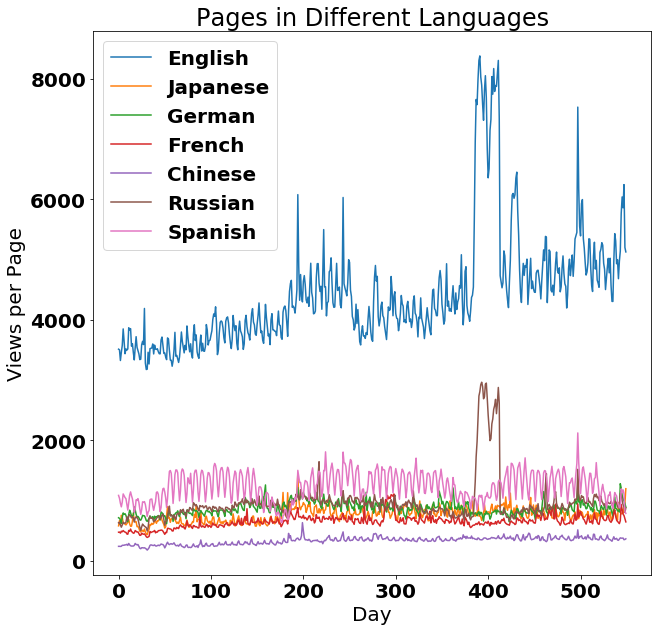
\includegraphics[width=0.5\textwidth]{traffic_profile/images/mean.png}\label{mean}}
  \hfill
  \subfloat[$95^{th}$ Quantile Value of Page Views] 
  {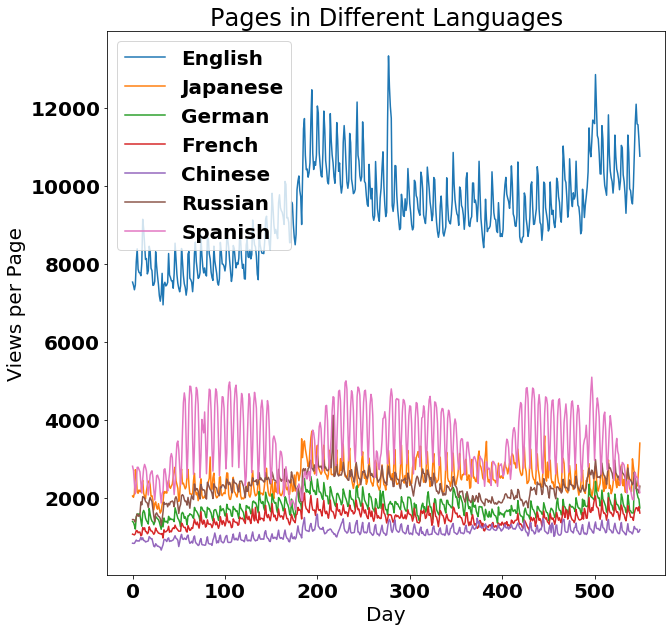
\includegraphics[width=0.5\textwidth]{traffic_profile/images/quantile95_use.png}\label{95thquantile}}
  \caption[Page Views by Language]{Pages Views for Each Language}
\end{figure}

    Traffic to 145,063 Wikipedia Pages for 803 days from July 2015 through September 2017 is used to demonstrate a top-down WAN model for global services. The data is used to train and test the models developed in this section. The training set is partitioned to be inclusive of traffic from July 2015 to December 2016. The remaining data is used to test accuracy of the models. All pages are segregated into 7 different languages; namely English, Japanese, German, French, Chinese, Russian, and Spanish. The mean volume of visits per language is shown in \ref{mean} and the 95th quantile is shown in \ref{95thquantile}.  
    
    The curves in Figure 3 are indicative of the distribution of visits for each of the seven languages found in the data set.  For example, the 95th quantile is indicating that 95 percent of the pages in the language were visited as noted on the y-axis on the day number noted on the x-axis. While the average curves indicate that on average, the number pages in the language are visited as noted in the y-axis on the corresponding day count. Both of these curves can be used in the design phase of the data center buildings, with the 95 quantile determining the capacity and the average values supporting operational models. In this article, the average value is used as the indicator of the operational network model. 
    
    \definecolor{chinese}{rgb}{0, 1, 0} %chinese 
\definecolor{english}{rgb}{0, 0, 1}%english 
\definecolor{french}{rgb}{.8, 0, 0}%french 
\definecolor{german}{rgb}{.5, .5, .5}%german 
\definecolor{japanese}{rgb}{0, 0, .5}%japanese 
\definecolor{russian}{rgb}{0, .5, 0}%russian 
\definecolor{spanish}{rgb}{0, .25, .5}%spanish 


\begin{figure}[h]
\centering

        \begin{tikzpicture}
        \begin{scope}[xshift=1.5cm]
            \node[anchor=south west,inner sep=0] (image) at (0,0)
            {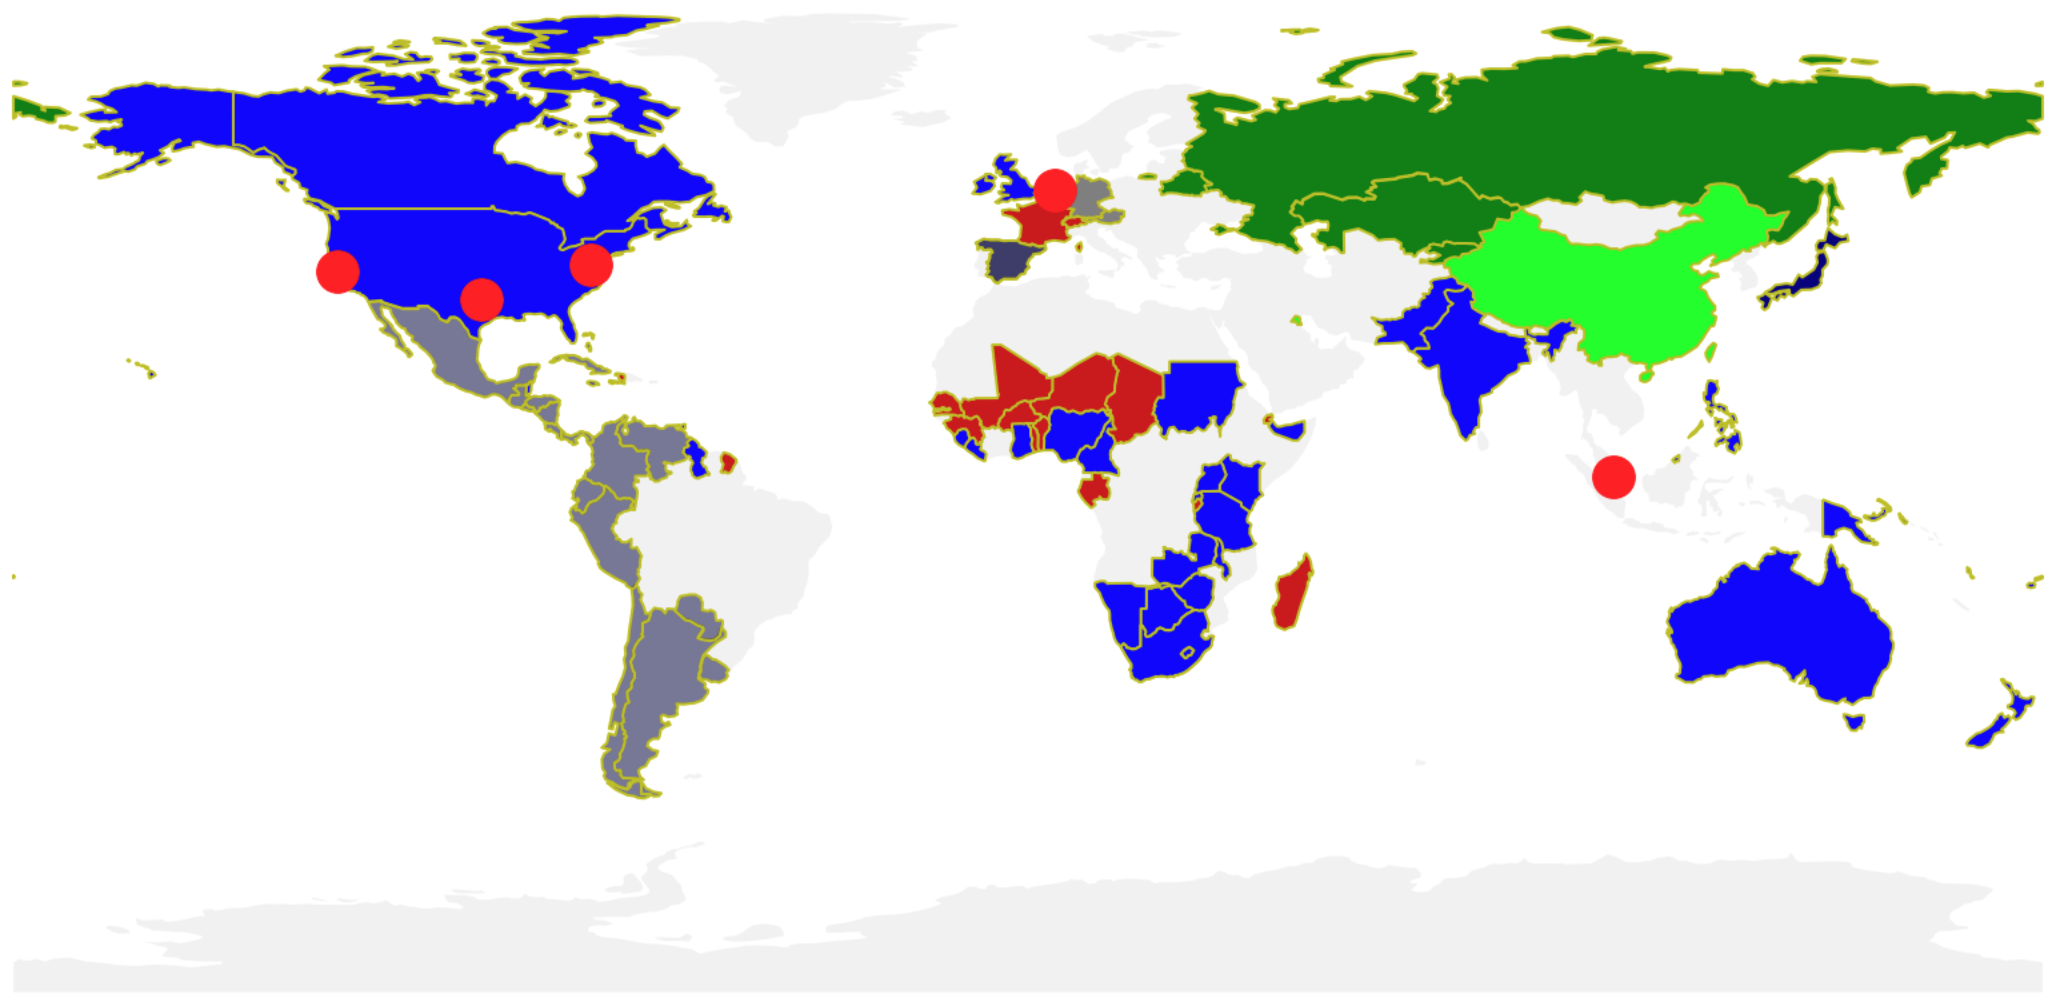
\includegraphics[width=1\textwidth]{embodied_cost_model/images/world_language_map_3.png}};
        \end{scope}
        
        \begin{scope}[xshift=1.0cm]
            \node [anchor=center] (chinese) at (2,-.6) {\small{Chinese}};
            \filldraw[outer color=chinese, inner color=chinese] (1.8,-.4) rectangle (2.2,0); % chinese
            
            \node [anchor=center] (english) at (4,-.6) {\small{English}};
            \filldraw[outer color=english, inner color=english] (3.8,-.4) rectangle (4.2,0); % english
            
            \node [anchor=center] (french) at (6,-.6) {\small{French}};
            \filldraw[outer color=french, inner color=french] (5.8,-.4) rectangle (6.2,0); % french
            
            \node [anchor=center] (german) at (8,-.6) {\small{German}};
            \filldraw[outer color=german, inner color=german] (7.8,-.4) rectangle (8.2,0); % german
            
            \node [anchor=center] (japanese) at (10,-.6) {\small{Japanese}};
            \filldraw[outer color=japanese, inner color=japanese] (9.8,-.4) rectangle (10.2,0); % japanese
            
            \node [anchor=center] (russian) at (12,-.6) {\small{Russian}};
            \filldraw[outer color=russian, inner color=russian] (11.8,-.4) rectangle (12.2,0); % russian
            
            \node [anchor=center] (spanish) at (14,-.6) {\small{Spanish}};
            \filldraw[outer color=spanish, inner color=spanish] (13.8,-.4) rectangle (14.2,0); % spanish
            
            \node [anchor=center] (dc_location) at (9,-1.1) {\small{Data Center Locations}};
            \filldraw[red] (7,-1.1) circle (4pt); 
            
            \end{scope}
            
        \end{tikzpicture}

\caption[Source country of language and DC locations]{Source country of language and DC locations map.}
\label{image:world_language_map}
\end{figure}
    
    After segregation of the pages by language and dropping pages without language indicators, the languages are mapped to countries in which they are the official language. Figure 4 shows the mapping of languages to their respective countries by color groups; English (blue), Japanese (navy blue), German (gray), French (red), Chinese (light green), Russian (forest green), and Spanish (cyan). Red markers indicate the locations of Wikipedia data centers from around the world as listed in Table~\ref{language_to_dc}.
    
    
\begin{table}[h!]
    \begin{center}
    \scalebox{0.8}{
    \pgfplotstabletypeset[
        col sep=comma,
        string type,
        columns/DC/.style={column name=DC, column type={|l}},
        columns/en/.style={column name=English, column type={|c}},
        columns/ja/.style={column name=Japanese, column type={|c}},
        columns/de/.style={column name=German, column type={|c}},
        columns/fr/.style={column name=French, column type={|c}},
        columns/zh/.style={column name=Chinese, column type={|c}},
        columns/ru/.style={column name=French, column type={|c}},
        columns/es/.style={column name=Spanish, column type={|c}},
        columns/total/.style={column name=Total, column type={|c|}},
        every head row/.style={before row=\hline,after row=\hline},
        every last row/.style={after row=\hline},
        ]{traffic_profile/content/data/Language_to_DC.csv}}
    \end{center}
    \caption[Languages to Ingress Sites]{Languages to Ingress Sites}
    \label{language_to_dc}
\end{table}


    
    Throughout this research these Wikipedia data centers are used to the model the network based on publicly available information. Several additional assumptions are made in regard to the attributes of the system that are not in the public domain. Furthermore, some of the system complexity is reduced for brevity. For example, the traffic generating in a particular country is allocated with their closest ingress points as listed in Table~\ref{language_to_dc} by using a minimum distance function between the respective geographical codes. 
    
    The specific step-wise approach of mapping languages to the respective data center is shown in Table~\ref{traffic_allocation_steps}. Following these steps, Table~\ref{language_to_dc} shows that English is the most dominant language, with its traces appearing at all of Wikipedia's ingress sites while originating in 49 countries.  
    
    \begin{table}[h!]
    \begin{center}
    \scalebox{0.8}{
    \pgfplotstabletypeset[
        col sep=comma,
        string type,
        columns/Steps/.style={column name=Steps, column type={l}},
        columns/Description/.style={column name=Description, column type={l}},
        every head row/.style={before row=\hline,after row=\hline},
        every last row/.style={after row=\hline},
        ]{traffic_profile/content/data/traffic_allocation_steps.csv}}
    \end{center}
    \caption[Method for Traffic Allocation to each ingress site ]{Method for Traffic Allocation to each ingress site }
    \label{traffic_allocation_steps}
\end{table}
    
    \subsection{Scaling service demands and data center workloads}
    
    In this section, the Wikipedia traffic profiles are used to forecast future demands. Note that the traffic data is slightly modified to represent digital bits in order to demonstrate another useful insight that network traffic inherently provides. The objective here is to determine the future service demands that drive workloads at each data center. To obtain the digital payload of the pages, their contents are converted to its byte size representation. The bit size distribution of Wikipedia articles was not readily available in the public domain so an estimation method was developed for this work as follows. First, several resources were consulted to determine the page size \cite{wiki_stats, xtools}. The resulting page sizes for each of the seven languages studied in this article are noted in Table~\ref{language_to_page_size}. 
    
    \begin{table}[h!]
    \begin{center}
    \scalebox{0.8}{
    \pgfplotstabletypeset[
        col sep=comma,
        string type,
        every head row/.style={before row=\hline,after row=\hline},
        every last row/.style={after row=\hline},
        ]{traffic_profile/content/data/language_to_page_size.csv}}
    \end{center}
    \caption[Language to Page Size Classification]{Language to Page Size Classification}
    \label{language_to_page_size}
\end{table}    
    
    Now, the time series of bit-wise representation of the traffic can be analyzed to make future predictions. The time series ($t$) dependencies of a variable $X$ can generally be decomposed in trending ($T$), seasonal ($S$), and random ($R$) components, as shown in equation below \cite{zhuang15}. Specifically T exists when there is a gradual shift across time. indicates cyclic patterns, and R accounts for randomness.   
    
        \begin{equation}
        X_t = T_t + S_t + R_t
        \end{equation}
    
    In the next few paragraphs two time-series forecasting frameworks that decompose time series into these three components are discussed. First, the Auto Regressive Integrated Moving Average (ARIMA) model is presented and its implementation challenges along with its results are noted. Second, as alternate to ARIMA, Prophet another time-series modeling tool is implemented and its details along with its results are presented. 
    
    \emph{ARIMA Model}: First, time-series analysis is performed using the Auto Regressive Integrated Moving Average (ARIMA) model. The auto regression component leverages the dependencies between an observation and some lagged time step. The integration component differentiates the raw observations from preceding time steps to make the series stationary. The moving average component quantifies the dependency between observations and residual errors with a moving average model applied to lagged observations. Each of the three components are specified as a model input parameter in the form ARIMA(p, d, q). The parameter p indicates the lag order, d indicates the degree of difference (i.e. the number times raw observations are differenced), and q indicates the size of the moving window (the moving average). 
    
    The ARIMA model has been used effectively in previous literature to forecast 21 days of network traffic with 42 days of past trends [8]. This research extends the forecast out to 9 months. Figure 5’s legend indicates the use of combination of ARIMA(2,1,2) and ARIMA(1,2,4) as parametric arguments to the ARIMA module. The generated estimate is based on 550 historical records for each site and forecasts the traffic profile 250 days beyond the training data cutoff date. Figure 5 shows that the ARIMA predictions are heavily influenced by the trend near the training cutoff period. As shown, the ARIMA models appear to capture weekly seasonality well but fail accurately capture longer seasonality periods; given the time range of the our dataset with the parametric used in this work. Nonetheless, ARIMA models are capable of including seasonal covariates to improve sensitivity to longer cyclic periods, but the attempts to model with Seasonal Auto-ARIMA led to extremely long fitting times at best or the models didn't converge on a solution. 
    
    \begin{figure}[h]
\centering
    \includegraphics[scale=0.4]{traffic_profile/images/_arima.png}
    \caption[Network Diagram]{ARIMA Models: Historical trends and future projections.}
\label{arima}
\end{figure}
    
    \emph{Generalized Additive Model}: Next, a variant of the generalized additive model (GAM) was simulated with the same bit wise time series from above. The model is explained in great detail by Taylor in \cite{fbprophet}. The GAM model variant, Prophet, also has a decomposable time series formulation similar to the time series dependence equation from above. However, Prophet is supplemented with a term that accounts for holidays that occur at idiosyncratic  intervals. 
    
    Prophet has a novel concept that deals with trends in forecast uncertainty, in that it uses a Laplace transform to randomly distribute future change points in the trend based on past data. This can be seen by how closely the forecasts, blue lines track the historical data, black dots in Figures~\ref{DFW}, \ref{AMS}, \ref{SFO}, \ref{SIN} and the actual forecast based on the test data (magenta lines in figure). The change point parameter is set to 0.3 and the yearly seasonality parameter is set to True for these simulations. The forecast extends beyond the test data range which shows the that the cone of uncertainty increases as the forecast is extended out further indicated by the light blue curves. 
    
    
    
    \begin{figure}[!htn]
  \subfloat[Carrollton (DFW)]
      {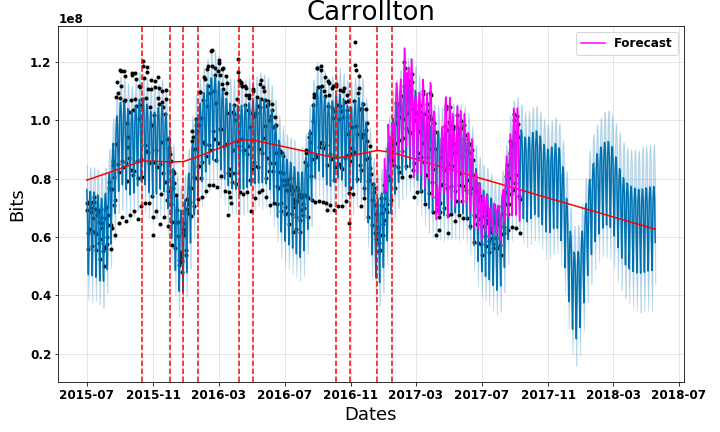
\includegraphics[width=0.5\textwidth]{traffic_profile/images/Carrollton_prophet.png}
      \label{DFW}}
  \hfill
  \subfloat[Haarlem (AMS)]
      {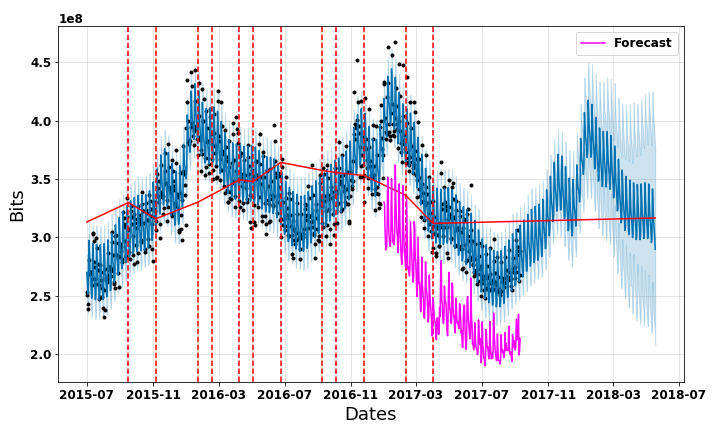
\includegraphics[width=0.5\textwidth]{traffic_profile/images/Haarlem_prophet.png}
      \label{AMS}}
  \hfill
  \subfloat[San Francisco (SFO)]
      {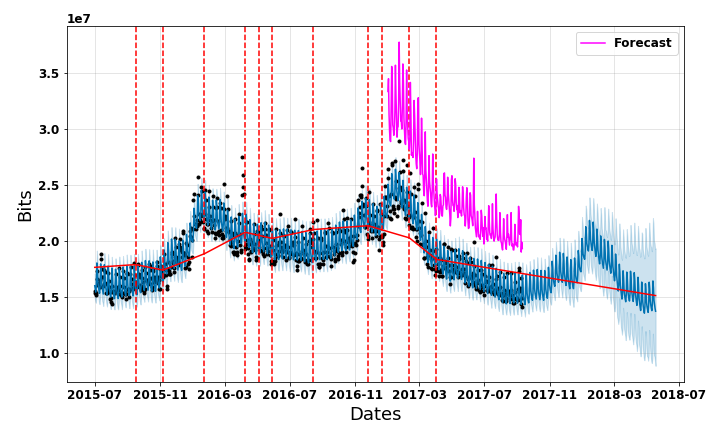
\includegraphics[width=0.5\textwidth]{traffic_profile/images/SanFrancisco_prophet.png}
      \label{SFO}}
  \hfill
  \subfloat[Singapore (SIN)]
      {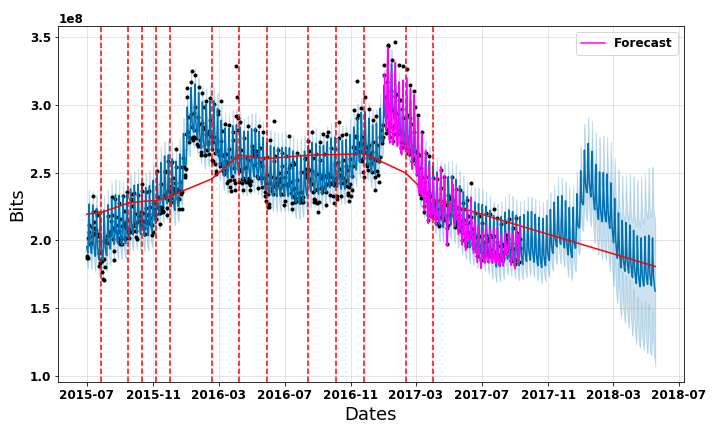
\includegraphics[width=0.5\textwidth]{traffic_profile/images/Singapore_prophet.png}
      \label{SIN}}
  \hfill
  \caption[Prophet Curves]{Prophet Historical Trends and Traffic Forecast}
\end{figure}
    % Provide a compartive table for MAPE of Arima and Prophet
    
    Table~\ref{mape} provides a comparison of the mean absolute error (MAPE) for four data center sites. The difference in error rates varies by a factor 1.72 (for SIN) and over 52 (for SFO). Overall, in comparison it is shown that the Prophet model is superior to the ARIMA model in terms of accuracy of its predication's. 
    \begin{table}[h!]
    \begin{center}
    \scalebox{0.8}{
    \pgfplotstabletypeset[
        col sep=comma,
        string type,
        every head row/.style={before row=\hline,after row=\hline},
        every last row/.style={after row=\hline},
        ]{traffic_profile/content/data/mape.csv}}
    \end{center}
    \caption[MAPE for ARIMA and Prophet Models]{Mean Absolute Percentage Error}
    \label{mape}
\end{table}
    
\section {Results}

    In this section the results from using the traffic coefficients is presented. Following the steps listed in Table~\ref{traffic_allocation_steps} yields the curves indicated in Figure \ref{ingress_hitrate_95_links}. Each curve in the figure consists of all the languages that are routed to it, truncated to the . 
    
    To reason about these curves, recollect the distribution of the languages at each data center form Figure 1. For example, the curve for San Francisco (SFO) in Figure 7 is nearly 100 times smaller than the curve for the Haarlem (AMS) site. This is due to only four countries being routed to San Francisco, whereas Haarlem has traffic routed from 38 countries. 
    
    Figure 8 shows the resulting CPU power profiles when using traffic coefficients in EnergyPlus simulations. The average page view values are used as indicated in Figure 3A for the English language. The details of the EnergyPlus configuration are provided by Kumar in [14]. Since the English language is the dominate language at the San Francisco site nearly all of the CPU resources at the site are dedicated to it. The constant load profile for San Francisco is constant in the figure and can be attributed to the nearly flat curve for San Francisco shown in Figure 7. 
    
    \begin{figure}[h]
\centering
    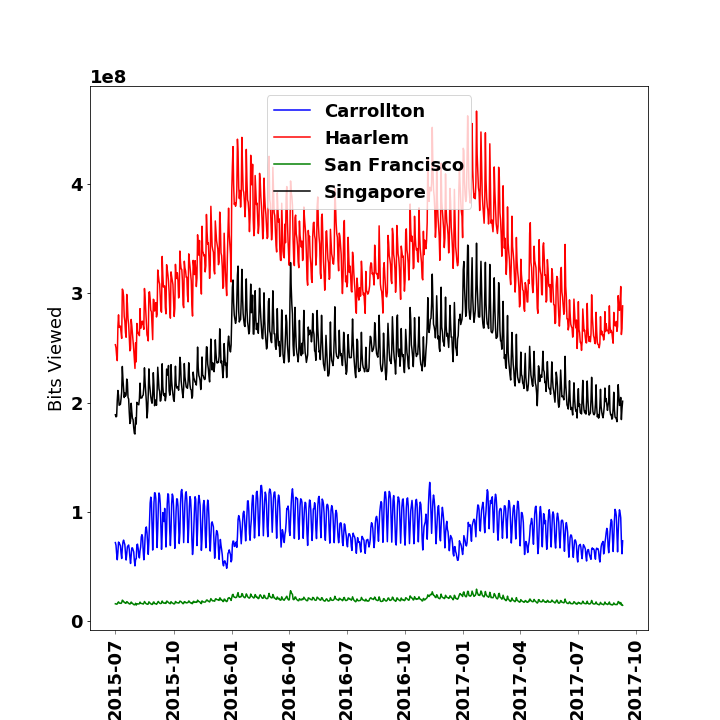
\includegraphics[scale=0.35]{traffic_profile/images/ingress_hitrate_95_links.png}
    \caption[Total Traffic to Each Site after mapping]{Total Traffic to Each Site after mapping.}
\label{ingress_hitrate_95_links}
\end{figure}
% \chapter{Building Energy Model of DCs}
% \label{chp:bem}

% For the conference, need \citepp{}, otherwise for dissertation replace with \citep{}

\section*{Abstract}	% Section headings need to be upper and lower case.
% -------------------------------------------------------------------------------------------------------------------------------

\addtocounter{section}{1}

% Relate to title
% Towards Energy Simulations for Proportionally Designed and Controlled Data Centers

Expressing site-specific load profiles and hardware specifications that reflect the information technology (IT) processes inside data centers have always been a challenge to do either benchmarks of building energy performance or predictive controls. As a substitute, data center building models usually assume naive hour-day-week schedules that don't align simulated operations with the weather profiles. 
This paper demonstrates a method towards using more representative load profiles in data center energy models by deriving the profiles based on global usage patterns of an internet platform. It is the first attempt to illustrate the coupling of an external signal with EnergyPlus as an indicator of IT load in a data center. 

% -------------------------------------------------------------------------------------------------------------------------------
\section{Introduction}
% -------------------------------------------------------------------------------------------------------------------------------

\added{This paper describes a data center (DC) building energy simulation framework. The framework is based on EnergyPlus as the physical model of the building operations and an externally implemented network traffic schedule as an indicator of the IT load. Namely, the target applications for these frameworks are the hyper-scale facilities that house global services such as social networks and search engines. For this class of facilities, the significance of network traffic to DC operations is exemplified by the sudden change in peoples internet usage behaviors due to the COVID-19 pandemic. Through the pandemic, DCs across the globe have seen a disruptive shift in user traffic patterns that were not known just weeks prior to the first stay-in-place orders. Given this timely example, it is imperative that DC operators be able to simulate their facilities to verify that their infrastructure can handle these types of shifts in traffic. However, presently there is a lack of publicly available information about how to build such simulations. 


The contribution of this work is two-fold. First, it provides a demonstration for characterizing data centers and IT equipment in EnergyPlus. Second, by deriving the workload profile from network traffic, this work provides a perspective for reasoning about temporal profiles of the workloads that hyper-scale data centers must support.}

\deleted{DCs are the backbone of today's internet based economy. From an energy perspective, in the U.S DCs consume around 2\% of the total energy produced, with 10 times or more power density then conventional office buildings. Through the COVID-19 pandemic, DCs across the globe have seen a disruptive shift in traffic and workload patterns. Given this timely example, it is warranted that DC operators be able to simulate their facilities to verify that their infrastructure can handle these types of shifts in traffic. This research proposes that dynamic computational workloads of DCs can be sufficiently and accurately characterized with current building energy modeling tools to allow such simulations.

The methodology presented in this article couples a network model indicative of internet traffic with the building power load profiles. The effectiveness of such a model is demonstrated by extending the model to five DCs dispersed globally and comparing their results. The framework can be used by architects and designers to assess building energy models of DCs and to provide an indicator of opportunistic thermal headroom during non-design day conditions.}

\deleted{In 2020 U.S DCs are projected to consume 73 billion kWh \citep{Shehabi16}. This value is significantly curtailed from the trends documented in a 2007 Report to Congress \citep{koomey07}. The report provided evidence of unsustainable energy demands by DCs as the industry expanded, based-on the industry's growth observed from the early 2000’s. Koomey's report was a medium that spread awareness of the problem. Since then various opportunities for energy reduction have been identified and implemented by IT equipment and facility systems architects.

Two specific engineering choices have had profound benefits towards DC energy efficiency. First, proportional power and thermal control of DC components is now enabled across all dimensional scales. An example of a millimeter scale proportional control is of central processing units (CPU) with dynamic frequency voltage scaling (DFVS) \citep{osullivan15}, \citep{barroso18}, \citep{joshi12}.

To appreciate the DFVS’ correlation across the distinct technical domains of computer systems and buildings it should be noted that legacy hardware operations did not proportionally utilize power or cooling with their IT workloads. Most intuitively, this meant that an IT device consumed nearly the same amount of power whether it was idle or being 100\% utilized. The latest generation of IT equipment have much better proportional control enabled by variable fan speeds, variable power draw, and variable heat dissipation resulting from workload dependent power draw enabled with DFVS.  

Second, power and thermal constraints have been relaxed compared to legacy practices. As an example, led by hyper-scale early adopters like Facebook,dual conversion power typologies are now being replaced with bypass systems \citep{Park15}. The removal of dual conversion power systems not only saves capital costs associated with complex uninterruptible power distributions, but it also saves operational expense by requiring power rectification at the IT point of connection only. 

Omission of dual conversion power distribution systems is one example that has been enabled by deep integration across IT and building systems power architectures. Another example is the collaboration between thermal architects of IT and buildings that led to the expansion of the operational environment's thermal psychometric window for IT equipment. An expanded psychrometric window increases the opportunity to exploit free cooling modes across various climate zones \citep{ASHRAETC9.9}. In more aggressive implementations, some DC operators have gone beyond the opportunistic use phase power usage effectiveness optimality and have discarded compressor-based equipment from their cooling plants completely. Compressor-less cooling plants offer significant capital costs savings as-well as the operational energy and maintenance costs \citep{Mulay18}.} 

\added{DCs have 10 times the power density of conventional buildings. With this density, it is essential that during the design phase designers have access to representative building energy models to size equipment and to validate jurisdictional compliance. However, these building energy models are typically put on the shelf once the facility is turned over to the operational teams. With much of the life cycle costs of a data center attributed to the use-phase, having building energy models that represent the cyber-physical dynamics of their facility can be valuable to support operational decisions too.

In this work, wide area network traffic bandwidth is demonstrated as a proxy for IT loads in data center buildings. However, any technique that characterizes a fine grain coupling between the IT workloads and the building systems would be valuable for hyper-scale DCs the running online platforms such as social media sites, search engines, or public cloud services. These platforms are typically distributed through out the world for redundancy and performance objectives for their global user base. In terms of building scale, each data center can scale beyond a hundred thousand square meters with 100s of MW of power. Even with the ever growing needs for hyper-scale data centers today, there is a lack of publicly available literature which discuss coupling building energy models with IT operations to help operators reason about actual service workloads and their building's performance} 

In the recent past, the power usage effectiveness metric ($PUE$) as defined by Equation~\ref{eq:pue} has been a key performance indicator for DC facilities architects and facilities operators. 

    \begin{equation} \label{eq:pue}
    PUE=\frac{E_{total}}{E_{IT}} 
    \end{equation}
    \begin{center}
    $E_{total}$ = Total Power Used at Facility
    
    $E_{IT}$ = Power Consumed by IT Equipment
    \end{center}
    \vspace{.2cm}
    


% \deleted{\begin{equation}\label{eq:pue}
%   PUE  = \frac{Total\; Power\; Used\; at\; Facility}{Power\; Consumed\; by\; IT\; Equipment}
% \end{equation}}

\deleted{In operations} \added{The $PUE$ is a intuitive metric to reason about. In consideration of the $PUE$, the mechanical inefficiencies and electrical distribution losses external to the IT equipment contribute to the difference between the numerator and denominator of Equation~\ref{eq:pue}}. In operations, the facilities and IT parameters change simultaneously together in a continuous sequence, lending to accurate real time evaluations. However, the continuous states of IT workloads and ambient environmental conditions makes design time PUE calculations complicated. The complications drive DC building designers to evaluate the efficiency metric, \deleted{at}\added{by averaging} discrete step-wise \added{(hour-day-week) workload values and taking the worst case values to benchmark the facility}.

\deleted{Like the PUE calculations, DC building energy models are also reasoned about through these coarse step loads. The step-wise inputs are sufficient for two things. First, for sizing equipment which must support the nominal DC capacity in any possible operational condition with the bounds of the basis of design. Second for producing energy models which are suitable for prescriptive compliance reviews; allowing  municipalities to normalize across different DCs in their jurisdiction.} 

However, without accounting for continuous workload profiles these coarse models misrepresent the part-load operations of the DC and inaccurately quantify total energy demands over a time period. The misrepresentation has significant impacts throughout the life of the hardware deployed in these DC facilities. For example without realistic coincident alignment of workloads and ambient conditions, the thermo-electric equipment whose energy use is dependent on workloads and ambient temperatures may be over-sized for significant portions of their operational times. \added{Yet, during these times the equipment are still allocated their nameplate power draws regardless of their lower operational points. The allocation translates to power being reserved regardless of real demand}. 

The simulations demonstrated in this research allow for more realistic evaluations of DC energy use. These more realistic evaluations are useful for two things. First, operators can use the realistic cyber-phsyical models to simulate the DC building performance under perceived usage changes. Second, by exposing the facility's power and cooling equipment headroom for non-design day conditions they can enable DC operators to opportunistically oversubscribe the IT loads. Such a oversubscribing scheme can be implemented by extending the electrical over-subscription \added{leading to free capacity} schemes presented by Li \citep{Li18} \added{when coupled with predicative modeling techniques}.

The contribution of this work is the \added{demonstration of} an IT load aware building energy model that integrates \added{an external Python script to dynamically reset the IT load that must be cooled within} \deleted{a dynamic time-series of IT power with} EnergyPlus. \deleted{This method can further be expanded by exploiting the real-time headroom at coincident IT load and environmental conditions vs. the design-day capacities of the facilities equipment for opportunistically increasing the supportable IT workloads that are constrained by power, leading to free capacity.} The rest of the paper discusses specific modules that one of the authors built to couple the building systems and IT. 

In the next section, similar works on data center energy models are discussed. In the subsequent section, Methodology, the methods and reasoning behind the modules developed in this work are discussed. The results from implementing these methods are then presented in the Results section followed by a Discussion section in which the authors reason about the article's results and claims. The paper then concludes by highlighting the contribution and identifying opportunities for extending this work. 

\deleted{As an example of free capacity, consider a design day dry-bulb temperature of \deleted{110$^{\circ}$F}\added{105$^{\circ}$F}. When a peak in IT workload occurs on a more favorable day, say 95$^{\circ}$F, the computer room air conditioner heat rejection equipment needs less than 50\% of the designed power value \citep{liebert20}. With a slight modification in the electrical infrastructure, this difference can opportunistically be allocated to IT workloads. However slight the the electrical modification, the decision is most cost effectively made during the design phase of the the facility.}

\deleted{This article first provides a background for the need of IT coupled DC building energy models and discusses similar works. Then a novel simulation methodology is proposed for extending the existing DC modeling capabilities of EnergyPlus to allow for dynamic IT workload profiles in it. Using the proposed method, two simulations are performed and their comparisons are discussed. The first of the two models serves as a baseline, where the peak IT load is constant throughout the year. In the second simulation, a dynamic IT workload is expressed. A comparison of the results are then presented in the Results from Proposed Method section. The article concludes with a summary of the work and outlines future research that leans on this model.}

% -------------------------------------------------------------------------------------------------------------------------------
\deleted{\section{Background}}
% -------------------------------------------------------------------------------------------------------------------------------

\deleted{Over the last 15 years, the deployment paradigm of DCs has transformed from monolithic deployments of high-end devices to heterogeneous deployments of cost-efficient commodity equipment that dwarf the their predecessor in all dimensional scales. With an appropriate title, in Warehouse Scale Computer Barroso et al. describe their DC design and operational experiences in this new paradigm \citep{barroso18}. The work provides details from the software platforms to the industrial sized power and cooling plants found at mega-Watt scale DC campuses. This work provides compelling financial incentives for designs and operations that prioritize proportional energy use at these massive scales. Furthermore, Barroso provides explicit workload profiles from real DCs that lend themselves to opportunistically oversubscribe the capacity of the mechanical and electrical infrastructure in proportion to the IT workloads.

It is evident by the preceding discussions that energy efficiency of DCs is dependent on the proportional power management across all components found in them. However, the PUE metric presented above does not capture the end to end electro-mechanical efficiency of DCs as it misses the IT inefficiencies. For IT devices, several methods for enhancing the proportional power management have been summarized by O'Sullivan \citep{osullivan15}. O'Sullivan presents design solutions for those methods and demonstrates that through workload proportional computing, it is technically feasible to optimize the end to end electro-mechanical efficiency of the hardware. The control feedback loops that O'Sullivan describes also lend themselves to be leveraged by building systems. As an example, return air temperature readings at air handlers can be supplemented with input power demand values to more effectively control air handling fan speeds and their cooling stages. 

Awareness of the total power demands jointly by the building system's and the IT telemetry leads to another area of integration, power capping. Power capping throttles the CPU power cycles, similar to load shedding schemes implemented by power utility companies for consumer energy use. A novel power capping strategy is proposed by Li \citep{Li18}. Li's power capping methods provide a means for building systems to actively exploit the device level power management capabilities of Intel’s CPU Node Manager feature (\citep{intel15}. Intel's CPU Node Manager enables the DC infrastructure telemetry to observe building telemetry (ie from power meters on rack power strips) and throttle the CPU when the workloads demands encroach the facilities power, risking an upstream circuit-breaker trip.

Given the various operational interdependence between building and IT systems, traditional building energy modeling techniques have failed to suffice for DCs \citep{Beatty15}. Beatty's critique resonates with the three influential DC energy evaluation methods. Those methods either are directly enforced or adopted through reference by authorities having jurisdiction across the US. 

The first and most influential method is ASHRAE 90.4, the Energy Standard for DCs (ASHRAE, 2019). Compliance with the standard can be achieved through prescriptive or performance-based methods. EnergyPlus simulations are one of the approved methods for performance-based compliance along with spreadsheet-based methods. Regardless of the method, the standard allows various subsystems to be isolated for compliance based on whether they are mechanical or electrical load components (MLC/ELC) which fall back on prescriptively defined threshold values.

The second influential method is a part of the certification process for the US Green Building Council's LEED program. LEED requires prescriptively defined performance calculations to validate compliance \citep{LEED16}. Compliance with the LEED method is done through a spreadsheet tool, where designers input their DC IT characteristics along with the properties of the IT power distribution system. The strict prescriptive boundary set by LEED accounts for the electro-mechanical efficiency at discrete design points of specific devices but does not account for the computational workloads. The computational workloads are known to significantly influence IT equipment power draw \citep{marculescu20}.  

The third method, adopted by many power utility companies for compliance with their rebate program comes from the Pacific Gas and Electric Company (PGE). PGE method mandates an documented IT load profile to indicate the part load conditions, where the profile is established with 1-month of trend data for new construction. In industrial practice however, it takes several years to fully populate a DC with equipment and DC workloads, like the weather, have seasonal periods of cyclic behavior \citep{zhuang15}.}

% -------------------------------------------------------------------------------------------------------------------------------
\section{Similar Works}
% -------------------------------------------------------------------------------------------------------------------------------

As described above, PUE is not a full proof metric for DC energy efficiency. By acknowledging that PUE does not account for IT equipment efficiency, Perolini provides a coordinated control strategy across IT workload and building infrastructure based on network queuing theory \citep{parolini12}. Perolini logically composes a set of IT systems and supporting infrastructure as a singular cyber-physical system network graph. Hierarchically structured quality of service (QoS) values is common among Perolini and Li, who uses the QoS to optimize IT performance in terms of the power distribution system \citep{Li18}. Both authors dynamically tune IT with the facilities infrastructure systems. In terms of exploiting the QoS,  the fundamental difference between these two works is that Li considers the IT workload as the controlled variable bound by the facility's power distribution systems and Perolini considers the cooling equipment as the controlled variable bound by the IT workload. In their recognition of lower QoS DC workloads as being preemption tolerant and higher QoS as time sensitive workloads; these methods allow over-subscription of power and thermal capacities without any service level performance degradation. 

DC cooling systems have been algorithmically coupled with DC IT workloads by Wei in \citep{wei17}. They use a reinforcement learning agent that is aware of the DC's thermal state in real-time. The agent acts as a controller of the HVAC equipment and respective IT traffic balancer, where the balancer migrates work between two or more DCs. In the work they demonstrated that when given a state-action pair and an objective function; the agent takes a control action in a given state to reduce power while allowing the IT system to meet it's performance objective in terms of processing latency. The state-action pairs are optimized with an objective function that values the power demand along with a IT performance metric at a given time-step. Wei's work was limited to DCs located in mixed use buildings, where the cooling system had some fungibility with other parts of the building, allowing waste energy from the DC to be reclaimed to heat the other parts. Nonetheless, their work is similar to this research in that it also integrated EnergyPlus together with Python.

% -------------------------------------------------------------------------------------------------------------------------------
\section{Methodology}
% -------------------------------------------------------------------------------------------------------------------------------

In this section a dynamic workload-profile based energy simulator is introduced and the simulation is described in detail. First, an overview of this work's cross platform software integration is presented. Then details about each of the two main components, namely EnergyPlus and Python based traffic models, are discussed.  As shown in Figure~\ref{img_ep_py}, the proposed simulator uses Python to reset the DC IT load for each time-step. In the subsequent modeling time-step, the EnergyPlus models run with the externally revised variables. The basic process loop of the simulator is illustrated in Figure~\ref{fig:dyna-bem}.

\begin{figure} [!h]
\centering
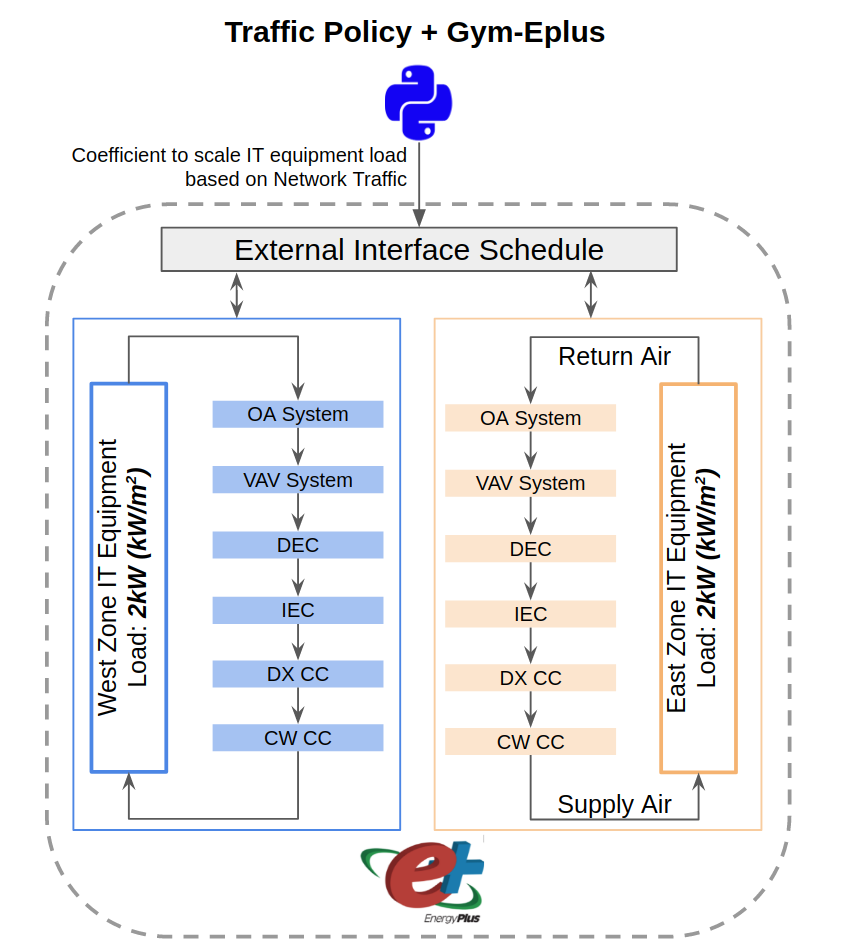
\includegraphics[scale=.25]{building_energy_model/TowardsEstimatingtheEcologicalCostsofInternetServices/paper_latex/img/python_eplus.png}
\caption[EnergyPlus and Traffic Model.]{EnergyPlus and Traffic Model.}
\label{img_ep_py}
\end{figure}

\begin{figure}
\centering
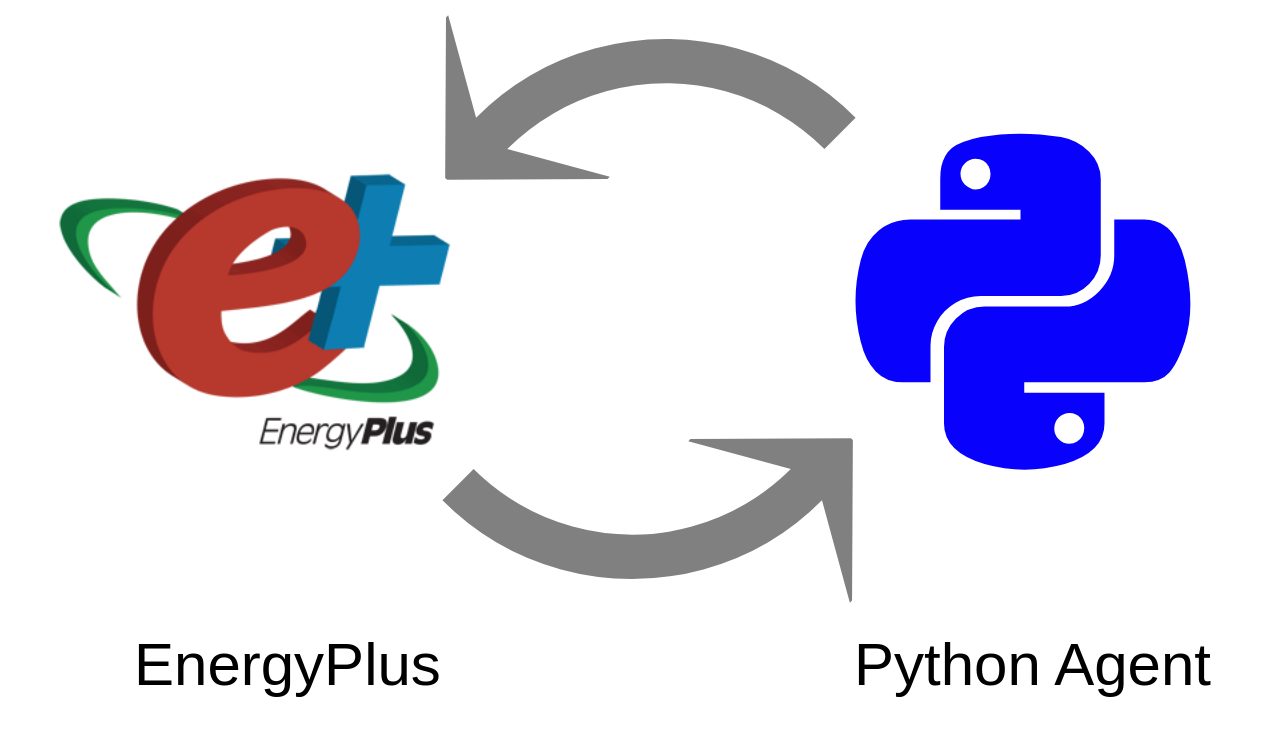
\includegraphics[scale=.10]{traffic_profile/images/agent_bem.png}
\caption{Dynamic Process Flow between EnergyPlus and the Python Agent.}
\label{fig:dyna-bem}
\end{figure} 

The simulator \deleted{allows}\added{integrates} algorithms that are aware of network traffic profiles programmed in Python \deleted{to interact} with EnergyPlus through the Building Controls Virtual Test Bed (BCVTB) \citep{wetter16}. The BCVTB interface from Gym-EPlus \citep{zhang19} is used to implement the interaction. \deleted{Python is chosen for the interface function due to its flexibility and the the granular level of program control and EnergyPlus is chosen due to it's established efficacy with building modeling. EnergyPlus is the US Department of Energy's state-of-the-art building modeling software. It features an extensible physics-based building thermodynamic and psychrometric modeling engine to simulate sub-hourly energy demands and occupant comfort values.} \added{This work extends Gym-Eplus capability by making it reset the IT load in DCs in addition to its thermal reset features. DCs have been explicitly supported in EnergyPlus since Version 8.3.0. Using the already supported DC variable for CPU load schedules in EnergyPlus, the xml file configuration as shown in Figure~\ref{cfg_xml} couples the Python module with EnergyPlus.}

\begin{figure} [!h]
 \lstset{
    language=xml,
    tabsize=3,
    %frame=lines,
    % caption=Test,
    label=cfg_xml,
    frame=single,
    rulesepcolor=\color{gray},
    xleftmargin=20pt,
    framexleftmargin=15pt,
    keywordstyle=\color{blue}\bf,
    commentstyle=\color{OliveGreen},
    stringstyle=\color{red},
    numbers=left,
    numberstyle=\tiny,
    numbersep=5pt,
    breaklines=true,
    showstringspaces=false,
    basicstyle=\tiny,
    emph={food,name,price},emphstyle={\color{magenta}}}
    \lstinputlisting{building_energy_model/code_cfg.xml}
\caption[EnergyPlus Variables reset by Python.]{EnergyPlus variables.cfg used to integrate Python and EnergyPlus. Other variable maps from GymEplus are listed in the variable.cfg, but not used in these simulations.}
\label{cfg_xml}
\end{figure}


\added{The baseline EnergyPlus model of the data center is adapted from Moriyama \citep{moriyama18}. Moriyama's building shell consists of two data center rooms. The first room, the West Zone is 232 square meters and the second room, East Zone, is 259 square meters. Each data center room has dedicated mechanical and electrical equipment that are symmetrical to each other. Throughout the simulations the building envelope, mechanical, and electrical modeling objects are not modified from the baseline. However, for this research, as the goal is to represent hyper-scale DCs; the IT equipment objects are changed to closer resemble the current practices in this class of DCs based on one of the authors industrial experience.}

% To closer resemble the current practices, the EnergyPlus IT object is defined based on one of the author's experience leading DC projects for severel large search engines and social media companies.   

\added{Three statically configured changes are made to the baseline model's ITE object. Namely the changes are; server inlet temperature, fan power ratio compared relative to the overall server power, and the CPU power density fields are changed. The typical EnergyPlus ITE object for each zone is provided in Figure~\ref{ite_object}. First on line 16, the server entering air temperature is changed to $25^{\circ}C$ from $15^{\circ}C$. Second, on line 12 the fan power fraction is changed to 0.10 from 0.40. The last static variable change increases the load density of the data center to 2 $\frac{kW/m^2}$ from 0.2 $\frac{kW/m^2}$ on line 8. Details on how this power density was derived is provided later in Algorithm~\ref{rack_power_counts}}.


\begin{figure} [!h]
 \lstset{
    language=fortran,
    tabsize=3,
    %frame=lines,
    % caption=Test,
    label=cpu_load_schedule_reset,
    frame=single,
    rulesepcolor=\color{gray},
    xleftmargin=20pt,
    framexleftmargin=15pt,
    keywordstyle=\color{blue}\bf,
    commentstyle=\color{OliveGreen},
    stringstyle=\color{red},
    numbers=left,
    numberstyle=\tiny,
    numbersep=5pt,
    breaklines=true,
    showstringspaces=false,
    basicstyle=\tiny,
    emph={food,name,price},emphstyle={\color{magenta}}}
    \lstinputlisting{building_energy_model/code_ITE.idf}
\caption[EnergyPlus IDF ITE Object]{EnergyPlus ITE Object Defintion. New features of EnergyPlus 8.9 are denoted with *.}
\label{ite_object}
\end{figure}

\added{The only dynamic variable change to the ITE object definition specifies the dynamic CPU Loading Schedule\_RL on line 10 of Figure~\ref{ite_object}. This new schedule replaces the original schedule, CPU Loading Schedule. Both of these schedules are shown in the IDF snippet in Figure~\ref{cpu_load_reset}. The CPU Loading Schedule\_RL is called from the IDF as an external interface through the BCVTB. For the BCVTB and EnergyPlus interface, this new schedule is mapped between the two software platforms in the variable.cfg file on line 38. Then at each time-step, a value for the CPU load is passed from Python to EnergyPlus. The passed value is multiplied by the CPU power density from line 8 of Figure~\ref{ite_object} for the simulation time-step.} 

\begin{figure} [!h]
 \lstset{
    language=fortran,
    tabsize=3,
    %frame=lines,
    % caption=Test,
    label=cpu_load_schedule_reset,
    frame=single,
    rulesepcolor=\color{gray},
    xleftmargin=20pt,
    framexleftmargin=15pt,
    keywordstyle=\color{blue}\bf,
    commentstyle=\color{OliveGreen},
    stringstyle=\color{red},
    numbers=left,
    numberstyle=\tiny,
    numbersep=5pt,
    breaklines=true,
    showstringspaces=false,
    basicstyle=\tiny,
    emph={food,name,price},emphstyle={\color{magenta}}}
\lstinputlisting{building_energy_model/code_cpu_load_schedule.idf}
    
% \lstinputlisting[language=fortran]{code_cpu_load_schedule.idf}
\caption[EnergyPlus IDF load Reset]{EnergyPlus IT load reset schedule definitions. The Schedule: Compact is replaced with the schedule defined in the External Interface: Schedule.}
\label{cpu_load_reset}
\end{figure}

\added{There are two ways to input the IT power load into EnergyPlus. The first is the unit count and unit-power method. The second is the power-density method. As seen above the floor area density method is used for this work. The density method is more conducive to scaling with the building size than the unit-power method. Algorithm~\ref{rack_power_counts} indicates the steps used to translate the properties from a actual hyper-scale data center to Moriyama's model. The density ($\rho$) is simply the product of the total provisions power for the IT equipment on the server floor ($P_f$) and the total server floor area ($A_F$).}

\added{Although expressing the IT density as a constant value over the entire floor area suffices for EnergyPlus' view of the IT load as a lumped thermal parameter, it is a naive representation of the power distribution on the floor. In realty racks are not placed evenly across the entire server floor, but are placed in rectilinear arrangements, as represented by $A_r$ in Algorithm~\ref{rack_power_counts} and illustrated in \ref{img_server_room}. By following the equations in Algorithm~\ref{eq:area_for_racks}, the rack counts and rack unit densities can be obtained and the method of entry can be changed.}

\begin{figure} [!h]
\centering
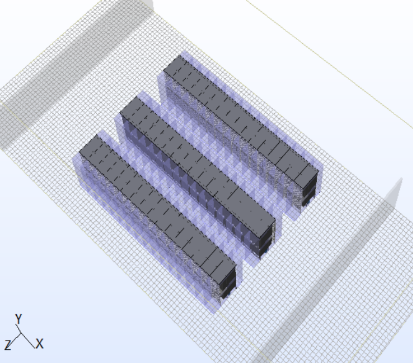
\includegraphics[scale=.5]{methodology/images/server_room.png}

\caption[Server room layout]{Server room layout. The gray elements in the figure are the hot aisles and the light purple elements are the server racks. The objective of the cited work was to determine the optimal spacing of adjacent racks across hot-aisles.  Image from \cite{sahini16}}
\label{img_server_room}
\end{figure}
  \begin{algorithm}
    \caption{Rack Counts from Building and Power Properties}
    \begin{algorithmic}

      \STATE $\rho= \frac{P_{f}}{A_{F}}$

      \STATE $A_{r}= A_{f} \times F_{f}$
      \STATE $R_{\#}= \frac{A_{r}}{R_{a}}$
      \STATE $P_{rs} = \frac{P_f \times (1-F_{n})}{R_{\#}}$
      \STATE $P_{rn} = P_{rs} \times F_{n}$
      \STATE $P_r = P_{rs} + P_{rn}$
      
      \STATE{\bf{Where}}: \\
        \hspace{.2in}$\rho$ = Power Density of server floor. This value is used in the EnergyPlus Models. \\
        \hspace{.2in}$A_{f}$ = Total floor area.  \\
        \hspace{.2in}$A_{r}$ = Area available for rack deployment.  \\
        \hspace{.2in}$R_{a}$ = Rack footprint area. \\
        \hspace{.2in}$R_{\#}$ = Rack count.\\
        \hspace{.2in}$P_{f}$ = Provisioned power for IT for server floor.\\
        \hspace{.2in}$P_{rs}$ = Power for rack server equipment. \\
        \hspace{.2in}$P_{rn}$ = Power for rack network equipment. \\
        \hspace{.2in}$P_{r}$ = Total power of rack. \\
        \hspace{.2in}$F_{f}$ = Fraction of $A_{f}$ that is deployable with Racks.\\
        \hspace{.2in}$F_{n}$ = Fraction of power to rack allocated to network devices.
        
        
        
    \end{algorithmic}
    \label{rack_power_counts}
  \end{algorithm}

\deleted{Without the Python feedback loop, EnergyPlus is a hermetic suite in which simulation run-parameters are defined in a configuration file; namely the IDF. In the default case, EnergyPlus modeling workflow serially runs the simulations \deleted{and then users get to review the results of each simulation at} \added{to} completion. Iterating on the parametric values requires \added{manual} editing of the IDF file and re-running of the entire simulation. This proposed simulation specifically defines a loop in Python which iterates over a list of load coefficients derived from the network traffic corresponding to the cooling load for each simulation time step.} 

\added{Now, the CPU Loading Schedule\_RL as passed in from the Python program to EnergyPlus is described. The basis for the schedule is a network traffic model built upon simulations of real world network traffic for a global service. The choice to characterise the DC IT equipment load with bandwidth of network traffic is superior to the usual hour-day-week schedules as an operational model because (1) most DCs serve international users across many time zones. (2) the DC workloads are known to not be stable across time. (3) network traffic is conducive to predicative models based around world events and seasons.} 

\deleted{The traffic profile of an internet service is an intrinsic property of the service.} Characterizing the traffic profile for an online service platform requires granular data that spans across a wide temporal range. However, due to the proprietary nature of the internet industry such data that allows for building level traffic profiles is not publicly available. Therefore, in this research a network traffic simulator is created. The objective for the simulator was to represent a globally distributed online platform indicative of real world user demand. To represent a global service, the load factors in this article reflect visits to 145,063 Wikipedia pages over an 18-month period as provided by Kaggle \citep{kaggle17}. In this work, publicly available information about Wikipedia's infrastructure establishes the geographical locations for the DCs as illustrated in the map in Figure~\ref{fig:dc_map}.

\begin{figure}[!h].
\centering
\includegraphics[scale=0.45]{building_energy_model/img/dc_locations.png}
\caption[DC Locations]{Data Center Locations Map. SFO: San Francisco, CAR: Carrolton, TX, ASH: Ashburn VA, AMS: Haarlem, Netherlands, SIN: Singpore.}
\label{fig:dc_map}
\end{figure}

One issue with the Kaggle data set is that it just provides a time series of page visits agnostic of source location (ie user location) or serving DC. For evaluating DC level workloads, the pages were mapped to a DC \added{location} as part of a pre-processing step of this research. The pre-processing required \added{handling} raw URL strings and parsing out it's language hash markers. Then, countries where these languages are the official languages are mapped to the nearest Wikipedia DC to indicate the traffic to each DC. \added{The step-wise procedure is in indicated in Table~\ref{table: url2dc}.}

\begin{table}[!h]
\caption[Steps to convert Raw URL to DC Network Traffic]{Steps for converting URL to traffic} \label{table: url2dc}
\begin{small}
\begin{tabular}{c|l}
\hline \hline
Step 1:& Map language to page by parsing URL \\
&structure. \\
\hline
Step 2:& Map languages to countries where they \\
& are the first tongue. \\ 
\hline
Step 3:& Map ingress sites to countries with \\
& minimum distance function. \\
\hline
Step 4:& Get the distribution of the number of \\
& countries served by each ingress site. \\
\hline
Step 5:& For each ingress site; sum up the daily \\
& views of pages in all language. \\
\hline \hline
\end{tabular}
\end{small}
\end{table}

The procedure resulted in the seven languages being routed by a minimum distance function from any country that they are the official language to the nearest DC site. Treating each of the seven languages as a service \deleted{allows this research to have an abstraction of the (Moriyama , et al., 2018) service which is intuitive to reason about as indicated in Figure~\ref{fig:lang2dc}} \added{provides an abstraction that makes each language an isolated platform. 

Figure~\ref{fig:lang2dc} shows curves with all languages to a particular data center aggregated together. These curves are translated to a coefficient that scales the IT load indicated on line 8 of Figure~\ref{ite_object}. The coefficients for each data center are normalized to the maximum traffic volume; i.e. max traffic indicates the upper bound with a coefficient of 1. These coefficients are independent across the five data centers.}

\begin{figure}.
\centering
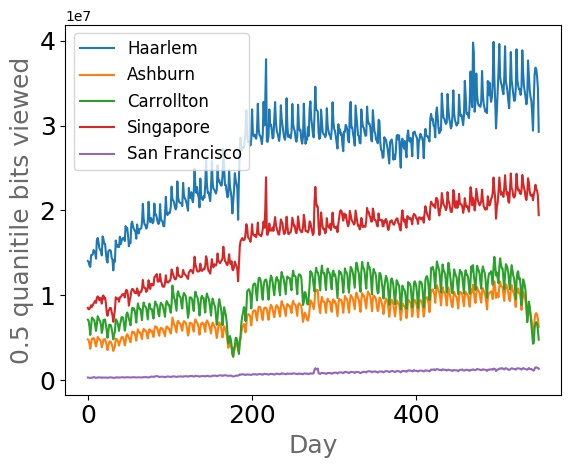
\includegraphics[scale=0.45]{building_energy_model/img/lang2dc_curve.jpg}
\caption[DC traffic with all languages summed]{Sum of English, French, German, Mandarin, Spanish, Russian, and Japanese traffic to each of the 5 DC locations.}
\label{fig:lang2dc}
\end{figure}

\deleted{To validate the impacts of resetting the proportional load factors, two specific simulations were run for each of the DCs from Figure~\ref{fig:lang2dc} The first is the novel dynamic load simulation and second configured as in \citep{moriyama18}. In both simulations nominal power density of the DC is set to 2kW/m2 and the auto-sizing feature is enabled for all HVAC equipment.} 


\deleted{\textit{Algorithm} \ref{Service Profile} indicates how the the service demand profile is generated. It is based on Kaggle's web-traffic data-set $(K)$ which is a time-series of the count of visits $(v)$ to 145,063 Wikipedia pages distributed across seven languages $(l)$ at daily intervals \citep{kaggle17}. In this work  pages $(p)$ are aggregated together by language and classified as a common service. $P_l$ is a list of all pages with the language $l$. The subscript $d$ represents individual DCs.  The demand for the service at a particular DC is obtained by the average quantile visits to the pages of the respective language as indicated by $P_{l}[d]$.} 

\deleted{\begin{algorithm}
\caption{Service Profile}
\begin{algorithmic}[1]
\REQUIRE{$K$} %Time series
	\FOR{$p$ in $K$} % Each Page in the time T
		 %For each lanugauge in T
		\STATE{$P_l = empty[$ $]$} % Create a unique table for each lanuage
		\STATE {$P_{l}[l] \gets p_l == l$  } % Populate matching langauge intot he luange table
		\FOR{$d$ in $range(K_d)$}
			\STATE {$P_{l}[d][quantile(v)] \gets \sum{P_{l}[l][d]}$} %Sum the visits, v per day to get service profile
	\ENDFOR
	\ENDFOR
\end{algorithmic}
\label{Service Profile}
\end{algorithm}}

\deleted{Figure~\ref{fig:lang2dc} illustrates the service profile for the data range and notes the seven languages. The y-axis is the number of page views on a $1e^8$ scale, the x-axis spans the date range, and the curves represent each of the seven languages.}
Next we discuss the results from a model build with the methods discussed in this section.

% -------------------------------------------------------------------------------------------------------------------------------
\section{Results}
% -------------------------------------------------------------------------------------------------------------------------------

\added{The traffic aware EnergyPlus models are simulated for each data center location through GymEplus in a batch process loop. In the batch workflow, the same IDF file is used to represent all of the data centers shown on the map in Figure~\ref{fig:dc_map}; except their local weather files are changed by the scripted loop. In} these reset load (RL) simulations, \added{at each time step} the traffic load factor is pulled in \deleted{by}\added{from} the Python program and is passed to EnergyPlus \added{by BCTVB. This demonstrates that using an external interface (such as logic scripted in Python), building energy models can facilitate the analysis of a network of data centers in a single workflow. 

A second set of simulations without the external interface (NoRL) were also run for each DC with a similar workflow to quantify the energy use with default CPU loading schedule shown in Figure~\ref{cpu_load_reset}.} The total annualized energy use of the two models is plotted for comparison in Figure~\ref{fig:total_energy_comp}. The purple bars indicate the simulations in which the CPU loads are reset at each time-step (RL), and the green bars indicate simulations without interactive resetting of the loads (NoRL). For Singapore (sin), San Francisco (sfo), and Ashburn (ash) the RL simulations result in higher annualized energy compared to the NoRL model. While for Amsterdam (ams) and Carrolton, TX (car), the RL model results in lower energy demand compared to the statically configured load from the NoRL simulation.

\begin{figure}.
  \centering
  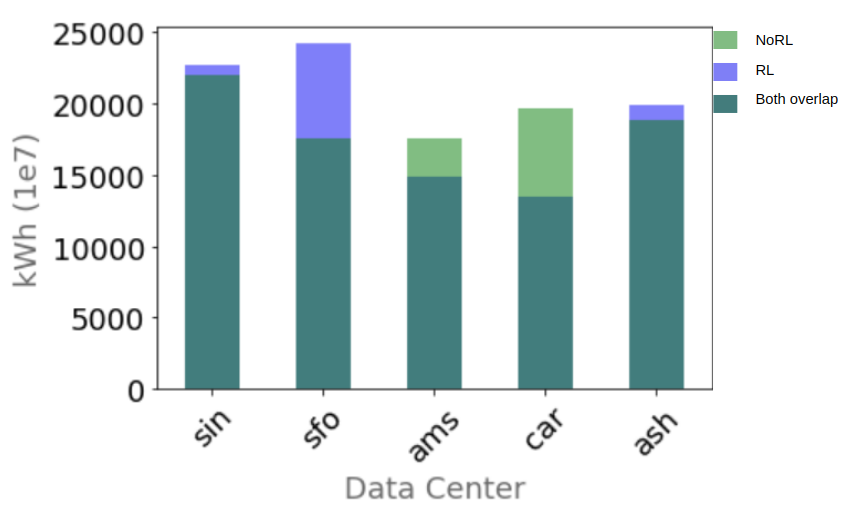
\includegraphics[scale=0.275]{building_energy_model/img/cpu_comps_3legend.png}
  \caption[Comparison of energy demand for two models]{Total Site Energy Difference between statically configured IT load and dynamically reset IT loads.}
  \label{fig:total_energy_comp}
  \end{figure}

The variations in the relative energy demands between the two models can be attributed to the CPU load profiles as illustrated in Figure~\ref{fig:cpu_comps}. The figure illustrates the time series plot of each DC analyzed through the RL simulations with line curves. The x-axis indicates the hour of the year and the y-axis indicates the CPU load for each respective DC. \deleted{Examining}\added{The CPU profiles for each DC that} their \deleted{values appear quite}\added{average values} are distinct from one another. Carrolton and Ashburn appear to have  \deleted{strong}\added{noticeable} seasonal patterns. Amsterdam and Singapore DCs show irregular oscillations in demand throughout the year\added{, but have a tight band}. The San Francisco DC has a constant line. This constant demand is due to the load not varying much from the peak capacity in the traffic profile that was used for the site. 

In contrast to the distinct CPU load profiles of the RL loads as discussed above, with default schedule configuration of IT load profiles used in the NoRL models, the CPU loads at all the DCs are identical to each other. The static property of the NoRL model is also indicated in Figure~\ref{fig:cpu_comps} by the gray band. The gray band is actually composed of line curves that cycle diurnally with the given schedule.


\begin{figure}
  \centering
  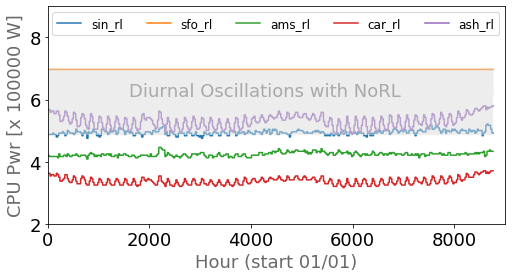
\includegraphics[scale=0.45]{building_energy_model/img/cpu_comps.png}
  \caption[CPU Time Series]{Time series of the total CPU power at each DC (see legend). Gray area indicates the daily demand cycle that the IT equipment creates with NoRL.}
  \label{fig:cpu_comps}
  \end{figure}

\deleted{Given this understanding of the cyclic loads, the relative variance between the RL and NoRL simulation’s total energy results can be reasoned about by considering the profile of San Francisco DC as an extreme example. San Francisco’s RL model does not vary the CPU load, whereas the NoRL model does. With the constant peak load, the San Francisco DC’s RL simulation indicates higher utilization than the NoRL model therefore demanding more power.}

\added{Figure~\ref{fig:stacked_pue} shows a stacked histogram for the set of DCs modeled. This plot shows that even with a identical building systems the efficiency of each DC will vary across the globe. One major contributor to this difference is obviously the local weather conditions which DC operators can;t control. However, the second contributor is the workloads at the DC. The workload is a variable that can be controlled by the DC operators.}

\begin{figure}[!h]
  \centering
  \includegraphics[scale=0.4]{building_energy_model/img/pue.jpg}
  \caption[Stacked PUE Histogram]{Stacked PUE Histogram for all five data centers .}
  \label{fig:stacked_pue}
  \end{figure}

In the next section, the extensibility of the traffic based building energy model towards predicative scenarios and the potential to use this framework to exploit 'free capacity' are discussed.  


%-------------------------------------------------------------------------------------------------------------------------------
\section{Discussion}
% -------------------------------------------------------------------------------------------------------------------------------
\deleted{To reason about the EnergyPlus RL results from Figure~\ref{fig:total_energy_comp} for total energy, the San Francisco site again serves as an example. In the figure, the total site energy used for the annual model is $1.19 \times 10^7$kWh. Through the course of 8,760 hours the power demand for the DC is 1,359 kWh on average; translating to an annualized PUE value of approximately 1.36 due to the base IT load density of $2 kW/m^2$ (with a network load coefficient set to 1 for all hours). The PUE values of the other sites are more complex to reason about without further processing of the data, as they all operate at part load conditions.}

One obstacle for building operators for using building energy models to make operational decisions is that working with these models requires deep knowledge about the software implementation of the models. The one variable that operators control are the IT loads and allowing the IT loads to characterized by external software in building energy models can allow operators to do some interesting things. For example, operations teams can simulate perceived future changes to their work loads. As mentioned above predicative modeling is feasible when using network traffic as the proxy for IT loads. Network traffic has been shown to be predictable within reasonable accuracy for internet services by Linkedin \citepp{zhuang15}. Figure~\ref{fig:arima_bem} shows the predicative models for four of the data center studied in the simulations for this work. 


\begin{figure}[!h]
  \centering
  \includegraphics[scale=0.25]{img/_arima.png}
  \caption[ARIMA for BEM]{Forecasting Model of the Traffic.}
  \label{fig:arima_bem}
  \end{figure}

In this research the network traffic serves as a proxy for CPU utilization. In practice the network traffic and CPU have complex correlations that can't be generalized with the presented approach. In production DC environments representative correlations can be obtained between network traffic, the IT workloads the the traffic instantiate, and the workload's CPU demand. However, proving such correlations is out of scope of research. \added{Nonetheless, every data center will be subject to its own traffic models due to it being an intrinsic property of the service.}

This research assumes that all the facilities are of the same size in terms of power, space, and cooling. From looking at Figure~\ref{fig:lang2dc}, San Francisco site has a much lower traffic profile than Haarlem. The claim that the same power capacity handles this range of traffic requires another assumption. This assumption is that the CPU-Network ratio vary from site to site. For example a bit of network traffic generates 40 times as much CPU workload in San Francisco as it does in Haarlem. This assumption is the basis for normalizing the traffic coefficient, as described by the discussions on Figure~\ref{fig:lang2dc}. This is a realistic condition in DC fleets were have different generations of IT hardware in operations at various DCs. Or this condition can be encountered when software optimizations to specific workloads are done for targeted consumer markets that are geographically segregated. Nonetheless, since the network coefficient is bound between 0 and 1, and network-workload-CPU model can be supported in the same framework. 

\added{As an example of free capacity mentioned above, consider a design day dry-bulb temperature of 105$^{\circ}$F. When a peak in IT workload occurs on a more favorable day, say 95$^{\circ}$F, the computer room air conditioner heat rejection equipment needs 50\% of the designed power value \citep{liebert20}. With a slight modification in the electrical infrastructure, this difference can opportunistically be allocated to IT workloads. However, slight the the electrical modification, the decision is most cost effectively made during the design phase of the the facility. This influence on the design presents a case for using the fine grained load aware model presented incpu\_load\_reset the work during the design phase as-well.

Opportunistically using 50\% of the provisioned power from the cooling equipment to power the IT equipment requires some further insights about DC operation. First, the 50\% claim is based on nameplate full load amps (FLA) for two different dry-coolers (Models D-466 & D-880) are matched with a 105kW indoor computer room air conditioner (DC Model 105). One of the dry-coolers is rated at 95$^{\circ}$F and the other is rated at 105$^{\circ}$F \citep{liebert20}. The FLA for these units are 14 Amps and 28 Amps respectively. Physically this translates to breaker sizes, wires sizes, utility power feed reservations, and back-up generator reservations decisions being made using this value. Second, with the claim it is assumed that the power draw has the same proportional scaling with loads cross both sets of units. 

To summarize the last two paragraphs more explicitly, in conditions where the ambient enthalpy is lower then the design day, \deleted{the additional capacity of the cooling equipment are}\added{electrical provisions beyond the real-time demand relative to the design values are} stranded. \added{This is an important consideration for a building class where its utility is measured by the power delivered to IT equipment use. Anytime when the stranded power can be re-purposed from auxiliary infrastructure (such as chillers, cooling towers, and transformers) to the IT equipment, it leads to compelling return on investment cases.}

% This is a naive assumption and such a practice is not suitable for the design phase building energy models where equipment must be sized for worst case conditions. However, the claim suffices to demonstrate that on non design days there is stranded power in terms of the physical capabilities of the electrical infrastructure. For a building class where its utility is measured by IT power density; any opportunistic usage of power is highly valuable. As a concrete example, when the part load of the dry cooler is known for future states in time, major capacity constraints in DC such as the utility power reservations and back up generator reservations can be relaxed during that time range. This would allow the IT to be oversubscribed relative to its design conditions, yet the building would still be within its overall power envelope. 

%\added{utility power reservations and back-up power generator reservations. More explicitly, during the part load operations of the cooling plant when their electrical demand is lower then their design values; the headroom in power infrastructure from the cooling equipment can be safely supplied to IT equipment. The rerouting of the available power increases the supportable IT load and essentially yields 'free capacity' beyond the design values of the IT load}% 
}

% \added{The design power input represents the electrical power loading of servers. In practice the CPU is a dominate energy consumer of IT equipment but it’s not the only power consumer. Aside from the fan and power supply unit which are explicitly defined in the ITE IDF object, it is unclear how the power demand for hard disks, random access memory, and other parts are accounted for in EnergyPlus.}

% Another benefit for externally configuring traffic changes to the data centers is that when new data centers are built, the traffic routing changes. Having an external signal for the traffic allows operators to run the models to check operations without having to change the building systems.

%Independently normalizing each data center to max workload is sensible as each data center may have different hardware with various performance behaviors. For example it may take more resource at one site to complete a user request as it does at another site.
% -------------------------------------------------------------------------------------------------------------------------------
\section{Conclusion}
% -------------------------------------------------------------------------------------------------------------------------------
There are two notable benefits of resetting the IT load values outside of the IDF file. First, defining load values for each hour in the IDF file is toilsome and error prone. The toil of entering values for each simulation time-step would require 8,760 entries in the file. This increases the chance of introducing errors into the simulation. Second, the external definition allows more sophisticated logic to control the time-step variables. In this article, only the IT load factors were reset, none-the-less the same interface can reset many other simulation run-parameters with similar logic. An example of a feedback logic is reinforcement learning, which can be framed to globally optimize the systems and is an topic for future research. 

The traffic profile used in this article are representative of a globally distributed service’s user facing workloads and suffices for purposes of demonstrating the dynamics of DC operational loads. Each real-world service will have a unique profile resulting from a combination of critical and opportunistic back-end workloads. The modular construction of this model is conducive for incorporating the other workloads and being inclusive of back-end workloads.

Figure~\ref{fig:lang2dc} aggregates all the languages to provide an overall building simulation. However future work that need to assess a service platform can create multiple ITE objects in EnergyPlus and quantify the energy demands for each in isolation.
%---------------------------------------------------------------------------------------
\section{Abstract}	% Section headings need to be upper and lower case.
%---------------------------------------------------------------------------------------
\addtocounter{section}{1}


% Globally distributed internet services are ubiquitous today. These services are driving the demand to build mega-watt scale data center facilities (DC) distributed through out the globe. 

Over the last decade, operational efficiency optimizations in data center (DC) facilities designs have curtailed their absolute power demands. However, their physical footprint is still growing. This growth in capacity may offset the efficiency gains at best or it may even dwarf the them in absolute terms. Offsetting effects such as the these make system level life cycle environmental footprint evaluations complex for distributed services operating in these DCs. 

To support system level evaluations for services operating in DCs, this research uses simulated network traffic profiles and coincident energy generation source aware building energy models (BEM) to evaluate the marginal carbon footprint of a globally spanning network of data centers. The result of this research is a BEM based framework that can be used in environmental decisions to characterize DC life-cycle costs.




%---------------------------------------------------------------------------------------
\section{Introduction}
%---------------------------------------------------------------------------------------
Globally distributed internet services are ubiquitous today. These services are driving the demand to build mega-watt scale data center facilities (DC) distributed through out the globe. In a 2015 study data centers were forecast to consume as much as 13\% of the global energy production by 2030 \citep{andrae15}. More optimistic models form the US Department of Energy for the US showed a curtailment with up to fifty percent decline in energy compared to the industry's use of 2\% of the power produced by the national grid in 2005 as a result of using state of the art efficiency and consolidation practices \citep{Shehabi16}. As more and more parts of society are transitioning to data center dependent online paradigms, the absolute demand of data centers is growing. The volume of growth is exemplified by the capital costs being invested across the world in constructing these data centers.

The growth in data center capital construction costs will reach \$89 billion by 2027, a significant increase from the \$45 billion spent in 2018 \citep{dcmarket19}. Capital costs aren’t the only commitments for data center owners however. DC owner\textsc{\char13}s also incur significant operational costs throughout the entire operational lives of their facilities.  

Over a 20-year life of a continuously operating data-center facility, the use-phase energy costs can exceed its capital costs while having a much larger ecological footprint. Given the accumulation of costs and impacts over the life of data centers, there is a need for a robust model the couples the information technology (IT) and building systems with their energy supply sources through its useful life. In this article a geographically extensible model that accounts for the workloads, building systems, and power utility grid is presented.

In the rest of this paper a model for coincident energy demand and marginal energy costs (MEC) of a set of data centers is proposed and developed. First, the proposed method uses a hybrid model consisting of EnergyPlus and Python programming modules as developed by the researcher in \citep{kumar20}. For this article, the researcher's original hybrid model is modified as described in the methodology section to be more indicative of the current operations of cloud data centers. Then second, the resulting time series of operational energy demand profile is used as input to a Python based open source MEC simulation tool that is also extended as described in the methodology section. The baseline MEC model is described next. 

The MEC calculations are based on the Dispatch Optimized Systems Cost of Energy (DOSCOE) model developed by Platt \citep{platt17}. DOSCOE provides a linear programming platform that computes the monetary costs and several environmental emissions associated with operating a mix of dispatch-able and non-dispatch-able energy sources. In this context, dispatch-able energy sources are those that can be controlled to meet demand. Natural gas power plants are examples of dispatch-able source of energy, where the plant operators can control the mass flow rates of the combustion gases to curtail generation rates. On the contrary are the non-dispatchable sources, where the energy generation is dependent on extrinsic factors. An example of non-dispatchable energy source is solar; where cloud cover greatly effects the generation rate and no power can be generated at night.

Modeling the costs for a mixture of dispatchable and non-dispatchable generators is complex as most non-dispatchable sources are only accounted for as opportunistic supply sources when sizing the power generation infrastructure. By dsign the dispatchable generators are sized to meet the full demand in a worst-case condition when no dispatchable power is available \citep{platt17}. However, when non-dispatchable power is opportunistically available, it supplements the grid; allowing dispatchable sources to be turned down to part loads. This saves fuel costs for dispatchable sources (ie natural gas generators), but it leaves their physical infrastructure stranded and underutilized. This research’s coupling of the DOSCOE model with a BEM quantifies the monetary and ecological costs associated with operating data centers in grids with optimal mixtures of energy sources bound by physical constraints to be evaluated by matching the marginal costs of energy with data center demands on hourly intervals. Furthermore, the resulting model is inclusive of the stranded costs of the underutilized power infrastructure.

In the next section, Background, informative context is provided to set the proper use-case for this framework. Then in the Similar Works section, past literature which have quantified the ecological life cycle cost of data centers and internet services are summarized. In the Methodology section, the two main modules of the software implementation of this research are presented. Specifically these modules are a modified version of hybrid building energy model and a novel MEC model based on DOSCOE. After the details of the models are presented, the results are discussed in the Results and Discussion section followed by the Conclusions.


%---------------------------------------------------------------------------------------
\section{Background}
%---------------------------------------------------------------------------------------
Data centers are critical to modern internet experiences for billions of people. They are the key enablers for disseminating information in real time regardless of people's location. As an example of location agnostic services geographical dispersed infrastructure, Figure~\ref{fig:net_diag} illustrates a geographically distributed architecture that enables data centers to provide globally consistent internet experience that have become the status quo over the last decade. Distributed software architectures implemented in the server clusters at the leaf-nodes consist of a collection of autonomous computing resources that appear to its users as a single coherent system \citep{tanenbaum}.

In Figure~\ref{fig:net_diag}, a data center network stack with three hierarchical WAN layers are shown. The first hierarchical layer, the global level, has a wide area network (WAN) connected to two internet service providers (ISP) as its root node. For the purposes of this work the WAN is an abstraction of a network that connects a set of data center facilities with each other. The second layer of the global level are the metropolitan regions. In this layer, the ISP links are shown as coming in from top and the outgoing links from the bottom serve local distribution networks to buildings within the metropolitan areas. The final layer of the global level are the data center buildings, where the global network links connect to clusters of servers. Inside each data center there may be another independent hierarchy as shown by the server clusters. The physical network links shown in Figure~\ref{fig:net_diag} connect the buildings to each other through the WAN. However, the physical links (Pink, Magenta) is transparent for the clusters, which directly communicate with each other through logical links (Gray, Green, Red).

\begin{figure}
  \centering
  \includegraphics[scale=.2]{marginal_energy_cost/img/net_diag.png}
  \caption[Generic Network Topology]{General Topology of data center networks. The 1:1 metropolitan area to building relationships are shown for clarity only. Pink: indicates the first layer - ISP-Metropolitan links (physical). Magenta: indicates the second layer Metropolitan-DC Building with a full mesh connection (physical). Gray: represents the cross-connection between Data Centers (logical). Green/Red: Cluster to Cluster links (logical).}
  \label{fig:net_diag}
  \end{figure}


Large cloud data center operators have championed WAN systems for global up-time (service availability) and user experience optimizations \citep{sushant13} \citep{hong13}. Cloud data centers are a specific class of data centers. They serve business functions that require custom IT and building systems tuned for optimality in total costs of ownership models. These facilities house numerous services that can be controlled by network load balancers, with each data center limited by its physical infrastructure's capacity. As described in Sushant and Hong, the WAN networks can shift loads between data center on command.  The efficacy of a strategy for shifting computational loads depends on the capacity headroom of the physical resources at the data center where the loads are shifted to. 

The fungibility of locations enabled by WANs is desirable from an service application performance point of view as latency can be significantly reduced for specific markets and applications by minimizing the round trip communication times with consumers. Given the popularity of the public clouds, the use of network aware energy models for data centers extends beyond just data center construction and plant operations. Extending beyond the physical data center, network aware energy models can be used by internet services that operate public clouds where a given service is sharing the resources with may other independent services.    

In the context of BEMs, WAN's make the IT workloads temporally (and geographically) unstable, rendering it elusively for building modelers to reason about. As an example of temporal and geographical instability of data centers, Figure~\ref{fig:google_activity_dist} \citep{barroso18} shows the difference in utilization rates for two server clusters from Barroso's operational experience. This behavior of IT loads is something that WAN aware BEMs can help characterize and exploit. One possible means of exploitation is to flatten the peak of each cluster by routing the excessive workloads to another similarly provisioned cluster with lower coincident demands and sufficient building systems capacity headroom. However, building energy simulation need to be aware of more then just energy to make the right environmental decisions. To effectively optimize environmental objectives, BEMs coupled with MEC models can quantify the energy's global warming potential in terms of carbon footprint to shift loads from one building to another.

  \begin{figure}
    \centering
    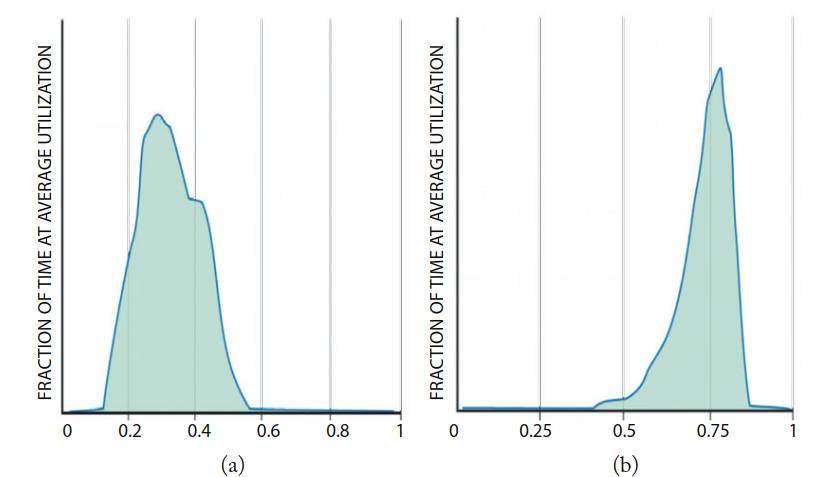
\includegraphics[scale=.2]{marginal_energy_cost/img/google_activity_dist.png}
    \caption[Usage profiles of two production DC Clusters]{Activity distribution of a sample of 2 clusters, each containing over 20,000 servers, over a period of 3 months. The x-axis indicates the server utilization rates (0 to 1) and the y-axis indicates the fraction of time during the 3 months \citep{barroso18}. The figure on the right (b) shows that peak utilization exceeds 75\% with little variances over the 3 months, whereas the right figure (a) shows that utilization is below 60\% at all times.}
    \label{fig:google_activity_dist}
    \end{figure}

Based on the literature reviews and references cited, there are no publicly available simulation frameworks that couple the dynamic data center workloads and the coincident carbon footprint associated with powering their load. The marginal cost of energy coupled building energy model described in this research is the first publicly available tool to allow owners, designers, and researchers to quantify the carbon footprint of data center operations accounting for granular supply and demand matching of power. Next, a literature review of past works concerning the carbon footprint of data-centers and digital services is presented in the Similar Works section.


%---------------------------------------------------------------------------------------
\section{Similar Works}
%---------------------------------------------------------------------------------------
There are two notable past works that look at the energy footprint for distributed sets of data centers. First, Tripadi considers hardware capital costs alongside with energy acquisition costs to quantify the total costs of ownership in \citep{tripadi17}. Tripadi\textsc{\char13}s framework is dynamic in terms of workloads but it is not aware of the building energy dynamics. In the second work, Kiani and Ansari describe a geographical load balancing strategy that exploits green energy mix in the utility grid \citep{kiani17}. However, their load balancing scheme doesn\textsc{\char13}t provide insights into how the load balancer evaluates the building energy demands or how the greenness of the energy supply is obtained. 

Using a life cycle assessment framework, Whitehead demonstrates a comprehensive data center site level life cycle costs analysis in \citep{whitehead15}. All energy use in Whitehead’s models were deduced from annualized PUE values, precluding coincident energy source evaluations with their framework. Similarly the Green Grid’s data center life cycle assessment guideline is limited to PUE as their suggested basis for the operational energy proxy \citep{tgg12}. The PUE metric is shown in Equation~\ref{eq:pue}, it has proven to be the most popular method for data center operational efficiencies since 2006 \citep{wiki_pue}.

    \begin{equation} \label{eq:pue}
    PUE=\frac{E_{total}}{E_{IT}} 
    \end{equation}
    \begin{center}
    $E_{total}$ = Total Power Used at Facility
    
    $E_{IT}$ = Power Consumed by IT Equipment
    \end{center}
    \vspace{.2cm}
    

Other’s have evaluated the costs of internet services \citep{koomey08} \citep{shehabi14}. Taylor and Koomey quantify the energy and greenhouse gas implications of online Advertising circa 2008. While Shehabi evaluates the energy and greenhouse gas implications of video stream circa 2014 \citep{shehabi14}. Together these works provide a taxonomy that can be followed to assess internet service costs in terms of energy use. 

%---------------------------------------------------------------------------------------
\section{Methodology}
%---------------------------------------------------------------------------------------
In this section the MEC model\textsc{\char13}s coupling with the BEM is described. The resulting model maintains a strict partition between the two technical domains. The first part of the model simulates the hourly energy demands of a set of five data centers in EnergyPlus (EP) using the method demonstrated in \citep{kumar20}. These data centers are distributed across the globe as shown in Figure~\ref{fig:dc_locations}. Then in the second part, the data center demands are matched with the respective region\textsc{\char13}s utility power generation sources for the coincident hour to assess the MEC during that hour. These parts are described in the following subsections. 

\begin{figure}
  \centering
  \includegraphics[scale=.40]{marginal_energy_cost/img/dc_locations.png}
  \caption{Data center locations}
  \label{fig:dc_locations}
  \end{figure}

A fundamental component of the demonstrated implementation of this framework is the network traffic simulator from \citep{kumar20}. The simulation produces a time-series profile of the network traffic that a hypothetical service will get at a particular data center site. The hypothetical services are based on Wikipedia and segregated according to the natural language of the Wikipedia pages. By segregating services by natural languages allows the treatment of each language as a 'service platform'. With these network simulations, one or more languages can be supported from a single data center with the constraint that the sum of the IT workloads does not exceed the capacity of the data center facility. 

%---------------------------------------------------------------------------------------
\subsection{Building Energy Model}
%---------------------------------------------------------------------------------------
For the first part, a sufficient building energy demand profile is simulated as in \citep{kumar20}.  The IT workload profile characterizing the power and cooling load is obtained by using simulating the 50th quantile of daily network traffic to each data center using Kumar’s method from \citep{kumar20b}.  However in lieu of using EP release 8.6, the simulation in this work uses EP release 8.9. The changes found EP 8.9 are listed in NREL’s GitHub \citep{nrel_git}. The programmatic changes from EPv8.9 resulted in three notable differences between original BEM and the model presented here.  The first change was motivated by original BEM's runtime errors when setting $2kW/m^2$ as the IT equipment load density. This persistently led to thermal runaway conditions for the Singapore and San Francisco sites in EP release 8.9. In order to keep the building envelope form-factor and the construction materials the same, this simulation’s IT power load density is changed to $1.0kW/m^2$.

The second change was made to exploit a new feature for modeling supply and return air compartmentalization in EP release 8.9. In these simulations, the data center model has air distribution flow control with approach temperatures specified. Flow control with approach temperature method calculates the temperature differences between the IT hardware boundaries and the air handling equipment.  This method is more representative of modern data-center operations and allows modeling ASHRAE 90.4 Standard’s requirement of hot-aisle / cold-aisle compartmentalization. The alternate method in EnergyPlus considers the entire data center room as a well-mixed environment, consistent with the modeling from \citep{kumar20}. While using the approach temperature method, the cooling set-point is changed to 27 degrees Celsius from 25 degrees used in \citep{kumar20}. This 2-degree adjustment corresponds with the approach temperature between the air handling equipment discharge and the inlets of the ITE; as there is no mixing of the supply air before it enters the ITE. 

As the third and final change, the load distribution values in the IDF were revised from the SequentialLoad setting to UniformPLR. In the former, equipment is activated in the order listed in the IDF. With this specification each piece of equipment ramps sequentially from its idle state to full capacity, before subsequent equipment is enabled. In the latter load distribution specification, all equipment are loaded in parallel to each other. Another available setting for load distribution, the Optimal specification, was also tried for this field, but it crashed the simulations.

To validate that the proposed building energy model configurations with the above changes produce reasonable results, each data-center is simulated with two models. In the first model, the economizer for the direct evaporative cooler (DEC) limits are increased while in the second model the default settings are maintained. The summary of the changes are indicated in Table~\ref{table:tab01}, while the comparison of total site energy between the two models for each set of the simulations is illustrated in Figure~\ref{fig:total_energy_comp}. 

In Figure~\ref{fig:total_energy_comp}, the pair simulations for a DC site is presented in the single bar. In the figure the magenta bar part of the bar indicates the total site energy of the model with economizer dry-bulb temperature limits increased (RL). The light green indicates the default values (NoRL). The dark green part indicates where the two simulations overlap. From the figure it is observed that the increased economizer and the IT workloads resets lead to more energy use than the default values for three of the five DCs. While it maybe possible to fine optimal economizer settings, for this article it's concluded that the new settings from suffice. 

  
  \begin{table}[ht]
  \begin{small}
    \vspace{-10 pt}
    \caption{Economizer settings for the two models}
    \label{table:tab01}
    \centering
    \begin{tabular}{| c | c | c |c| }
      \hline
      IDF Object & Variable & Default & Increased\\
      \hline  \hline
      DC-OA & Econ. Max db-C & 23 & 28 \\
      \hline
      DC DEC & Evap. Max db-C & 20 & 28 \\
      \hline
    \end{tabular}
    \vspace{-8 pt}   % Please use appropriate negative vspace to remove the space above/below the Table
    \end{small}
    \end{table}

  \begin{figure}
    \centering
    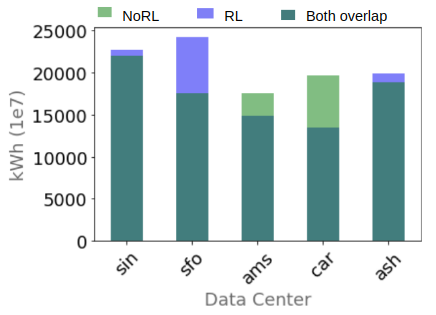
\includegraphics[scale=.50]{marginal_energy_cost/img/total_energy_comp2.png}
    \caption[Comparison of Economizer Settings in E+]{Comparison between increased economizer settings  vs. default IDF settings from \citep{kumar20} }
    \label{fig:total_energy_comp}
    \end{figure}

  The next subsection introduces the marginal costs of energy model, which will take the results from the BEM model described above.

%---------------------------------------------------------------------------------------
\subsection{Regional Marginal Costs of Energy}
%---------------------------------------------------------------------------------------
The second module requires a time-series profile of the electrical grid’s power source attributions, where the intervals of the power generation values match the BEM energy profile. The corresponding  site and regional grid model pairs are indicated in Table~\ref{table:tab02}. For this model the energy generation regional grid profiles are obtained from Platt, who provides profiles for 13 US regions in DOSCOE [5]. Singapore and Amsterdam data-centers grid profiles are constructed as described below.

\begin{table}[ht]
  \vspace{-10 pt}
  \caption{Data Center Site and Power Grid}
  \label{table:tab02}
  \centering
  \begin{tabular}{| c | c | c |  }
    \hline
    \bf{DC ID} & \bf{DC Location} & \bf{Regional Grid} \\
    \hline
    SFO & San Francisco, CA & California \\
    \hline
    CAR & Carrolton, Texas & ERCOT \\
    \hline
    ASH & Ashburn, VA & Midatlantic \\
    \hline
    AMS & Amsterdam & Netherlands \\
    \hline
    SIN & Singapore & Singapore \\
    \hline
  \end{tabular}
  \vspace{-10 pt}   % Please use appropriate negative vspace to remove the space above/below the Table
  \end{table}

  Each U.S region's grid profile is composed of hourly demands and corresponding production capacity of several power generation technologies. Hourly values for each region’s demand, solar, wind, coal, coal with cryogenic capture, coal amine gas scrubbing, and nuclear are defined. These grid regions are representative of three out of five of the data-center locations being simulated. 
  
  For Singapore, the International Energy Agency (IEA) provides a top down view of the annual energy production from various technologies. The IEA data shows that the renewable penetration in the energy supply for Singapore accounted for only 1.6\% of the total energy demand in 2016, the last year the data is available \citep{IEA17}. Due to this negligible contribution from renewable sources and lack of hourly generation data, it is assumed that all demand is met by natural gas power generators, consistent with other sources \citep{eia20}. The demand profile for Singapore in 2016 is obtained from \citep{sin16}.

  For the Amsterdam data center, energy profile of Netherlands is used. The IEA indicates that in 2018, 12\% of Netherlands's energy demands was met by renewable sources. This is a meaningful contribution from renewable, therefore a more granular generation profile is prudent as opposed to Singapore which did not require evaluations of the energy mix at any given time.  To formulate a more granular resolution of the Netherlands' generation, the IEA data is supplemented with data from the Open-Power-System-Data to characterize the time series profile of renewable energy \citep{ospd19}. OPSD provides hourly data for the renewable sources only. The balance of the energy demands in the Netherlands is met by fossil fuel-based generators, namely 35\% by coal and 42\% by natural gas \citep{eia20b}. The DOSCOE grid profiles don’t have any corresponding field for bio-mass, so the bio-mass generation indicated in OPSD is lumped in with the fossil fuel generators. In the discussion section, some validation for this approach is presented. The Netherlands also produces nuclear energy, but only the annual production rates were obtained \citep{eia20b}. In this works implementation of the DOSCOE, the annual nuclear production for Netherlands is distributed equally over the year and modeled as a constant (non-dispatchable) base load throughout the year.  

  The MEC coupled BEM algorithm is given below. In the algorithm two inputs are required. The first is DOSCOE[region], it is a two-dimensional array formatted as described in \citep{platt17}. It indicates hourly grid profiles of the power demand and power capacity of the available energy sources at the corresponding hour. The second input, traffic.language, is a one-dimensional vector indicating the network traffic to the respective site from \cite{kumar20b}. In the algorithm; for each language, it’s traffic to the respective data center is checked. If there are traces of a language routed to a site, the algorithm performs the BEM simulation by invoking EnergyPlus. This resulting demands from EnergyPlus are then added to the region’s grid demand profile. If a language does not have any traffic to a particular site than, the data center site does not do any work and the BEM simulation is bypassed.  

  \begin{algorithm}
    \begin{small}
    \caption{MEC coupled BEM algorithm}
    \begin{algorithmic}
      \REQUIRE DOSCOE[region] \& traffic.language[site]
      \FOR{site and region in DC.site and DC.region}
        \IF{traffic.language[site].all $!= 0$: }
        \STATE $DEMAND_{DC}$ \gets BEM(site, traffic.language)$
        \STATE $DOSCOE[region].demand \pluseq demand[site]$
        \ENDIF
      \ENDFOR
      \STATE $CO_{2}$ {footprint}$\ =\ GridSim(region, rps)$
      \STATE 
      \begin{small}
      \STATE{Where $DEMAND_{DC}$ is the marginal demand the data center puts on the power grid,}
      \end{small}
    \end{algorithmic}
    \label{Service Profile}
  \end{small}
  \end{algorithm}

  The second step of algorithm quantifies the marginal carbon footprint of the grid with the added data center loads by running DOSCOE’s Grid Simulator. In this step, the renewable portfolio standard (rps) argument specifies the percentage of renewable energy mix for the region.  

  In the next section the results from the methodology are discussed. 


%---------------------------------------------------------------------------------------
\section{Results \& Discussions}
%---------------------------------------------------------------------------------------
The resulting values of the carbon footprint for each data center's energy source is summarized in Table~\ref{dc_carbon_footprint}. The energy model for the 491 kW data center has been scaled by 1000 to represent the metro scale of data centers. The table further indicates the carbon footprint of each of the languages being served from the data centers. The values are indicative of the marginal $CO_{2}$ emitted by adding the data center demand to the grid.


% \begin{table*}[ht]
%   \vspace{-10 pt}
%   \caption{Data Center Carbon Footprint (Tons of CO_2)}
%   \label{table:tab03}
%   \begin{small}
%   \centering
%   \begin{tabular}{|c c c c c c c c c| }
%     \hline
%     \bf{DC ID} & \bf{de} & \bf{en}    & \bf{es} & \bf{fr} & \bf{ja} & \bf{ru} & \bf{zh} & \bf{total}\\
%     \hline
%     SFO       & 0       & 1,301,549  & 0           & 0      & 0 & 0 & 0 & \bf{1,301,549}\\
%     CAR       & 0       & 519,466    & 1,341,227  & 0       & 0 & 0 & 0 & \bf{1,860,693}\\
%     ASH       & 0       & 563,085    & 1,109,162  & 661,919 & 0 & 0 & 0 & \bf{2,334,166}\\
%     AMS       & 464,780 & 470,714    & 473,987    & 766,542 & 0 & 1,027,424 & 457,393 & \bf{3,660,840}\\
%     SIN       & 464,780 & 470,714    & 473,987    & 766,542 & 0 & 1,027,424 & 457,393 & \bf{3,660,840}\\
%     \hline
%     \bf{Sum} & \bf{464,780} & \bf{3,446,114}    & \bf{2,924,376} & \bf{2,042,611} & \bf{873,602} & \bf{1,888,019} & \bf{1,035,892} & \bf{12,675,394}\\
%     \hline
%   \end{tabular}
%   \end{small}
%   \vspace{-10 pt}   % Use appropriate negative vspace to remove the space above/below the Table
%   \end{table*}

 % \sisetup{
%   round-mode          = places, % Rounds numbers
%   round-precision     = 2, % to 2 places
% } Need to specify column type={S} to control sig figs


\begin{table*}[h!]
  \begin{center}
    \scalebox{0.8}{%
    \pgfplotstabletypeset[
      multicolumn names, % allows to have multicolumn names
      col sep=comma, % the seperator in our .csv file
      display columns/0/.style={
		column name=\textbf{Site}, % name of first columm
		string type},  % use siunitx for formatting
      display columns/1/.style={
		column name=\textbf{German},
		string type},
	  display columns/2/.style={
		column name=\textbf{English},
		string type},
	  display columns/3/.style={
		column name=\textbf{Spanish},
		string type},
	  display columns/4/.style={
		column name=\textbf{French},
		string type},
      display columns/5/.style={
		column name=\textbf{Japanese},
		string type},
	  display columns/6/.style={
		column name=\textbf{Russian},
		string type},
	  display columns/7/.style={
		column name=\textbf{Chinese},
		string type},
	  display columns/8/.style={
		column name=\textbf{Total},
		string type},
      every head row/.style={
		before row={\toprule}, % have a rule at top
		after row={
% 			\si{\ampere} & \si{\volt}\\ % the units seperated by &
			\midrule} % rule under units
			},
		every last row/.style={before row={\toprule}, after row=\bottomrule}, % rule at bottom
    ]{embodied_cost_model/contents/data/ops_co2_table3.csv} % filename/path to file
  }
  \end{center}
     \caption[Data Center Operation Carbon Footprint]{Data Center Operation Carbon Footprint (Tonnes of CO2 Emitted over the Year)}
    \label{dc_carbon_footprint}
\end{table*}



Table~ \ref{dc_carbon_footprint} indicates the total marginal carbon footprint for each language in the last row by summing the language column. While the total marginal carbon footprint of each data center is obtained by summing the rows as shown in the last column. The English pages have the most traffic globally and as expected English has the largest marginal carbon footprint due to its data-center operations. It is surprising however that the Netherlands data center has the highest total marginal carbon footprint among the data centers. A relatively lower marginal cost is expected for Netherlands due to its cooling plant operations because the site has comparatively cooler ambient temperatures (see Table~\ref{table_weather}). The cooler temperatures enable facilities to be cooled with economizers for more hours and it also lowers the energy demand required by thermo-electrical equipment when economizers are not fully operational. The EnergyPlus results support the expected lower building energy demands for the Netherlands site as shown in the stacked PUE histogram in Figure~\ref{fig:pue}. Therefore, the site's high carbon footprint can be attributed to the utility grid.

\begin{table}[h!]
    \begin{center}
    \scalebox{0.6}{
    \pgfplotstabletypeset[
        col sep=comma,
        string type,
        columns/a/.style={column name=DC, column type={|l}},
        columns/b/.style={column name=$0.4\%DB$, column type={|c}},
        columns/c/.style={column name=$0.4\%WB$, column type={|c}},
        columns/d/.style={column name=$1\%DB$, column type={|c}},
        columns/e/.style={column name=$1\%WB$, column type={|c}},
        columns/f/.style={column name=$2\%DB$, column type={|c}},
        columns/g/.style={column name=$2\%WB$, column type={|c}},
        columns/h/.style={column name=Station, column type={|c}},
        columns/i/.style={column name=State, column type={|c}},
        columns/j/.style={column name=Country, column type={|c|}},
        every head row/.style={before row=\hline,after row=\hline},
        every last row/.style={after row=\hline},
        ]{marginal_energy_cost/contents/data/weather.csv}}
    \end{center}
    \caption[Cooling Design Data]{ASHRAE Annual Cooling and De-humidification Design Conditions in $^\circ F$ \cite{ASHRAE_2009}}
    \label{table_weather}
\end{table}

\begin{figure}
  \centering
  \includegraphics[scale=.40]{marginal_energy_cost/img/pue.jpg}
  \caption{Stacked histogram of PUE from all Data Centers.}
  \label{fig:pue}
  \end{figure}

Figure~\ref{fig:pue} is a histogram plot of the PUEs for all the data centers in the evaluated network. Each color in the figure represents the a specific data center. The x-axis indicates the PUE value and the y-axis indicates the the number of hours the data centers have at specific values. As a concrete example, the bars representing Netherlands site is labeled as ams-rl\_PUE and has most most hours at or below a PUE of 1.1. Other data centers also have a PUE of 1.1. Stacking the curves from the different data centers indicates the global network's time spent at a specific PUE.

The efficiency of the Netherlands site is on the lower PUE value end; the marginal carbon footprint indicated in Table~\ref{dc_carbon_footprint} can be attributed to the energy supply mix and higher network traffic from multiple languages. The constructed DOSCOE grid profile for Netherlands as described above is biased towards fossil fuels, therefore its carbon emissions are higher. This work used several secondary sources to construct the grid profile for the Netherlands and these sources may need to be validated more rigorously for future work.

As an implementation detail, the DOSCOE model proved to be quite sensitive to the data structure of the load profiles. For example any null value in the profile resulted in breaking the linear solver. Also, Solar and wind energy are required to be non-zero for at least one hour of the year. This requirement is a practical constraint, but in the profile developed for this work the values are arbitrarily set to a low value across all hours. Specifically, the defaults setting used in the work is 0.1 MW for each hour. 


%---------------------------------------------------------------------------------------
\section{Conclusion}
%---------------------------------------------------------------------------------------
The network dependencies between physically dispersed data center resources make system level building design decisions a challenge to reason about. This research has presented a quantitative method to couple the network dependencies of data centers with their building energy and grid level marginal costs of energy. As shown for the Netherlands site, lower building level efficiencies, such has PUE does not equate to lower carbon footprint.  

As pointed out in the background section, there is a lack of bottoms up building design and carbon footprint models. The modular methodology of this research is a novel means of coupling abstracted service level metrics (WAN traffic in this case) with physical based building energy simulation (EnergyPlus in this case). This integrated tool set can be used by data center system modelers to optimize their deployment across geographical bounds. Future work should consider controlling the network traffic based on building energy simulations to achieve global optimality in real time operational environments.  



\chapter{Life-Cycle Energy and Carbon Footprint Modeling with Data Center Building Energy Models}
\label{chp:embodied_cost_model}

\section{Introduction}
    In this chapter, the aim is to quantify the end to end life cycle costs of data centers by extending the operational models developed in the previous chapters. Those operational models have provided an indication of system level energy for a network of data centers and their marginal carbon dioxide footprints. Although, the presented models are a good proxy for the environmental costs of data center operations, they don't account for the energy and carbon footprint embodied in all the materials that the data centers are composed of.

    To assess the end to end environmental impact of data centers, this chapter describes a three-step hybrid life-cycle analysis inclusive of the embodied inventories of the physical data center infrastructure. As the first step, the building energy and marginal costs of energy generation models are reviewed. These two models together provide an indication of the respective costs during the operational phase of a data center's life. Then as the second step, a life cycle modeling framework using an economic input-output (EIO) analysis model extended to environmental costs is introduced. The inputs to the EIO are constructed in this chapter based on literature reviews and the researcher's industrial experience. The final step provides a global view of the end to end assessment by presenting the energy and carbon footprint of each of the data center-language pair analyzed in the previous chapters. With the global view, the global environmental costs of a discrete service can be assessed.

    \subsection{Motivations for an end to end life cycle cost model}
        In terms of scale, US data centers consumed 700 billion kWh in 2016. That was 1.8\% of the total electricity produced in the country according to a United States Department of Energy (DOE) report \cite{Shehabi16}. To drive further intuition of their scale, a typical 100-MW data center at peak load consumes the same amount of energy in an hour as 100 homes do in a month. Given a data centers power demands, it is not surprising that operational energy use has a high sensitivity towards their total cost of ownership (TCO); making it a key metric in TCO based design decisions. While optimization for use phase energy may significantly reduce the carbon footprint of a data center (given the source energy mix does not change), it does not account for other phases in the data center's end to end life cycle. Inventories from embodied life cycle phases such materialization, transit, maintenance, and end of life are left out of the operational phase energy models that have become prevalent indicator of data center sustainability. 

        There are two predominant paradigms for evaluating the embodied environmental inventories for any product that has been altered by technology (techno-sphere). The first method is process based. The complexity of a process-based model is greatly influenced by the boundary conditions of the study. If the boundary is demarcated between the biosphere and the techno-sphere, then the number of distinct life cycle processes to quantify explodes by 500 times for a simple pen \cite{shah11}. The alternate method is based on Leontief's macro-economic proxies that exploits economic correlations between industrial sectors. In macro-economic models, a matrix with rows and columns equal to the number of sectors in the economy is populated with the cost relationship between the row-sector and the corresponding column-sector. Industrial-sector macro-economic proxies reduce the problem space significantly as only one cost vector is required as input to analyze an entire economy. This research combines the two paradigms and presents a hybrid life-cycle assessment model of data centers that can be used to support data center design decisions. 

        The structure of the paper is as follows. First, some technical background about data centers is provided along with a synthesis of similar works. Then in the methodology section a dynamic model to quantify the operational and embodied costs of data center infrastructure is described. The results from the methods as then presented in the results section. This article concludes by summarizing its findings and suggesting the future direction in this area of research. 

\section{Background}
    \subsection{Technical Overview of Data Centers}
        Modern internet data centers are district scale systems, spanning campuses that are hundreds of acres. They may contain several hundred thousand pieces of information technology (IT) equipment. IT equipment consists of physical servers, network hardware nodes, and digital storage media. Theses pieces of IT equipment sit alongside the data center's district scale cooling and electrical distribution plants housed in warehouse-scale built environments. The environmental footprint of a data center spans the full breadth of these physical pieces of infrastructure. 

        At their scale data centers receive power through medium voltage connections with the local utility's grid. The alternating-current voltage may then be stepped down in several steps, but ultimately, it is rectified to be used by the sensitive electronic components in the information technology hardware. Each step-down is a point of power inefficiency, with the alternating-current to direct-current conversion being the biggest point of power loss. Furthermore, anywhere that the step down or conversion occurs inside the building, the electrical inefficiencies are manifested as heat.  

        The heat from the electrical inefficiencies, along with the heat emitted by the IT equipment transistor state transitions and their current leakage, must be rejected to the outside of the building space by mechanical means. At a fundamental level, a mechanically driven fluid mover is needed to convey the heat from indoors to outdoors or another reservoir. In single pass cooling systems fans intake outside-air and force them through the IT equipment, capturing any heat and carrying it outside of the buildings. More complex cooling systems may include liquid or gas refrigerant medium thermodynamic cycles between the buildings and reservoirs, with the refrigerant medium capturing heat at either the building room level or at the scale of IT equipment. Precise modeling of such data center building systems with intense therm-power dynamics is now a manageable task in building energy modeling software \cite{kumar20,kumar20b}. 

        The embodied costs of IT equipment and building systems yield additional environmental costs for a data center's life cycle. The rate of innovation for IT equipment and the ever-increasing demands from the software applications creates a capital market where TCO of one generation of IT hardware rapidly increases relative to newer IT hardware solutions. The capital of cost/performance trade-off makes the positive TCO life of IT equipment between two to five years as observed by Shehabi in the DOE report \cite{Shehabi16}. This relatively short lifetime of IT further compounds the embodied costs of data centers. For example, through a 20-year data center building life, four to ten generations of IT transit through the facility. Disparities in lifetimes and dimensional scale differences between buildings and microchips make data center embodied inventory modeling complex. However, recently hybrid life cycle assessment models have shown to be effective in quantifying the embodied costs of data centers \cite{shah11, whitehead15}. 

        Information technology equipment requires some further insights in order to make its impact to data center life cycle analysis more concrete and directed in scope. At the heart of information technology equipment are microprocessor chips. Modern chips are composed of billions of transistors which have been getting smaller in size since their first applications in electronics signal processing in the 1960's. Transistors have been the key enabler for the compaction and power efficiency gains of electronic devices over the years and they've also been shown to have one of the most dominant environmental costs within electronic products \cite{boyd09, alcaraz18}.

        Prior to the mid-2010's, transistors were composed of planar or 2-D architectures. 2-D transistors inherently had limited operational power efficiencies due to higher voltage and current leakage compared to the novel 3-D processors in the market today. Specifically it's the 3-D processes that have allowed significant operational efficiency gains for data centered operators, yet studies assessing the 3-D transistor architecture's impact to data center life cycle costs are lacking. The 2-D to 3-D transition is a recent example of rapid rate of adaption for information technology equipment that make generalized environmental impacts studies for transducer technology obsolete in two to three years \cite{murphy03}. The frequent churn of technology also drives rapid changes in the manufacturing process of the chips. These rapid changes in semiconductor-manufacturing processes necessitates a parametrically scalable framework where transistor chips can be evaluated in isolation from other server components.  

    \subsection{Similar Works}
        In this section similar works that have quantified the environmental foot print of data centers are presented. Data center life cycle assessment works come from industrial operators \cite{shah11},  academia \cite{whitehead15,kline16}, federal agencies \cite{CLEER13}, and industrial consortium's \cite{tgg12}. Two of the reviewed works are conducive to replicate from the ground up \cite{shah11,whitehead15}, while another serves as a guideline \cite{tgg12}, and another provides an online interactive tool to assess the footprint of targeted classes of Cloud services \cite{CLEER13}. 

        From the operators perspective Shah, demonstrates an end to end life cycle assessment of data center systems \cite{shah11}. Shah uses a hybrid model inclusive of process based and economic input/output assessment frameworks to assess a single a data center, while using a static model for use-phase power. Whitehead, extends Shah's hybrid work and demonstrates the life-cycle costs of a real data center and sets an explicit functional unit of 1-kW of provisioned capacity \cite{whitehead15}.  
        
        The recent focus on product operational energy efficiency motivated Kline’s study of the trade-offs between operational energy and the embodied costs of information technology equipment \cite{kline16}. Although their bases for the embodied costs are process based, their literature does not provide sufficient insight for others to reproduce the work. Similarly, The Green Grid's Data Center Life Cycle costs guidelines outline the end goal of a data center life cycle analysis. It classifies several key attributes that need to be considered, but lacks references to explicit procedures that must be followed to achieve the goals. 
        
       The Cloud Energy and Emissions Research (CLEER) Model provides a browser based user interface to compare the environmental costs of on-premise server based services with hypothetical cloud-based systems that would provide an equivalent service \cite{CLEER13}. CLEER's analysis is transparent and inclusive of embodied and operational costs, but it does not dynamically couple the embodied or operational costs into the model. The presented set of past works has inspired the methodology of this research as described in the next section.

\section{Methodology}
    \subsection{Functional Unit and Reference Flows}
    Life cycle assessment studies require a functional unit of performance of the system under study for use as a normalized reference point. As a reference point for data centers, there is an industry wide consensus that power is the best indicator for a data center's workload capacity \cite{shah11, whitehead15, barroso18}. Based on the consensus, the functional unit adapted for this research is chosen to be 1-kW of provisioned power per year. 
    
    Furthermore, for the abstracted functional unit to be used in comparisons between different data center design scenarios requires it to be translated to reference flow values. In this work the reference flow is constrained to 1-year of data center operations with the globally provisioned power footprint of each of the language abstracted internet services. The language (internet service) to data center distribution is indicated in Figure~\ref{land_dc_sankey}. 
    
    \begin{figure}[h!]\centering
    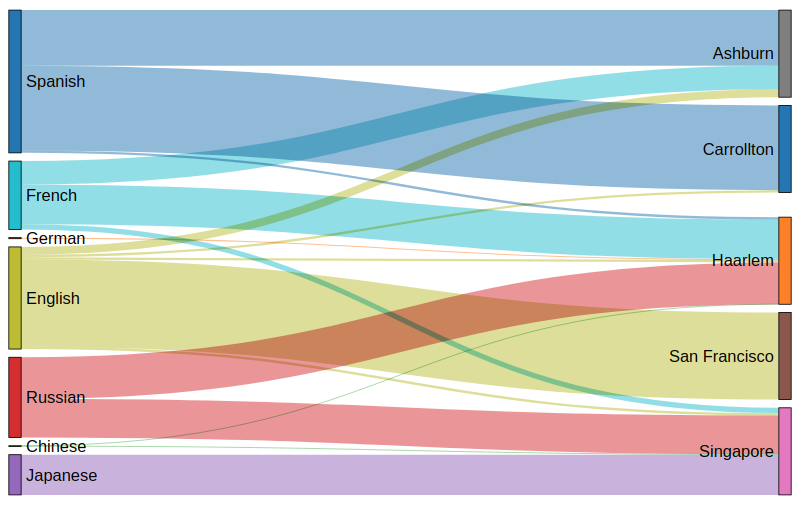
\includegraphics[scale=0.4]{embodied_cost_model/images/lang_dc_sankey.png}
    \caption[Language to Data Center Site Sankey Diagram]{Language to data center flows. The thickness of the links at each data center site indicate the relative portion of traffic that the respective language demands at the data center.}
    \label{land_dc_sankey}
    \end{figure}
    
    \subsection{System Boundary}
    The presented framework is intended to be used as a tool in data center life cycle assessments (LCA), where prevalent LCA practices are followed. In standard practice, product specific LCA studies generally entail four phases: 1) goal and scope phase, 2) the inventory analysis phase, 3) the impact assessment phase, and 4) the interpretation phase \cite{ISO14040}. The methodology, data sets, and software tools presented in the research is conducive for the first three LCA phases which all require quantitative assessment of data center environmental footprints. Stated more explicitly, this research’s goal is to provide a model that can be used to quantify the energy and carbon footprint of data center systems encompassing the embodied and operational phases in a single workflow. 
    
    Figure~\ref{system_boundary} illustrates the boundary conditions the boundary conditions with in the scope of this framework. In the scope are for paths of input of raw materials and energy from the ecosphere. Two paths lead to the embodied systems found in data centers; building construction and information technology manufacturing. While the other two path lead to the operational systems that are required to run the data centers. 
    
    \begin{figure}[h!]\centering
    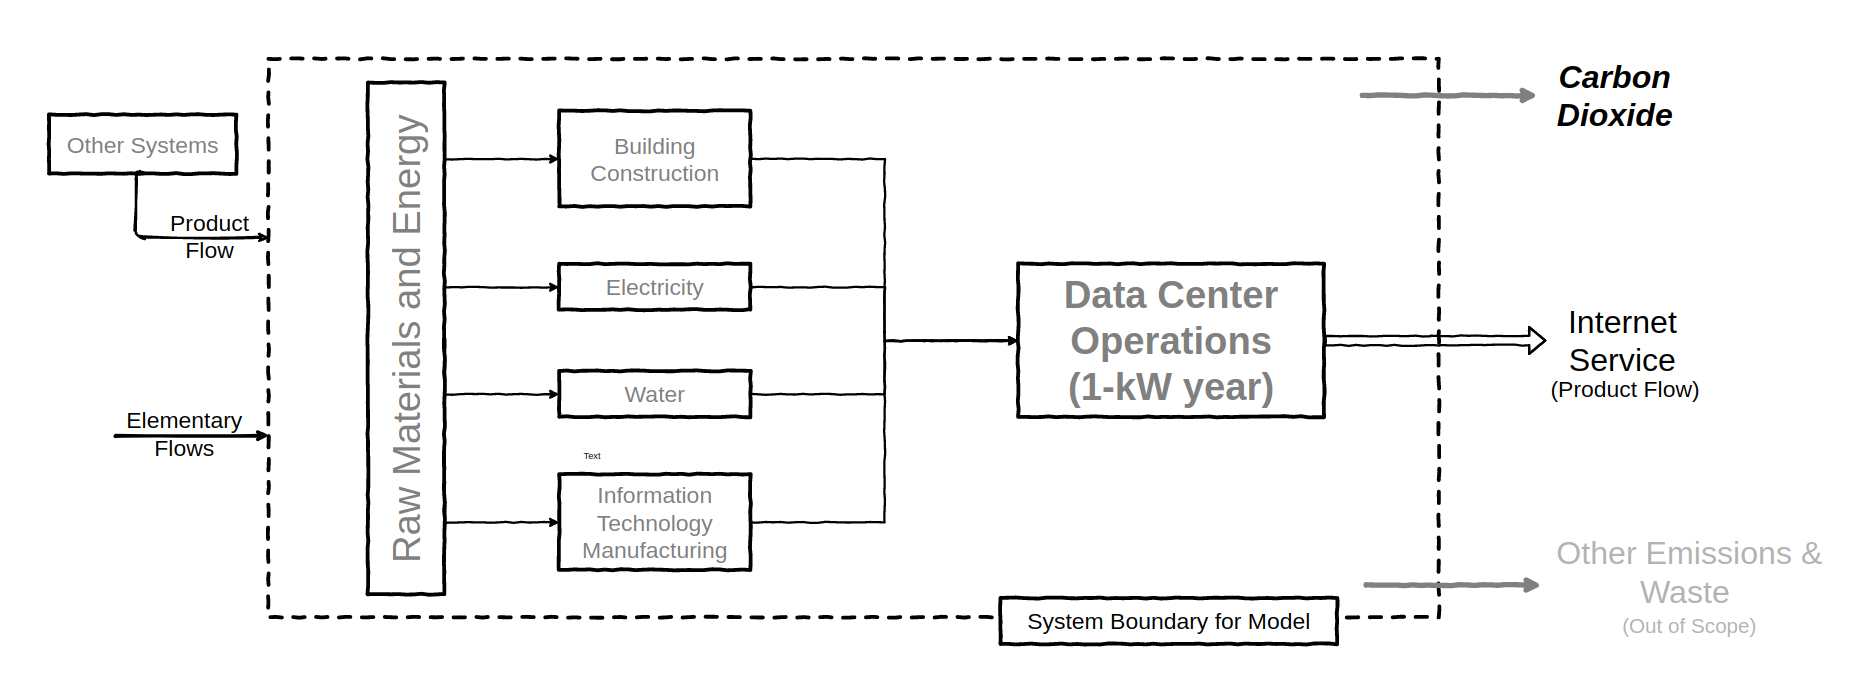
\includegraphics[scale=0.25]{embodied_cost_model/images/system_boundary2.png}
    \caption[System Boundary Diagram]{System Boundary for 1-kW of Provisioned Data Center Capacity.}
    \label{system_boundary}
    \end{figure}
    
    The geographical bounds of the service are illustrated in Figure~\ref{image:world_language_map}. The map indicates the countries in which each language from the Wikipedia set are the official languages. From  Figure~\ref{land_dc_sankey} it can be seen that one or more languages can be supported at a single data center facility. Although the workloads originate across international boundaries, the environmental emissions studied in this research are attributed to the data center sites only.  
    
    \definecolor{chinese}{rgb}{0, 1, 0} %chinese 
\definecolor{english}{rgb}{0, 0, 1}%english 
\definecolor{french}{rgb}{.8, 0, 0}%french 
\definecolor{german}{rgb}{.5, .5, .5}%german 
\definecolor{japanese}{rgb}{0, 0, .5}%japanese 
\definecolor{russian}{rgb}{0, .5, 0}%russian 
\definecolor{spanish}{rgb}{0, .25, .5}%spanish 


\begin{figure}[h]
\centering

        \begin{tikzpicture}
        \begin{scope}[xshift=1.5cm]
            \node[anchor=south west,inner sep=0] (image) at (0,0)
            {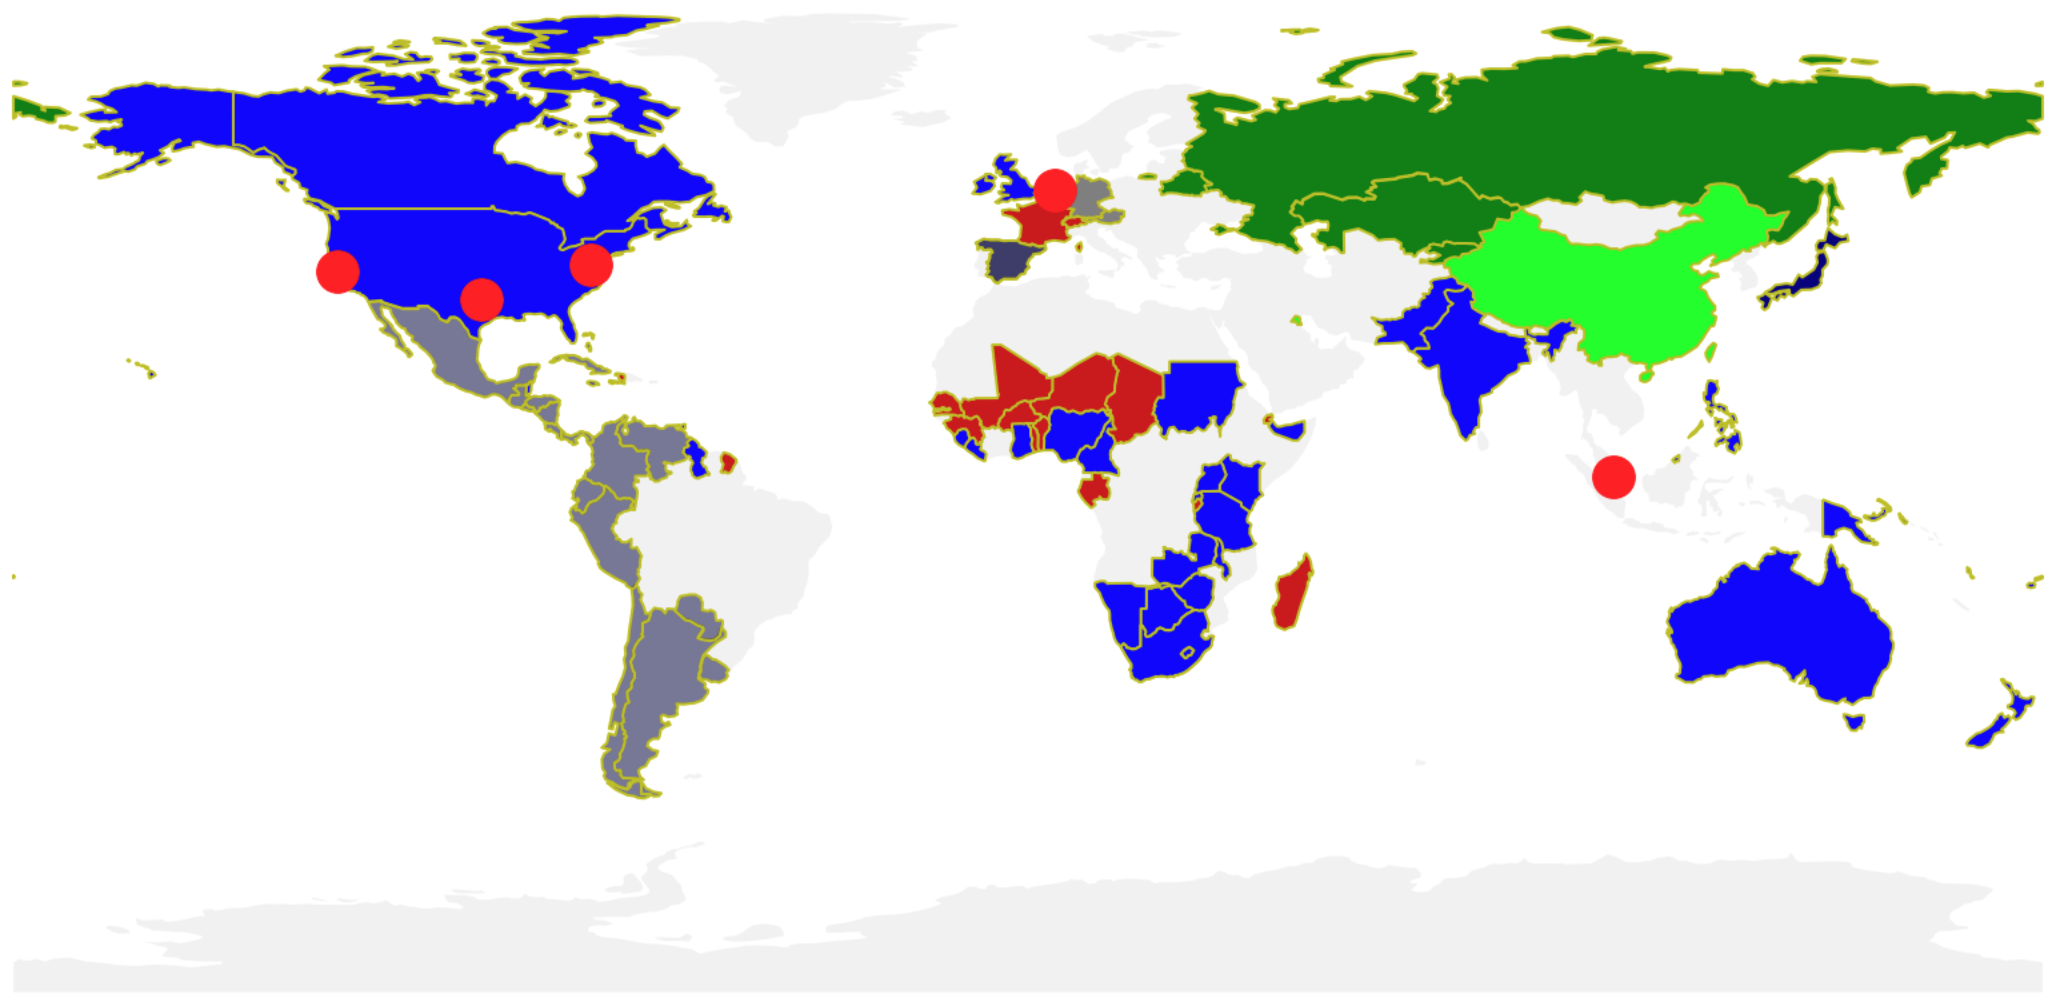
\includegraphics[width=1\textwidth]{embodied_cost_model/images/world_language_map_3.png}};
        \end{scope}
        
        \begin{scope}[xshift=1.0cm]
            \node [anchor=center] (chinese) at (2,-.6) {\small{Chinese}};
            \filldraw[outer color=chinese, inner color=chinese] (1.8,-.4) rectangle (2.2,0); % chinese
            
            \node [anchor=center] (english) at (4,-.6) {\small{English}};
            \filldraw[outer color=english, inner color=english] (3.8,-.4) rectangle (4.2,0); % english
            
            \node [anchor=center] (french) at (6,-.6) {\small{French}};
            \filldraw[outer color=french, inner color=french] (5.8,-.4) rectangle (6.2,0); % french
            
            \node [anchor=center] (german) at (8,-.6) {\small{German}};
            \filldraw[outer color=german, inner color=german] (7.8,-.4) rectangle (8.2,0); % german
            
            \node [anchor=center] (japanese) at (10,-.6) {\small{Japanese}};
            \filldraw[outer color=japanese, inner color=japanese] (9.8,-.4) rectangle (10.2,0); % japanese
            
            \node [anchor=center] (russian) at (12,-.6) {\small{Russian}};
            \filldraw[outer color=russian, inner color=russian] (11.8,-.4) rectangle (12.2,0); % russian
            
            \node [anchor=center] (spanish) at (14,-.6) {\small{Spanish}};
            \filldraw[outer color=spanish, inner color=spanish] (13.8,-.4) rectangle (14.2,0); % spanish
            
            \node [anchor=center] (dc_location) at (9,-1.1) {\small{Data Center Locations}};
            \filldraw[red] (7,-1.1) circle (4pt); 
            
            \end{scope}
            
        \end{tikzpicture}

\caption[Source country of language and DC locations]{Source country of language and DC locations map.}
\label{image:world_language_map}
\end{figure}
    
    Within these data center sites, specific sub-systems are segregated as listed in Table~\ref{tab:dc_subsystem_boundaries}. Demarcation by these sub-systems allows development of the embodied and operational models to align with industrial cost breakdown data and in terms of EIO industrial vectors. Table~\ref{tab:dc_subsystem_boundaries} serves the structural backbone for all the models developed in this framework as discussed next.
    
    \begin{table}[h]
\centering
\begin{tabular}{|l|l|} \hline
\bf{System Boundary} & \bf{Examples} \\ \hline 
Building Systems & Data Center Shell and Core \\ \hline
Cooling Systems & Air Handling Units and hydronic plants \\ \hline
Power Distribution & UPS, PDU, Cables, Diesel Generators \\ \hline
Information Technology & Compute, Storage, Network \\
\hline\end{tabular}
\caption{Sub System Boundaries}
\label{tab:dc_subsystem_boundaries}
\end{table}
    
    \subsection{Operational Inventories}
    
    \comment{The functional unit is not tied with the operational energy. The result maybe something like $\frac{kWh}{kw}$ (?) the lower the the number the more adverse it will be. Also this can be relative factor; i.e 1 for kWh*8760 hours, with kWh - kW capacity.}
    
    In this section, this research's methodology to assess the operational energy and carbon footprint of data center site infrastructure is presented. There are extensive theoretical data center energy use models in literature \cite{dayarathna16, joshi12}. These models can generally be segregated between IT and building systems domains. The model developed in this research couples the two domains by first selecting the the right IT component to model; i.e. the IT component that the total energy of the data centers is most sensitive to.
    
    Detailed industrial power usage insights are lacking in the public domain \cite{Masanet20}. As an exception some industrial insights are provided by Barroso in \cite{barroso18, barroso13}. Barroso provides Google's distribution of power for various points-of-use as indicted by the pie-charts shown in Figure~\ref{fig:power_dist_pies} for two generations of technology. In 2012, more than 80\% of the energy in a data center was used by four components; CPU 42\%, Cooling 15.4\%, disk 14.3\% and DRAM 11.7\%. By 2017, the cooling overhead had decreased to only account for 3\% a data center energy use, this decrease in cooling inflated the relative fraction of CPU and DRAM energy requirement. From these distributions, it is apparent that CPU's power usage is the dominant hot-spot.  
    
    \definecolor{pistachio}{rgb}{0.58, 0.77, 0.45} %cpu
\definecolor{denim}{rgb}{0.08, 0.38, 0.74} %dram
\definecolor{babyblue}{rgb}{0.54, 0.81, 0.94} % disk/hdd
\definecolor{azure}{rgb}{0.0, 0.5, 1.0} % storage
\definecolor{chartreuse}{rgb}{0.5, 1.0, 0.0} % nw
\definecolor{ashgrey}{rgb}{0.7, 0.75, 0.71} % balance/misc
\definecolor{bananamania}{rgb}{0.98, 0.91, 0.71} % psu
\definecolor{citrine}{rgb}{0.89, 0.82, 0.04} % power dist
\definecolor{cinnabar}{rgb}{0.89, 0.26, 0.2} %cooling

\begin{figure}[h]
\centering

\begin{tikzpicture}

% specify the pie charts
\node [anchor=center] (mix-ssd) at (0,3.5) {Power Allocation in 2012 \cite{barroso13}};
\pie[explode={0, 0, 0, 0}, , radius = 3, text=hide,color={pistachio, denim, babyblue, chartreuse, ashgrey, citrine, cinnabar }] 
{42/cpu, 11.7/dram, 14.3/disk, 4.9/nw, 4/misc, 7.7/power_dist, 15.4/cooling}
\definecolor{airforceblue}{rgb}{0.36, 0.54, 0.66}
\node [anchor=center] (mix-hdd) at (7,3.5) {Power Allocation in 2017 \cite{barroso18}};
\pie[pos={7,0}, explode = 0, radius = 3, text=hide, color={pistachio, denim, azure, chartreuse, ashgrey, citrine, cinnabar }] {60.6/cpu, 17.9/dram, 2.0/storage, 5.0/nw, 4/misc, 7.6/power_dist, 3.0/cooling}

%Specify the legend
\node [anchor=east] (cpu) at (-2,-3.8) {\small{CPU}};
\filldraw[outer color=pistachio, inner color=pistachio] (-2,-4) rectangle (-1.6,-3.6); % cpu

\node [anchor=east] (storage) at (0,-3.8) {\small{DRAM}};
\filldraw[outer color=denim, inner color=denim] (0,-4) rectangle (0.4,-3.6); % dram

\node [anchor=east] (disk) at (1.8,-3.8) {\small{Disk}};
\filldraw[outer color=babyblue, inner color=babyblue] (1.8,-4) rectangle (2.2,-3.6); % disk

\node [anchor=east] (psu) at (4,-3.8) {\small{Storage}};
\filldraw[outer color=azure, inner color=azure] (4,-4) rectangle (4.4,-3.6); %nw

\node [anchor=east] (balance) at (6.2,-3.8) {\small{Balance}};
\filldraw[outer color=ashgrey, inner color=ashgrey] (6.2,-4) rectangle (6.6,-3.6); % balance

\node [anchor=east] (power) at (10,-3.8) {\small{Power Distribution}};
\filldraw[outer color=citrine, inner color=citrine] (10,-4) rectangle (10.4,-3.6); % power dist

\node [anchor=east] (cooling) at (2,-4.6) {\small{Cooling}};
\filldraw[outer color=cinnabar, inner color=cinnabar] (2,-4.8) rectangle (2.4,-4.4); %cooling

\node [anchor=east] (nw) at (6,-4.6) {\small{Network}};
\filldraw[outer color=chartreuse, inner color=chartreuse] (6,-4.8) rectangle (6.4,-4.4); %nw

\end{tikzpicture}

\caption[Barroso's Power Distribution]{Data Center Power Distribution for Two Generation of Technology}
\label{fig:power_dist_pies}
\end{figure}
    
    The values in Figure~\ref{fig:power_dist_pies} are annualized distributions. In practice the power demand of data centers is very dynamic and sensitive to complex workload dependencies. These dependencies lend themselves to be exploited in power proportional computing paradigms. Several proportional workload techniques are discussed in detail by O'Sullivan in \cite{osullivan15}. This research takes such techniques and extends building energy models to be aware of proportional CPU loads based on coming network traffic to a data center site.
    
    Specifically, the embodied costs of the data center materials are extended to the EnergyPlus model from Chapter~\ref{chp:bem}. EnergyPlus provides a comprehensive indication of the operational energy and together with the marginal cost of energy model from Chapter~\ref{chp:mec}, it exposes the carbon footprint for each of the five data centers and the language abstracted service pairs. Both models are based on the network coefficients  from Chapter~\ref{chp:traffic}. The traffic coefficients are used to reset the IT workloads at each data centers and the marginal costs to produce energy in the regional grid. The details of the models is indicated in Algorithm~\ref{mec_coupled_bem_algo} and the general framework is illustrated in Figure~\ref{process_flow}.
    
      \begin{algorithm}

    \caption{MEC coupled BEM algorithm}
    \begin{algorithmic}
      \REQUIRE $DOSCOE[region_i]$ \& $traffic.language[site_{DC}]$
      \FOR{site and region in $DC.site$ and $DC.region$}
        \IF{traffic.language[site].all $!= 0$: }
        \STATE $D_{DC} \gets BEM(site, traffic.language[site_{DC}])$
        \STATE $DOSCOE[region].demand  \mathrel{+}=  D_{DC}$
        \ENDIF
      \ENDFOR
      \RETURN $CO_{2}$ {footprint}$\ =\ GridSim(region, rps)$
      
      \begin{small}
      \vspace{.1in}
      \STATE{\bf{Where}}: \\
     
        \hspace{.2in} $DOSCOE[region_i]$ = Dispatch Optimized System Cost of Energy Model for $region_i$ \cite{platt17}.  \\
        \hspace{.2in} $site_{DC}$ = data center site. \\
        \hspace{.2in} $traffic.language_l[site_{DC}]$ = the traffic routed to data center for lanuage $l$.  \\
        \hspace{.2in} $DC.site$ = list of all data centers in the network. \\
        \hspace{.2in} $DC.region$ = list of corresponding power grid region for the data centers in $DC.site$ . \\
        \hspace{.2in}$DOSCOE[region].demand$ = demand vector of loads added to the power grid for every hour. \\
        \vspace{.1in}
        \STATE{\bf{External Models}}: \\
        \vspace{.05in}
        \hspace{.2in}{$BEM(site, traffic.language[site_{DC}])$ is a EnergyPlus model of the data center. As an external argument the traffic profile for the language to the data center is passed. The traffic profiles serve as coefficients for the IT load, bounded by 0 and 1.  The output is a vector indicating the building energy demands for each hour of the year.} \\
        \vspace{.05in}
        \hspace{.2in}$GridSim(region, rps)$ is a DOSCOE model with $DOSCOE[region].demand$ and renewable portfolio standard ($rps$) value indicating the required penetration percentage of renewable energy in the power supply. The model quantifies the costs of energy in terms of carbon footprint and monetary values. 
        \end{small}
    \end{algorithmic}
    \label{mec_coupled_bem_algo}

  \end{algorithm}
    
    \begin{figure}[h]
\centering
\begin{tikzpicture}
% \node [anchor=west] (scope) at (8.75,5.5) {Embodied Costs};
\node [anchor=west] (embodied) at (9.6,-.3) {(Scope of Chapter)};
% \node [anchor=west] (traffic) at (1.4,5.5) {Traffic};
% \node [anchor=west] (bem) at (4.2,5.5) {BEM};
% \node [anchor=west] (mec) at (6.75,5.5) {MEC};
\begin{scope}[xshift=1.5cm]
    \node[anchor=south west,inner sep=0] (image) at (0,0) {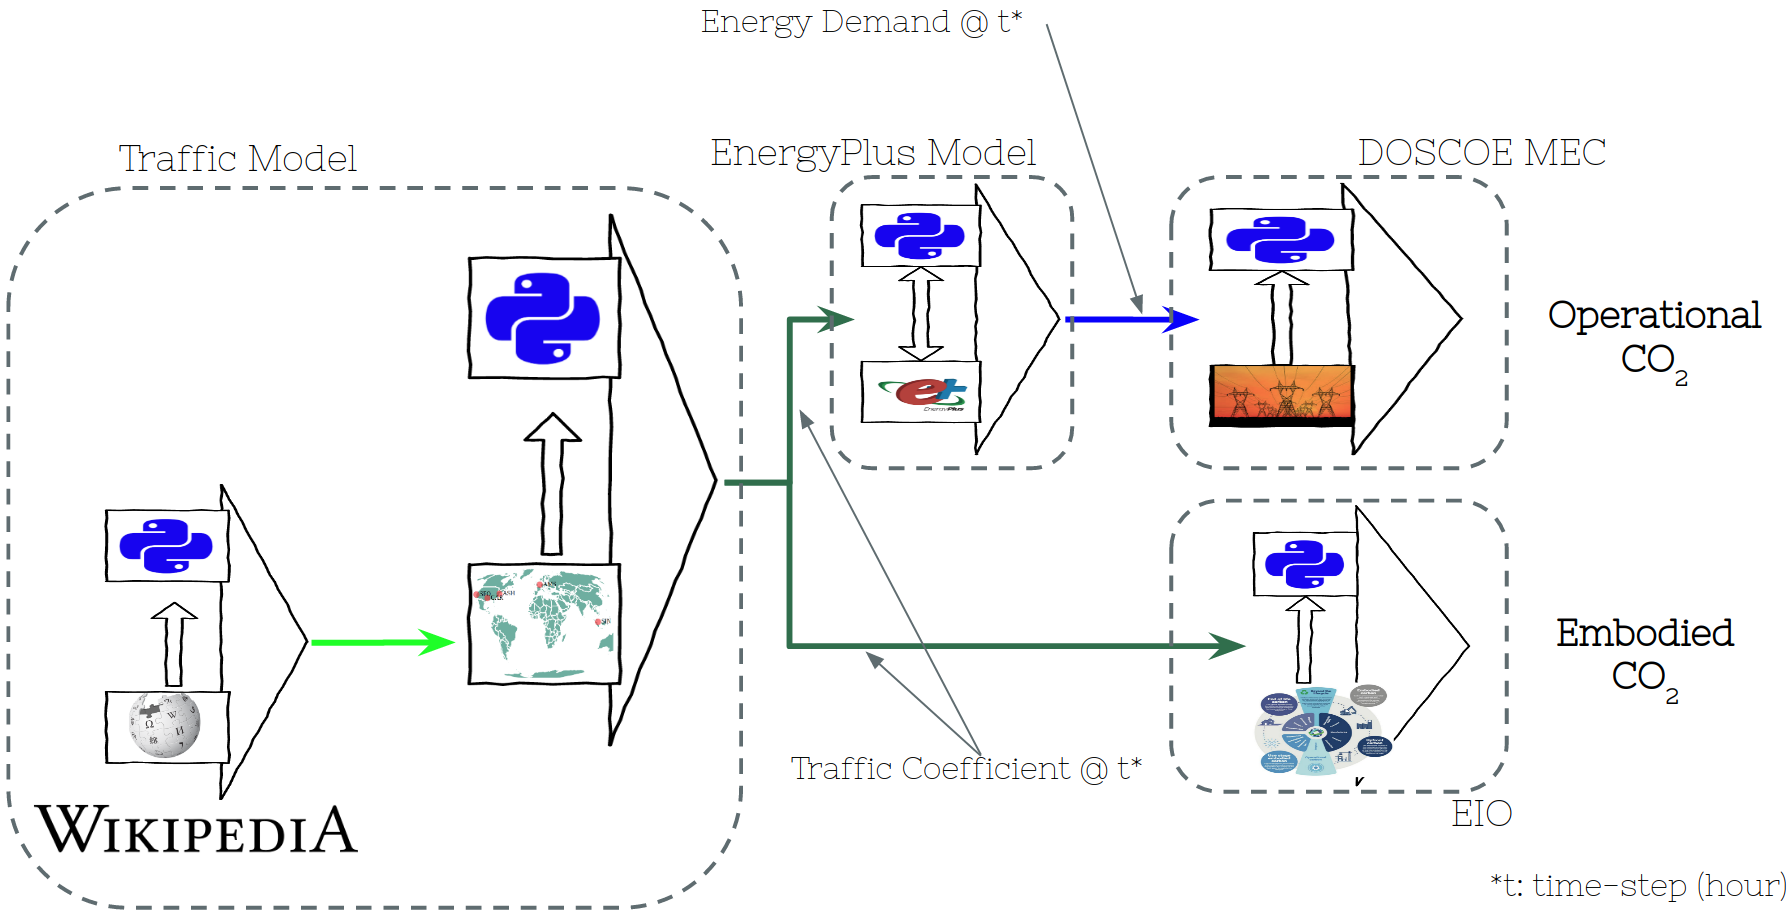
\includegraphics[width=0.8\textwidth]{embodied_cost_model/images/horizontal_process_flow2.png}};
    \begin{scope}[x={(image.south east)},y={(image.north west)}]
        \draw[ultra thick,rounded corners, ,dashed] (0.625,0.90) rectangle (1.05,0..08);
        % \draw [-stealth, line width=5pt, cyan] (scope) -- ++(0.6,0.0);
    \end{scope}
\end{scope}
\end{tikzpicture}
\caption[Model Process Flow Diagram]{Model Process Flow Diagram.}
\label{process_flow}
\end{figure}
    
    \subsection{Embodied Inventories}
    Embodied cost assessments account for the natural resources consumed when extracting, transforming, manufacturing, transporting, constructing, maintaining, and disposing the product under study. The first step in these assessments is to set the boundary conditions of the system. The second step is to select the method of the assessment. Two methods are available for such assessment; namely process based or EIO based. Process based methods are bottoms up procedures; accounting for all processes that are required to transform raw materials into consumer goods. However in process based methods as the product boundary and the count of processes to quantify can have exponentially correlations. This exponential growth can become an intractable task for building designers. A more tractable method is the EIO, where economic relationships between two industries at the national level are exploited. . 
    
    Leontief's original use case of the EIO was to identify the contribution from all economic sectors required to produce a unit of specific products in an economy.  The formulation of Leontief's EIO is indicated by Equation~\ref{eq:Leontief_IO}; where $Y$ is the input costs, $I$ is the identity matrix, and $A$ is the direct costs array \cite{matthews15}. In general direct costs represent the entire economy as a two-dimensional square array, where the rows and columns indicate distinct sectors within the economy. The values in the array indicate the row-index-sector’s input into the column-header-sector. Since their development in the 1930's, EIOs have been commonly used to characterize national economic accounts. More recently, Matthews and Hendrickson showed that EIO can be used for environmental life cycle assessments as-well \cite{matthews15}.  
    
        \begin{equation} \label{eq:Leontief_IO}
        [I-A]^{-1}Y
        \end{equation}
   
    Due to the streamlined approach of the EIO method compared to process based environmental assessments methods, the former is preferred for this research. Specifically, the United States Environmentally Extended Input-Out (USEEIO) model developed by Yang for the EPA is used in this research \cite{yang17}. The USEEIO’s economic relationship between sectors is based on 2007 cost data, while the environmental data are derived from 2013 emissions data. Both were the most up-to-date data available to the researchers at their time of publication. They suggest using 2013 cost of money for inputs, having demonstrated that the underlying structure of the economy has not shifted significantly between 2007 and 2013. 
    
        \subsubsection{Building Systems}
        Typically, data center shells and structural cores are under the jurisdiction of the same building codes as other commercial buildings, i.e. Type IIA construction types. However, the dense population of computers along with the  power and cooling requirements of data centers make several things clearly distinguishable from most commercial building types. The differences are significant enough to make the generic building sector's USEEIO environmental inventories invalid for data centers. 
        
        To more accurately represent data center buildings, several general contractor proposals for new data center construction and retrofit projects were reviewed for the cost distribution of the trades labor and equipment costs.  The contractor cost allocations per trade divisions were then compared with the values of the handful of building construction sectors available in the USEEIO. Based on the comparisons, the USEEIO manufacturing buildings sector is found to be the most similar for data centers. However, there are still shortfalls between data centers and the manufacturing buildings sector. To overcome the shortfalls, a hybrid method was used to construct a more representative Y vector for data centers. 
        
        The resulting Y vector for the building and building utilities systems is shown in Table~\ref{tab:eeio_y_building_table}. The table indicates the cost input required to provision a functional unit of 1 kW of data center capacity. Each sector's cost is derived from the contractor costs for the corresponding construction specification division as listed  in their proposals. Seven explicit sectors are quantified in addition to the manufacturing building sector. The manufacturing building/us is a catch all sector. This sector catches all the building trades that are not represented by the other entries in the Y vector; such as concrete or steel. 
        
        \begin{table}[h]
\centering
\begin{tabular}{|l|l|l|} \hline

\bf{ID} & \bf{Sector Name} & \bf{\$/kW}  \\ \hline

333415 & air conditioning, refrigeration, and heating equipment/us & 550 \\ \hline
333611 & turbines and turbine generator sets/us & 770 \\ \hline
335311 & specialty transformers/us & 50 \\ \hline
335313 & switchgear and switchboards/us & 100 \\ \hline
335920 & communication and energy wire and cable/us & 100 \\ \hline
335999 & other miscellaneous electrical equipment and components/us & 40 \\ \hline
335314 & relay and industrial controls/us & 150 \\ \hline
233230 & manufacturing buildings/us & 5250 \\ \hline

\end{tabular}
\caption{EEIO Costs Vector for Building and Utilities Infrastructure}
\label{tab:eeio_y_building_table}
\end{table}


        
        \subsubsection{Information Technology Systems}
        
        In this subsection the IT equipment's inventories are assessed. The IT equipment in a data center can be categorized broadly into three segments: compute, storage, and network. Within each of these segments, data center operators can further tune the hardware configurations to optimize their workloads. Figure~\ref{fig:server_cost_apportionment} indicates component wise cost distribution for five hardware stock-keeping units (SKU). The SKU data were obtained under non-disclosure agreements from a large internet website operator.  
        
        \definecolor{pistachio}{rgb}{0.58, 0.77, 0.45}
\definecolor{babyblue}{rgb}{0.54, 0.81, 0.94}
\definecolor{bananamania}{rgb}{0.98, 0.91, 0.71}
\definecolor{pinkpearl}{rgb}{0.91, 0.67, 0.81}
\definecolor{ashgrey}{rgb}{0.7, 0.75, 0.71}

\begin{figure}[h]
\centering

\begin{tikzpicture}
\node [anchor=center] (mix-ssd) at (0,1.75) {SSD Server};
\pie[explode={0, 0, 0, 0}, , radius = 1.5, text=hide,color={pistachio, babyblue, pinkpearl, bananamania, ashgrey}] {72/sc, 15/hdd, 5/mbd,
4/psu, 4/balance}

\node [anchor=center] (mix-hdd) at (4,1.75) {HDD Server};
\pie[pos={4,0}, explode = 0, radius = 1.5, text=hide, color={pistachio, babyblue, pinkpearl, bananamania, ashgrey}] {58/sc, 29/hdd, 6/mbd,
4/psu, 3/balance}

\node [anchor=center] (high-op) at (8,1.75) {High-IO Server};
\pie[pos={8,0}, explode = 0, radius = 1.5, text=hide, color={pistachio, babyblue, pinkpearl, bananamania, ashgrey}] {69/sc, 16/hdd, 7/mbd,
8/psu, 6/balance}

\node [anchor=center] (compute) at (2,-2.25) {Compute Server};
\pie[pos={2,-4}, explode = 0, radius = 1.5, text=hide, color={pistachio, babyblue, pinkpearl, bananamania, ashgrey}] {48/sc, 25/hdd, 13/mbd,
8/psu, 6/balance}

\node [anchor=center] (low-mem) at (6,-2.25) {Low-Memory Server};
\pie[pos={6,-4}, explode = 0, radius = 1.5, text=hide, color={pistachio, babyblue, pinkpearl, bananamania, ashgrey}] {51/sc, 34/hdd, 6/mbd,
4/psu, 5/balance}

\node [anchor=center] (semiconductor) at (.2,-7.25) {\small{CPU, Memory,}};
\node [anchor=center] (semiconductor) at (.2,-7.6) {\small{SSD}};
\node [anchor=center] (storage) at (2.7,-7.25) {\small{Hard Disc}};
\node [anchor=center] (storage) at (2.7,-7.6) {\small{Drive}};
\node [anchor=center] (pcb) at (5.2,-7.25) {\small{Motherboard}};
\node [anchor=center] (psu) at (7.7,-7.25) {\small{Power Supply}};
\node [anchor=center] (balance) at (10.2,-7.25) {\small{Balance}};

\filldraw[outer color=pistachio, inner color=pistachio] (0,-7) rectangle (0.4,-6.6);
\filldraw[outer color=babyblue, inner color=babyblue] (2.5,-7) rectangle (2.9,-6.6);
\filldraw[outer color=pinkpearl, inner color=pinkpearl] (5,-7) rectangle (5.4,-6.6);
\filldraw[outer color=bananamania, inner color=bananamania] (7.5,-7) rectangle (7.9,-6.6);
\filldraw[outer color=ashgrey, inner color=ashgrey] (10,-7) rectangle (10.4,-6.6);

\end{tikzpicture}

\caption[Server Cost Apportionment Chart]{Cost apportionment of deployable hardware. See Table~\ref{tab:sku_cost_dist_table} for details of USEEIO sector mapping. The values are representative of deployment cost share per server during 2015 and 2016. Data acquired by author from an DC operator under NDA.}
\label{fig:server_cost_apportionment}
\end{figure}
        
        The configuration of the server SKUs are optimized for the workloads that they support. For example the High-IO server is optimized for high rates of input and outputs; where it processes information at high feed rates. As an example, this useful for workloads that require external communications with a large data set that is housed in a Mix-SSD server that has an abundance of data storage capacity. For a data center with dominant heterogeneous workloads will have a mix of of these SKUs, whereas a data center with a single workload would have only one or two distinct SKUs.
        
        The values in Figure~\ref{fig:server_cost_apportionment} are indicative of the deployment cost share per server between 2015 and 2016. Server components such as processors (CPU), memory (MEM), and solid-state-drives (SSD) are fabricated using semiconductor manufacturing processes. These components are grouped together and are categorized as a single input into the USEEIO’s semiconductor sector. Hard disc drives (HDD), motherboard (MBD), and power supply units (PSU) have representative sectors that allow a one to one mapping within the USEEIO. Other components such as chassis, thermal-heat sinks, and cable connectors are grouped into the balance category. The balance category is mapped to the generic computer sector in USEEIO. This costs apportionment values can are used to construct the Y vector for input in the USEEIO.
        
        \newcommand*\rot{\rotatebox{90}}
\newcommand*\OK{\ding{51}}

\begin{table}[h]
\vspace{-10 pt}
\centering
\scalebox{0.8}{%
\begin{tabular}{|l|l|l|l|l|l|l|} \hline

\bf{Component} & \bf{USEEIO Sector} & \rot{\bf{SSD }} & \rot{\bf{Mix-HDD }} & \rot{\bf{High-IO }} & \rot{\bf{Compute}} & \rot{\bf{Low-Mem}} \\ \hline

CPU, Memory, & semiconductors/us & 72\% & 58\% & 69\% & 48\% & 51\% \\ 
SSD &  &  &  &  &  &  \\ \hline

HDD & computer storage & 15\% & 29\% & 16\% & 25\% & 34\% \\ 
 & device readers/us &  &  &  &  &  \\ \hline
 
Motherboard & printed circuit and  & 5\% & 6\% & 7\% & 13\% & 6\% \\
 & electronic assembly/us &  &  &  &  &  \\ \hline

Power Supply  & Electronic Capacitors & 4\% & 4\% & 4\% & 8\% & 4\% \\ 
Unit & and other components &  &  &  &  &  \\
 & (except semiconductors and &  &  &  &  &  \\ 
 & printed circuit assemblies)/us &  &  &  &  &  \\ \hline
 
Balance of Parts & computers/us & 3\% & 3\% & 3\% & 6\% & 4\% \\ \hline

\end{tabular}}
\caption{Cost apportionment of deployable hardware stock keeping units (SKU)}
\label{tab:sku_cost_dist_table}
\vspace{-10 pt}
\end{table}

        \begin{table}[h]
\vspace{-10 pt}
\centering
\begin{tabular}{|l|c|c|} \hline

\bf{Component} & \bf{Power (Watts)} & \bf{Reference} \\ \hline 

3.5" HDD & 3.87 & \cite{fuchs219} \\ \hline
2.5" HDD & 0.89 & \cite{fuchs219} \\ \hline
SDD & 0.37 & \cite{fuchs219} \\ \hline
Single Socket CPU & 105 & \cite{kaggle17b} \\ \hline
Dual Socket CPU & 210 & \cite{kaggle17b} \\ \hline
Power Supply Unit & 25 & \cite{joshi12} \\ \hline
Motherboards & 40 & \cite{buildcomputers} \\ \hline
RAM & 0.375 & \cite{crucial} \\ \hline
Fans (5 per server) & 10 & \cite{buildcomputers} \\ \hline


\hline\end{tabular}
\caption{Server component power distribution}
\label{tab:it_component_power_dist_table}
\vspace{-10 pt}
\end{table}
        
          \begin{algorithm}
    \caption{IT equipment Y vector algorithm}
    \begin{algorithmic}
      \REQUIRE $P_{DC}$, $P_{i}$, and $C_i$
      \STATE $P_{S} \gets \sum\limits_{i=1}^n P_{i}$
    %   \STATE $C_{S} \gets \sum\limits_{i=1}^n C_{i}$
      \STATE $C_{ip} \gets C_i \times f_i$
      \STATE $S_\# \gets \frac{P_{DC}}{P_{S}}$
      \STATE $SC_{DC} \gets S_\# \times P_{S}$
      
      \vspace{.1in}
      \RETURN $Y \gets SC_{DC} \times C_{ip}$
      
      \vspace{.1in}
      \STATE{\bf{Where}}: \\
        \hspace{.2in}$P_{DC}$ = Provisioned Power of Data Center, (input variable) \\
        \hspace{.2in}$P_{i}$ = Power demand for component $i$ of server.  \\
        \hspace{.2in}$n$ = Number of components in the server.  \\
        \hspace{.2in}$C_{ip}$ = Provisioning cost of component $i$ \\
        \hspace{.2in}$C_i$ = Cost Apportions for server component $i$, (from Figure~\ref{fig:server_cost_apportionment}) \\
        \hspace{.2in}$f_i$ = Failure rate of component $i$\\
        \hspace{.2in}$S_\#$ = Count of servers in data center \\
        \hspace{.2in}$SC_{DC}$ = Total Server Costs for DC \\
        \hspace{.2in}$Y$ = Vector of sector wise costs for input to USEEIO
    
    \end{algorithmic}
    \label{it_y_vector_algo}
  \end{algorithm}
        
        \begin{table}[h]
\centering
\begin{tabular}{|l|r|}

\hline
                                          \bf{Sector} & \bf{Direct} \\
\hline
\hline
\n                                334111/computers/us &    1.029522 \\
\n          334112/computer storage device readers/us &    0.146600 \\
\n                          420000/wholesale trade/us &    0.068705 \\
\n  33411a/computer terminals and other computer p... &    0.083782 \\
\n                           334413/semiconductors/us &    0.063247 \\
\n  334418/printed circuit and electronic assembly/us &    0.049135 \\
\n        550000/company and enterprise management/us &    0.018676 \\
\n  33441a/electronic capacitors, resistors, coils... &    0.011519 \\
\n         541800/advertising and public relations/us &    0.001979 \\
\n                          484000/truck transport/us &    0.006023 \\
\hline
\end{tabular}

\caption{Unit input to USEEIO computers/us sector}
\label{tab: generic_computer_eeio}

\end{table}
        


    
\section{Results}
\section{Discussions}
\section{Conclusion}
\newpage
\section{Appendix}
        
% \chapter{Life-Cycle Energy and Carbon Footprint Modeling with Data Center Building Energy Models}
\label{chp:embodied_cost_model}

\section{Introduction}
    In this chapter, the aim is to quantify the end to end life cycle costs of data centers by extending the operational models developed in the previous chapters. Those operational models have provided an indication of system level energy for a network of data centers and their marginal carbon dioxide footprints. Although, the presented models are a good proxy for the environmental costs of data center operations, they don't account for the energy and carbon footprint embodied in all the materials that the data centers are composed of.

    To assess the end to end environmental impact of data centers, this chapter describes a three-step hybrid life-cycle analysis inclusive of the embodied inventories of the physical data center infrastructure. As the first step, the building energy and marginal costs of energy generation models are reviewed. These two models together provide an indication of the respective costs during the operational phase of a data center's life. Then as the second step, a life cycle modeling framework using an economic input-output (EIO) analysis model extended to environmental costs is introduced. The inputs to the EIO are constructed in this chapter based on literature reviews and the researcher's industrial experience. The final step provides a global view of the end to end assessment by presenting the energy and carbon footprint of each of the data center-language pair analyzed in the previous chapters. With the global view, the global environmental costs of a discrete service can be assessed.

    \subsection{Motivations for an end to end life cycle cost model}
        In terms of scale, US data centers consumed 700 billion kWh in 2016. That was 1.8\% of the total electricity produced in the country according to a United States Department of Energy (DOE) report \cite{Shehabi16}. To drive further intuition of their scale, a typical 100-MW data center at peak load consumes the same amount of energy in an hour as 100 homes do in a month. Given a data centers power demands, it is not surprising that operational energy use has a high sensitivity towards their total cost of ownership (TCO); making it a key metric in TCO based design decisions. While optimization for use phase energy may significantly reduce the carbon footprint of a data center (given the source energy mix does not change), it does not account for other phases in the data center's end to end life cycle. Inventories from embodied life cycle phases such materialization, transit, maintenance, and end of life are left out of the operational phase energy models that have become prevalent indicator of data center sustainability. 

        There are two predominant paradigms for evaluating the embodied environmental inventories for any product that has been altered by technology (techno-sphere). The first method is process based. The complexity of a process-based model is greatly influenced by the boundary conditions of the study. If the boundary is demarcated between the biosphere and the techno-sphere, then the number of distinct life cycle processes to quantify explodes by 500 times for a simple pen \cite{shah11}. The alternate method is based on Leontief's macro-economic proxies that exploits economic correlations between industrial sectors. In macro-economic models, a matrix with rows and columns equal to the number of sectors in the economy is populated with the cost relationship between the row-sector and the corresponding column-sector. Industrial-sector macro-economic proxies reduce the problem space significantly as only one cost vector is required as input to analyze an entire economy. This research combines the two paradigms and presents a hybrid life-cycle assessment model of data centers that can be used to support data center design decisions. 

        The structure of the paper is as follows. First, some technical background about data centers is provided along with a synthesis of similar works. Then in the methodology section a dynamic model to quantify the operational and embodied costs of data center infrastructure is described. The results from the methods as then presented in the results section. This article concludes by summarizing its findings and suggesting the future direction in this area of research. 

\section{Background}
    \subsection{Technical Overview of Data Centers}
        Modern internet data centers are district scale systems, spanning campuses that are hundreds of acres. They may contain several hundred thousand pieces of information technology (IT) equipment. IT equipment consists of physical servers, network hardware nodes, and digital storage media. Theses pieces of IT equipment sit alongside the data center's district scale cooling and electrical distribution plants housed in warehouse-scale built environments. The environmental footprint of a data center spans the full breadth of these physical pieces of infrastructure. 

        At their scale data centers receive power through medium voltage connections with the local utility's grid. The alternating-current voltage may then be stepped down in several steps, but ultimately, it is rectified to be used by the sensitive electronic components in the information technology hardware. Each step-down is a point of power inefficiency, with the alternating-current to direct-current conversion being the biggest point of power loss. Furthermore, anywhere that the step down or conversion occurs inside the building, the electrical inefficiencies are manifested as heat.  

        The heat from the electrical inefficiencies, along with the heat emitted by the IT equipment transistor state transitions and their current leakage, must be rejected to the outside of the building space by mechanical means. At a fundamental level, a mechanically driven fluid mover is needed to convey the heat from indoors to outdoors or another reservoir. In single pass cooling systems fans intake outside-air and force them through the IT equipment, capturing any heat and carrying it outside of the buildings. More complex cooling systems may include liquid or gas refrigerant medium thermodynamic cycles between the buildings and reservoirs, with the refrigerant medium capturing heat at either the building room level or at the scale of IT equipment. Precise modeling of such data center building systems with intense therm-power dynamics is now a manageable task in building energy modeling software \cite{kumar20,kumar20b}. 

        The embodied costs of IT equipment and building systems yield additional environmental costs for a data center's life cycle. The rate of innovation for IT equipment and the ever-increasing demands from the software applications creates a capital market where TCO of one generation of IT hardware rapidly increases relative to newer IT hardware solutions. The capital of cost/performance trade-off makes the positive TCO life of IT equipment between two to five years as observed by Shehabi in the DOE report \cite{Shehabi16}. This relatively short lifetime of IT further compounds the embodied costs of data centers. For example, through a 20-year data center building life, four to ten generations of IT transit through the facility. Disparities in lifetimes and dimensional scale differences between buildings and microchips make data center embodied inventory modeling complex. However, recently hybrid life cycle assessment models have shown to be effective in quantifying the embodied costs of data centers \cite{shah11, whitehead15}. 

        Information technology equipment requires some further insights in order to make its impact to data center life cycle analysis more concrete and directed in scope. At the heart of information technology equipment are microprocessor chips. Modern chips are composed of billions of transistors which have been getting smaller in size since their first applications in electronics signal processing in the 1960's. Transistors have been the key enabler for the compaction and power efficiency gains of electronic devices over the years and they've also been shown to have one of the most dominant environmental costs within electronic products \cite{boyd09, alcaraz18}.

        Prior to the mid-2010's, transistors were composed of planar or 2-D architectures. 2-D transistors inherently had limited operational power efficiencies due to higher voltage and current leakage compared to the novel 3-D processors in the market today. Specifically it's the 3-D processes that have allowed significant operational efficiency gains for data centered operators, yet studies assessing the 3-D transistor architecture's impact to data center life cycle costs are lacking. The 2-D to 3-D transition is a recent example of rapid rate of adaption for information technology equipment that make generalized environmental impacts studies for transducer technology obsolete in two to three years \cite{murphy03}. The frequent churn of technology also drives rapid changes in the manufacturing process of the chips. These rapid changes in semiconductor-manufacturing processes necessitates a parametrically scalable framework where transistor chips can be evaluated in isolation from other server components.  

    \subsection{Similar Works}
        In this section similar works that have quantified the environmental foot print of data centers are presented. Data center life cycle assessment works come from industrial operators \cite{shah11},  academia \cite{whitehead15,kline16}, federal agencies \cite{CLEER13}, and industrial consortium's \cite{tgg12}. Two of the reviewed works are conducive to replicate from the ground up \cite{shah11,whitehead15}, while another serves as a guideline \cite{tgg12}, and another provides an online interactive tool to assess the footprint of targeted classes of Cloud services \cite{CLEER13}. 

        From the operators perspective Shah, demonstrates an end to end life cycle assessment of data center systems \cite{shah11}. Shah uses a hybrid model inclusive of process based and economic input/output assessment frameworks to assess a single a data center, while using a static model for use-phase power. Whitehead, extends Shah's hybrid work and demonstrates the life-cycle costs of a real data center and sets an explicit functional unit of 1-kW of provisioned capacity \cite{whitehead15}.  
        
        The recent focus on product operational energy efficiency motivated Kline’s study of the trade-offs between operational energy and the embodied costs of information technology equipment \cite{kline16}. Although their bases for the embodied costs are process based, their literature does not provide sufficient insight for others to reproduce the work. Similarly, The Green Grid's Data Center Life Cycle costs guidelines outline the end goal of a data center life cycle analysis. It classifies several key attributes that need to be considered, but lacks references to explicit procedures that must be followed to achieve the goals. 
        
       The Cloud Energy and Emissions Research (CLEER) Model provides a browser based user interface to compare the environmental costs of on-premise server based services with hypothetical cloud-based systems that would provide an equivalent service \cite{CLEER13}. CLEER's analysis is transparent and inclusive of embodied and operational costs, but it does not dynamically couple the embodied or operational costs into the model. The presented set of past works has inspired the methodology of this research as described in the next section.

\section{Methodology}
    \subsection{Functional Unit and Reference Flows}
    Life cycle assessment studies require a functional unit of performance of the system under study for use as a normalized reference point. As a reference point for data centers, there is an industry wide consensus that power is the best indicator for a data center's workload capacity \cite{shah11, whitehead15, barroso18}. Based on the consensus, the functional unit adapted for this research is chosen to be 1-kW of provisioned power per year. 
    
    Furthermore, for the abstracted functional unit to be used in comparisons between different data center design scenarios requires it to be translated to reference flow values. In this work the reference flow is constrained to 1-year of data center operations with the globally provisioned power footprint of each of the language abstracted internet services. The language (internet service) to data center distribution is indicated in Figure~\ref{land_dc_sankey}. 
    
    \begin{figure}[h!]\centering
    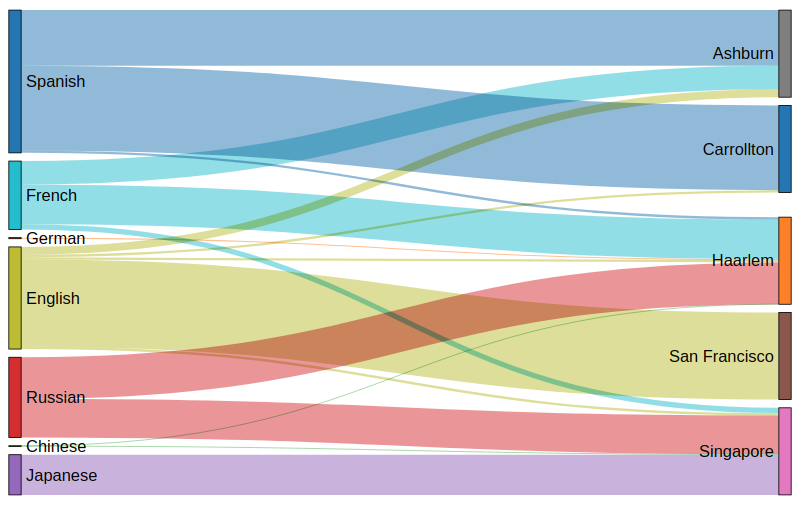
\includegraphics[scale=0.4]{embodied_cost_model/images/lang_dc_sankey.png}
    \caption[Language to Data Center Site Sankey Diagram]{Language to data center flows. The thickness of the links at each data center site indicate the relative portion of traffic that the respective language demands at the data center.}
    \label{land_dc_sankey}
    \end{figure}
    
    \subsection{System Boundary}
    The presented framework is intended to be used as a tool in data center life cycle assessments (LCA), where prevalent LCA practices are followed. In standard practice, product specific LCA studies generally entail four phases: 1) goal and scope phase, 2) the inventory analysis phase, 3) the impact assessment phase, and 4) the interpretation phase \cite{ISO14040}. The methodology, data sets, and software tools presented in the research is conducive for the first three LCA phases which all require quantitative assessment of data center environmental footprints. Stated more explicitly, this research’s goal is to provide a model that can be used to quantify the energy and carbon footprint of data center systems encompassing the embodied and operational phases in a single workflow. 
    
    Figure~\ref{system_boundary} illustrates the boundary conditions the boundary conditions with in the scope of this framework. In the scope are for paths of input of raw materials and energy from the ecosphere. Two paths lead to the embodied systems found in data centers; building construction and information technology manufacturing. While the other two path lead to the operational systems that are required to run the data centers. 
    
    \begin{figure}[h!]\centering
    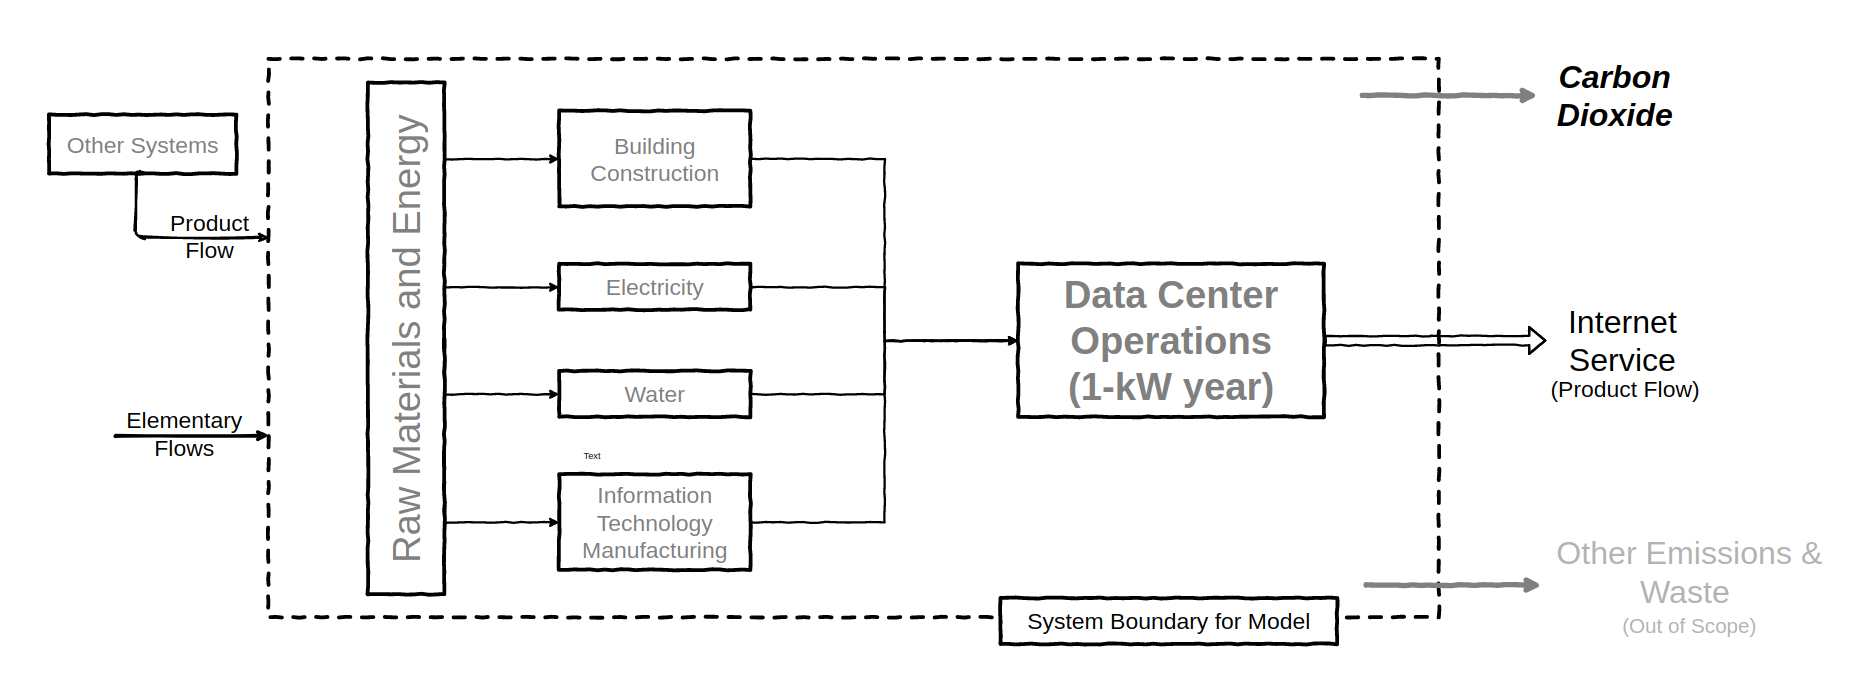
\includegraphics[scale=0.25]{embodied_cost_model/images/system_boundary2.png}
    \caption[System Boundary Diagram]{System Boundary for 1-kW of Provisioned Data Center Capacity.}
    \label{system_boundary}
    \end{figure}
    
    The geographical bounds of the service are illustrated in Figure~\ref{image:world_language_map}. The map indicates the countries in which each language from the Wikipedia set are the official languages. From  Figure~\ref{land_dc_sankey} it can be seen that one or more languages can be supported at a single data center facility. Although the workloads originate across international boundaries, the environmental emissions studied in this research are attributed to the data center sites only.  
    
    \definecolor{chinese}{rgb}{0, 1, 0} %chinese 
\definecolor{english}{rgb}{0, 0, 1}%english 
\definecolor{french}{rgb}{.8, 0, 0}%french 
\definecolor{german}{rgb}{.5, .5, .5}%german 
\definecolor{japanese}{rgb}{0, 0, .5}%japanese 
\definecolor{russian}{rgb}{0, .5, 0}%russian 
\definecolor{spanish}{rgb}{0, .25, .5}%spanish 


\begin{figure}[h]
\centering

        \begin{tikzpicture}
        \begin{scope}[xshift=1.5cm]
            \node[anchor=south west,inner sep=0] (image) at (0,0)
            {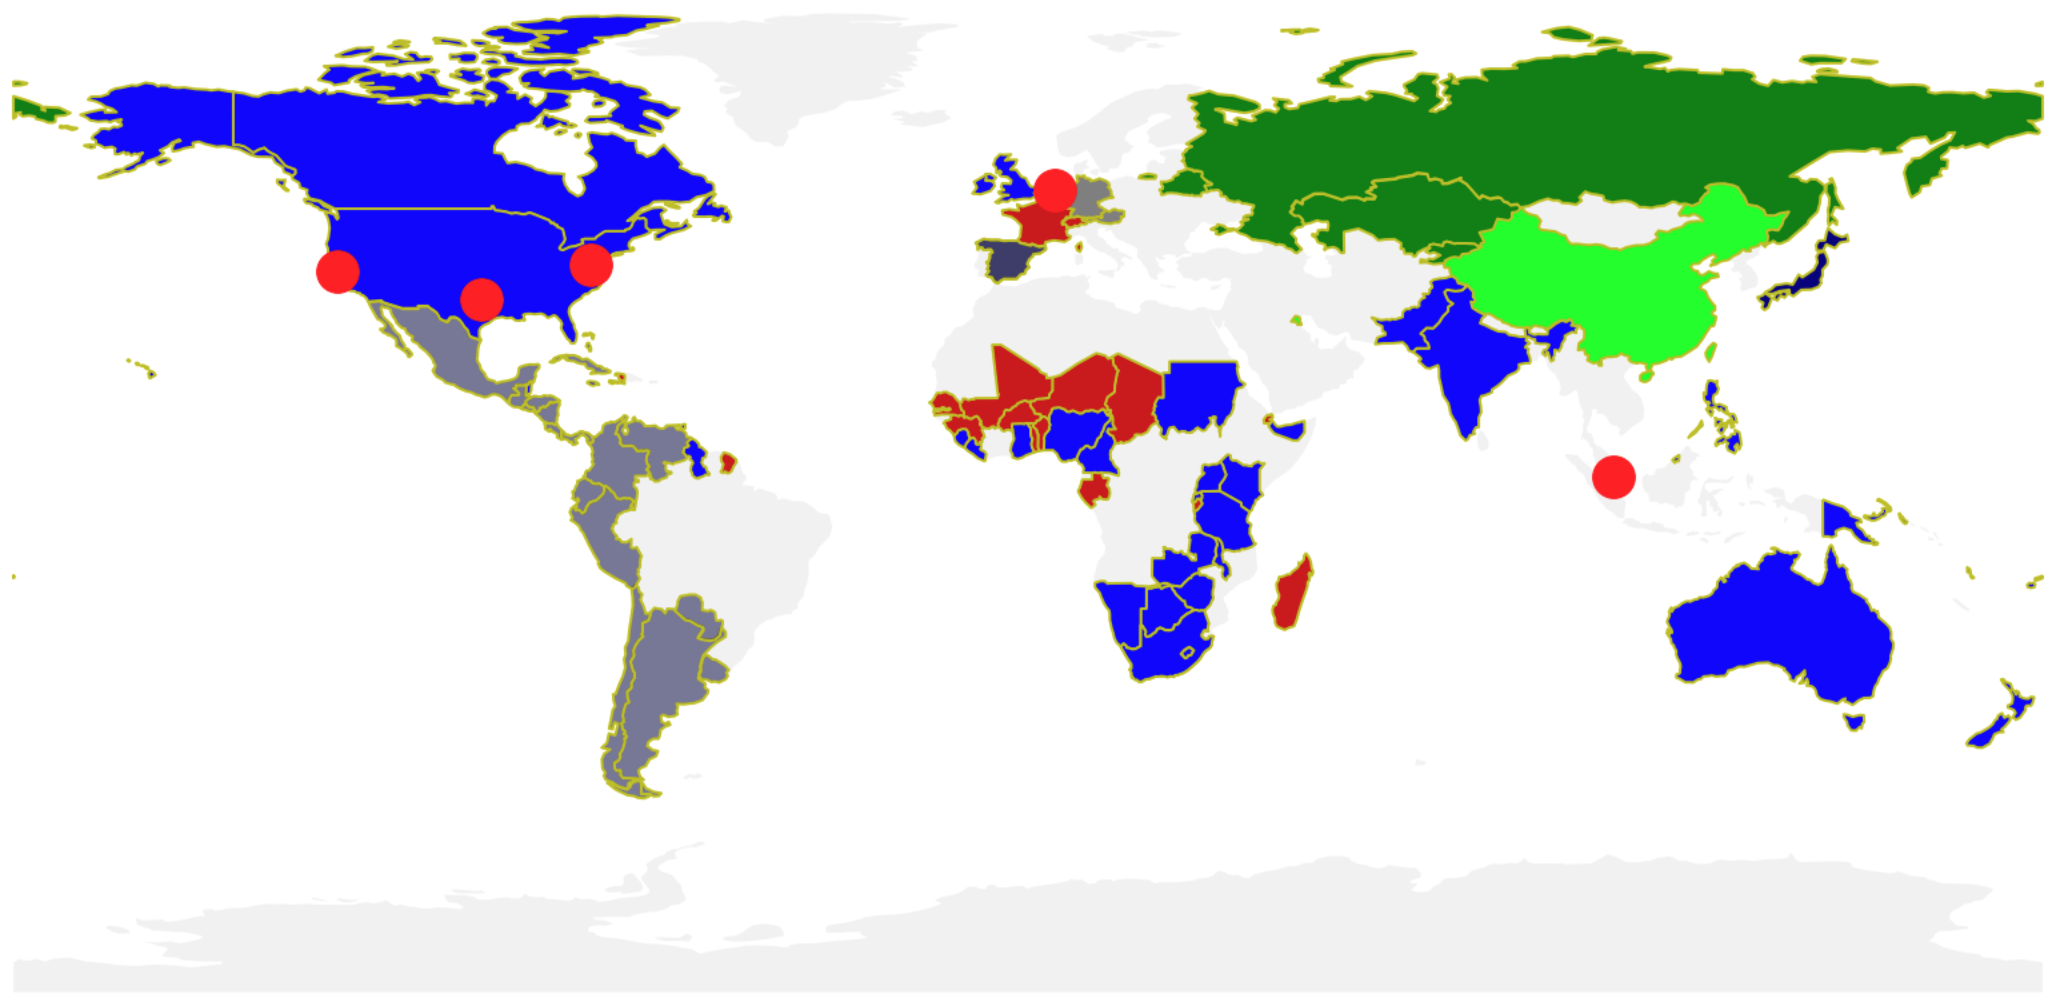
\includegraphics[width=1\textwidth]{embodied_cost_model/images/world_language_map_3.png}};
        \end{scope}
        
        \begin{scope}[xshift=1.0cm]
            \node [anchor=center] (chinese) at (2,-.6) {\small{Chinese}};
            \filldraw[outer color=chinese, inner color=chinese] (1.8,-.4) rectangle (2.2,0); % chinese
            
            \node [anchor=center] (english) at (4,-.6) {\small{English}};
            \filldraw[outer color=english, inner color=english] (3.8,-.4) rectangle (4.2,0); % english
            
            \node [anchor=center] (french) at (6,-.6) {\small{French}};
            \filldraw[outer color=french, inner color=french] (5.8,-.4) rectangle (6.2,0); % french
            
            \node [anchor=center] (german) at (8,-.6) {\small{German}};
            \filldraw[outer color=german, inner color=german] (7.8,-.4) rectangle (8.2,0); % german
            
            \node [anchor=center] (japanese) at (10,-.6) {\small{Japanese}};
            \filldraw[outer color=japanese, inner color=japanese] (9.8,-.4) rectangle (10.2,0); % japanese
            
            \node [anchor=center] (russian) at (12,-.6) {\small{Russian}};
            \filldraw[outer color=russian, inner color=russian] (11.8,-.4) rectangle (12.2,0); % russian
            
            \node [anchor=center] (spanish) at (14,-.6) {\small{Spanish}};
            \filldraw[outer color=spanish, inner color=spanish] (13.8,-.4) rectangle (14.2,0); % spanish
            
            \node [anchor=center] (dc_location) at (9,-1.1) {\small{Data Center Locations}};
            \filldraw[red] (7,-1.1) circle (4pt); 
            
            \end{scope}
            
        \end{tikzpicture}

\caption[Source country of language and DC locations]{Source country of language and DC locations map.}
\label{image:world_language_map}
\end{figure}
    
    Within these data center sites, specific sub-systems are segregated as listed in Table~\ref{tab:dc_subsystem_boundaries}. Demarcation by these sub-systems allows development of the embodied and operational models to align with industrial cost breakdown data and in terms of EIO industrial vectors. Table~\ref{tab:dc_subsystem_boundaries} serves the structural backbone for all the models developed in this framework as discussed next.
    
    \begin{table}[h]
\centering
\begin{tabular}{|l|l|} \hline
\bf{System Boundary} & \bf{Examples} \\ \hline 
Building Systems & Data Center Shell and Core \\ \hline
Cooling Systems & Air Handling Units and hydronic plants \\ \hline
Power Distribution & UPS, PDU, Cables, Diesel Generators \\ \hline
Information Technology & Compute, Storage, Network \\
\hline\end{tabular}
\caption{Sub System Boundaries}
\label{tab:dc_subsystem_boundaries}
\end{table}
    
    \subsection{Operational Inventories}
    
    \comment{The functional unit is not tied with the operational energy. The result maybe something like $\frac{kWh}{kw}$ (?) the lower the the number the more adverse it will be. Also this can be relative factor; i.e 1 for kWh*8760 hours, with kWh - kW capacity.}
    
    In this section, this research's methodology to assess the operational energy and carbon footprint of data center site infrastructure is presented. There are extensive theoretical data center energy use models in literature \cite{dayarathna16, joshi12}. These models can generally be segregated between IT and building systems domains. The model developed in this research couples the two domains by first selecting the the right IT component to model; i.e. the IT component that the total energy of the data centers is most sensitive to.
    
    Detailed industrial power usage insights are lacking in the public domain \cite{Masanet20}. As an exception some industrial insights are provided by Barroso in \cite{barroso18, barroso13}. Barroso provides Google's distribution of power for various points-of-use as indicted by the pie-charts shown in Figure~\ref{fig:power_dist_pies} for two generations of technology. In 2012, more than 80\% of the energy in a data center was used by four components; CPU 42\%, Cooling 15.4\%, disk 14.3\% and DRAM 11.7\%. By 2017, the cooling overhead had decreased to only account for 3\% a data center energy use, this decrease in cooling inflated the relative fraction of CPU and DRAM energy requirement. From these distributions, it is apparent that CPU's power usage is the dominant hot-spot.  
    
    \definecolor{pistachio}{rgb}{0.58, 0.77, 0.45} %cpu
\definecolor{denim}{rgb}{0.08, 0.38, 0.74} %dram
\definecolor{babyblue}{rgb}{0.54, 0.81, 0.94} % disk/hdd
\definecolor{azure}{rgb}{0.0, 0.5, 1.0} % storage
\definecolor{chartreuse}{rgb}{0.5, 1.0, 0.0} % nw
\definecolor{ashgrey}{rgb}{0.7, 0.75, 0.71} % balance/misc
\definecolor{bananamania}{rgb}{0.98, 0.91, 0.71} % psu
\definecolor{citrine}{rgb}{0.89, 0.82, 0.04} % power dist
\definecolor{cinnabar}{rgb}{0.89, 0.26, 0.2} %cooling

\begin{figure}[h]
\centering

\begin{tikzpicture}

% specify the pie charts
\node [anchor=center] (mix-ssd) at (0,3.5) {Power Allocation in 2012 \cite{barroso13}};
\pie[explode={0, 0, 0, 0}, , radius = 3, text=hide,color={pistachio, denim, babyblue, chartreuse, ashgrey, citrine, cinnabar }] 
{42/cpu, 11.7/dram, 14.3/disk, 4.9/nw, 4/misc, 7.7/power_dist, 15.4/cooling}
\definecolor{airforceblue}{rgb}{0.36, 0.54, 0.66}
\node [anchor=center] (mix-hdd) at (7,3.5) {Power Allocation in 2017 \cite{barroso18}};
\pie[pos={7,0}, explode = 0, radius = 3, text=hide, color={pistachio, denim, azure, chartreuse, ashgrey, citrine, cinnabar }] {60.6/cpu, 17.9/dram, 2.0/storage, 5.0/nw, 4/misc, 7.6/power_dist, 3.0/cooling}

%Specify the legend
\node [anchor=east] (cpu) at (-2,-3.8) {\small{CPU}};
\filldraw[outer color=pistachio, inner color=pistachio] (-2,-4) rectangle (-1.6,-3.6); % cpu

\node [anchor=east] (storage) at (0,-3.8) {\small{DRAM}};
\filldraw[outer color=denim, inner color=denim] (0,-4) rectangle (0.4,-3.6); % dram

\node [anchor=east] (disk) at (1.8,-3.8) {\small{Disk}};
\filldraw[outer color=babyblue, inner color=babyblue] (1.8,-4) rectangle (2.2,-3.6); % disk

\node [anchor=east] (psu) at (4,-3.8) {\small{Storage}};
\filldraw[outer color=azure, inner color=azure] (4,-4) rectangle (4.4,-3.6); %nw

\node [anchor=east] (balance) at (6.2,-3.8) {\small{Balance}};
\filldraw[outer color=ashgrey, inner color=ashgrey] (6.2,-4) rectangle (6.6,-3.6); % balance

\node [anchor=east] (power) at (10,-3.8) {\small{Power Distribution}};
\filldraw[outer color=citrine, inner color=citrine] (10,-4) rectangle (10.4,-3.6); % power dist

\node [anchor=east] (cooling) at (2,-4.6) {\small{Cooling}};
\filldraw[outer color=cinnabar, inner color=cinnabar] (2,-4.8) rectangle (2.4,-4.4); %cooling

\node [anchor=east] (nw) at (6,-4.6) {\small{Network}};
\filldraw[outer color=chartreuse, inner color=chartreuse] (6,-4.8) rectangle (6.4,-4.4); %nw

\end{tikzpicture}

\caption[Barroso's Power Distribution]{Data Center Power Distribution for Two Generation of Technology}
\label{fig:power_dist_pies}
\end{figure}
    
    The values in Figure~\ref{fig:power_dist_pies} are annualized distributions. In practice the power demand of data centers is very dynamic and sensitive to complex workload dependencies. These dependencies lend themselves to be exploited in power proportional computing paradigms. Several proportional workload techniques are discussed in detail by O'Sullivan in \cite{osullivan15}. This research takes such techniques and extends building energy models to be aware of proportional CPU loads based on coming network traffic to a data center site.
    
    Specifically, the embodied costs of the data center materials are extended to the EnergyPlus model from Chapter~\ref{chp:bem}. EnergyPlus provides a comprehensive indication of the operational energy and together with the marginal cost of energy model from Chapter~\ref{chp:mec}, it exposes the carbon footprint for each of the five data centers and the language abstracted service pairs. Both models are based on the network coefficients  from Chapter~\ref{chp:traffic}. The traffic coefficients are used to reset the IT workloads at each data centers and the marginal costs to produce energy in the regional grid. The details of the models is indicated in Algorithm~\ref{mec_coupled_bem_algo} and the general framework is illustrated in Figure~\ref{process_flow}.
    
      \begin{algorithm}

    \caption{MEC coupled BEM algorithm}
    \begin{algorithmic}
      \REQUIRE $DOSCOE[region_i]$ \& $traffic.language[site_{DC}]$
      \FOR{site and region in $DC.site$ and $DC.region$}
        \IF{traffic.language[site].all $!= 0$: }
        \STATE $D_{DC} \gets BEM(site, traffic.language[site_{DC}])$
        \STATE $DOSCOE[region].demand  \mathrel{+}=  D_{DC}$
        \ENDIF
      \ENDFOR
      \RETURN $CO_{2}$ {footprint}$\ =\ GridSim(region, rps)$
      
      \begin{small}
      \vspace{.1in}
      \STATE{\bf{Where}}: \\
     
        \hspace{.2in} $DOSCOE[region_i]$ = Dispatch Optimized System Cost of Energy Model for $region_i$ \cite{platt17}.  \\
        \hspace{.2in} $site_{DC}$ = data center site. \\
        \hspace{.2in} $traffic.language_l[site_{DC}]$ = the traffic routed to data center for lanuage $l$.  \\
        \hspace{.2in} $DC.site$ = list of all data centers in the network. \\
        \hspace{.2in} $DC.region$ = list of corresponding power grid region for the data centers in $DC.site$ . \\
        \hspace{.2in}$DOSCOE[region].demand$ = demand vector of loads added to the power grid for every hour. \\
        \vspace{.1in}
        \STATE{\bf{External Models}}: \\
        \vspace{.05in}
        \hspace{.2in}{$BEM(site, traffic.language[site_{DC}])$ is a EnergyPlus model of the data center. As an external argument the traffic profile for the language to the data center is passed. The traffic profiles serve as coefficients for the IT load, bounded by 0 and 1.  The output is a vector indicating the building energy demands for each hour of the year.} \\
        \vspace{.05in}
        \hspace{.2in}$GridSim(region, rps)$ is a DOSCOE model with $DOSCOE[region].demand$ and renewable portfolio standard ($rps$) value indicating the required penetration percentage of renewable energy in the power supply. The model quantifies the costs of energy in terms of carbon footprint and monetary values. 
        \end{small}
    \end{algorithmic}
    \label{mec_coupled_bem_algo}

  \end{algorithm}
    
    \begin{figure}[h]
\centering
\begin{tikzpicture}
% \node [anchor=west] (scope) at (8.75,5.5) {Embodied Costs};
\node [anchor=west] (embodied) at (9.6,-.3) {(Scope of Chapter)};
% \node [anchor=west] (traffic) at (1.4,5.5) {Traffic};
% \node [anchor=west] (bem) at (4.2,5.5) {BEM};
% \node [anchor=west] (mec) at (6.75,5.5) {MEC};
\begin{scope}[xshift=1.5cm]
    \node[anchor=south west,inner sep=0] (image) at (0,0) {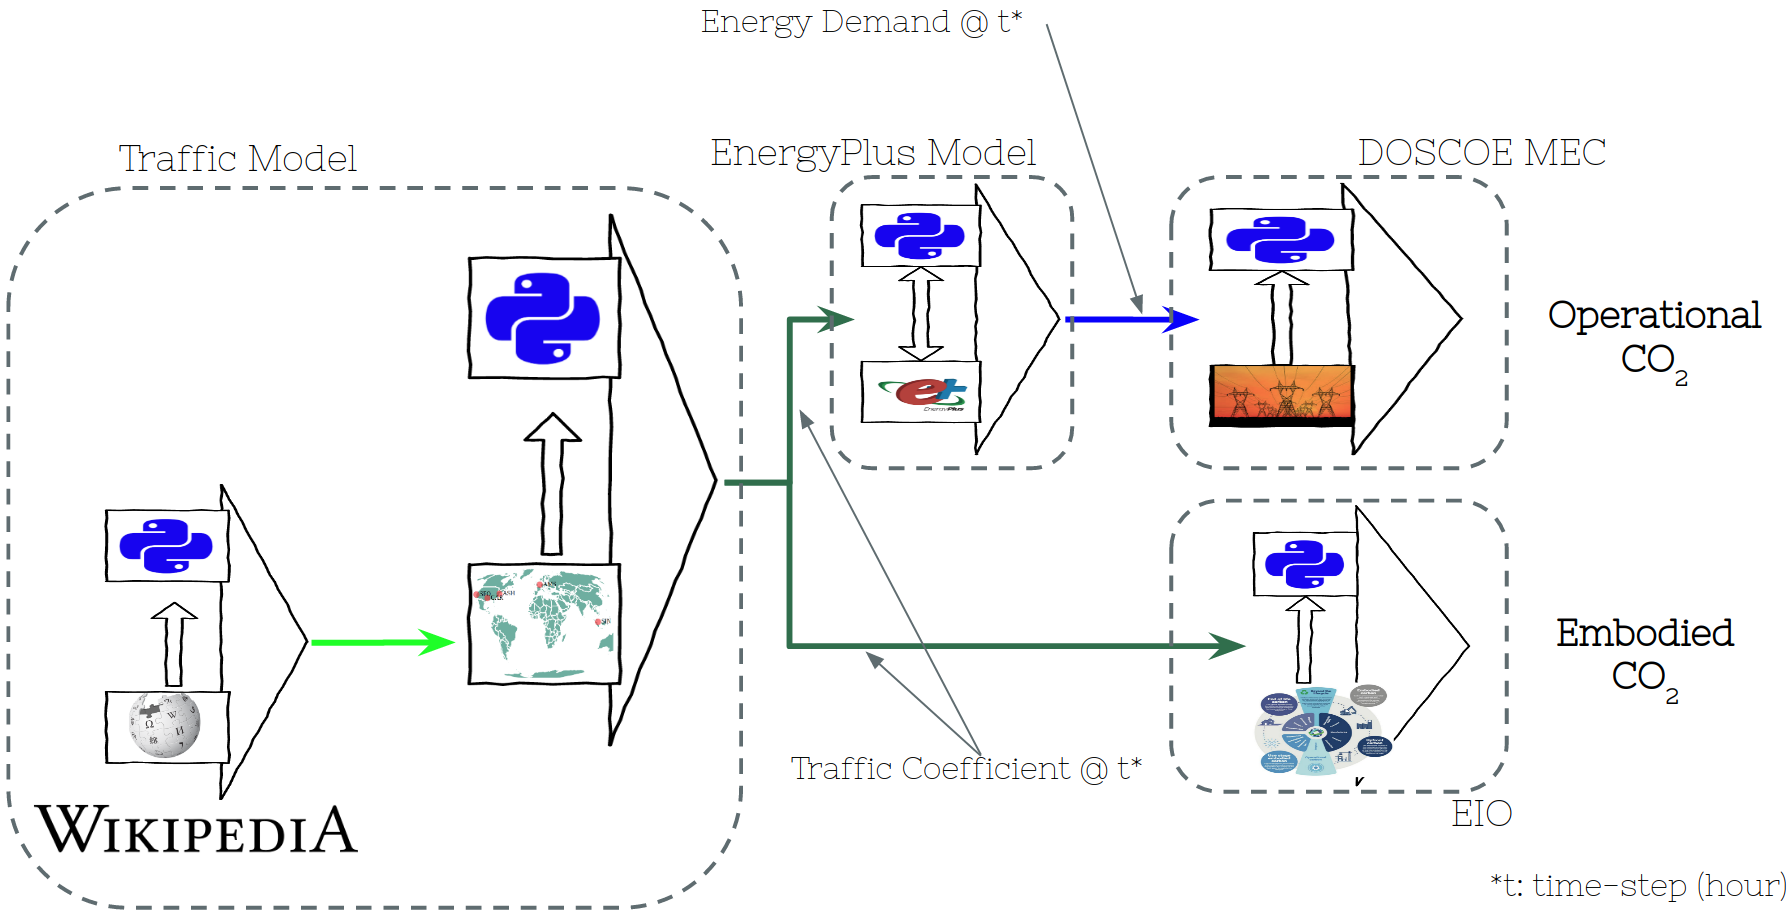
\includegraphics[width=0.8\textwidth]{embodied_cost_model/images/horizontal_process_flow2.png}};
    \begin{scope}[x={(image.south east)},y={(image.north west)}]
        \draw[ultra thick,rounded corners, ,dashed] (0.625,0.90) rectangle (1.05,0..08);
        % \draw [-stealth, line width=5pt, cyan] (scope) -- ++(0.6,0.0);
    \end{scope}
\end{scope}
\end{tikzpicture}
\caption[Model Process Flow Diagram]{Model Process Flow Diagram.}
\label{process_flow}
\end{figure}
    
    \subsection{Embodied Inventories}
    Embodied cost assessments account for the natural resources consumed when extracting, transforming, manufacturing, transporting, constructing, maintaining, and disposing the product under study. The first step in these assessments is to set the boundary conditions of the system. The second step is to select the method of the assessment. Two methods are available for such assessment; namely process based or EIO based. Process based methods are bottoms up procedures; accounting for all processes that are required to transform raw materials into consumer goods. However in process based methods as the product boundary and the count of processes to quantify can have exponentially correlations. This exponential growth can become an intractable task for building designers. A more tractable method is the EIO, where economic relationships between two industries at the national level are exploited. . 
    
    Leontief's original use case of the EIO was to identify the contribution from all economic sectors required to produce a unit of specific products in an economy.  The formulation of Leontief's EIO is indicated by Equation~\ref{eq:Leontief_IO}; where $Y$ is the input costs, $I$ is the identity matrix, and $A$ is the direct costs array \cite{matthews15}. In general direct costs represent the entire economy as a two-dimensional square array, where the rows and columns indicate distinct sectors within the economy. The values in the array indicate the row-index-sector’s input into the column-header-sector. Since their development in the 1930's, EIOs have been commonly used to characterize national economic accounts. More recently, Matthews and Hendrickson showed that EIO can be used for environmental life cycle assessments as-well \cite{matthews15}.  
    
        \begin{equation} \label{eq:Leontief_IO}
        [I-A]^{-1}Y
        \end{equation}
   
    Due to the streamlined approach of the EIO method compared to process based environmental assessments methods, the former is preferred for this research. Specifically, the United States Environmentally Extended Input-Out (USEEIO) model developed by Yang for the EPA is used in this research \cite{yang17}. The USEEIO’s economic relationship between sectors is based on 2007 cost data, while the environmental data are derived from 2013 emissions data. Both were the most up-to-date data available to the researchers at their time of publication. They suggest using 2013 cost of money for inputs, having demonstrated that the underlying structure of the economy has not shifted significantly between 2007 and 2013. 
    
        \subsubsection{Building Systems}
        Typically, data center shells and structural cores are under the jurisdiction of the same building codes as other commercial buildings, i.e. Type IIA construction types. However, the dense population of computers along with the  power and cooling requirements of data centers make several things clearly distinguishable from most commercial building types. The differences are significant enough to make the generic building sector's USEEIO environmental inventories invalid for data centers. 
        
        To more accurately represent data center buildings, several general contractor proposals for new data center construction and retrofit projects were reviewed for the cost distribution of the trades labor and equipment costs.  The contractor cost allocations per trade divisions were then compared with the values of the handful of building construction sectors available in the USEEIO. Based on the comparisons, the USEEIO manufacturing buildings sector is found to be the most similar for data centers. However, there are still shortfalls between data centers and the manufacturing buildings sector. To overcome the shortfalls, a hybrid method was used to construct a more representative Y vector for data centers. 
        
        The resulting Y vector for the building and building utilities systems is shown in Table~\ref{tab:eeio_y_building_table}. The table indicates the cost input required to provision a functional unit of 1 kW of data center capacity. Each sector's cost is derived from the contractor costs for the corresponding construction specification division as listed  in their proposals. Seven explicit sectors are quantified in addition to the manufacturing building sector. The manufacturing building/us is a catch all sector. This sector catches all the building trades that are not represented by the other entries in the Y vector; such as concrete or steel. 
        
        \begin{table}[h]
\centering
\begin{tabular}{|l|l|l|} \hline

\bf{ID} & \bf{Sector Name} & \bf{\$/kW}  \\ \hline

333415 & air conditioning, refrigeration, and heating equipment/us & 550 \\ \hline
333611 & turbines and turbine generator sets/us & 770 \\ \hline
335311 & specialty transformers/us & 50 \\ \hline
335313 & switchgear and switchboards/us & 100 \\ \hline
335920 & communication and energy wire and cable/us & 100 \\ \hline
335999 & other miscellaneous electrical equipment and components/us & 40 \\ \hline
335314 & relay and industrial controls/us & 150 \\ \hline
233230 & manufacturing buildings/us & 5250 \\ \hline

\end{tabular}
\caption{EEIO Costs Vector for Building and Utilities Infrastructure}
\label{tab:eeio_y_building_table}
\end{table}


        
        \subsubsection{Information Technology Systems}
        
        In this subsection the IT equipment's inventories are assessed. The IT equipment in a data center can be categorized broadly into three segments: compute, storage, and network. Within each of these segments, data center operators can further tune the hardware configurations to optimize their workloads. Figure~\ref{fig:server_cost_apportionment} indicates component wise cost distribution for five hardware stock-keeping units (SKU). The SKU data were obtained under non-disclosure agreements from a large internet website operator.  
        
        \definecolor{pistachio}{rgb}{0.58, 0.77, 0.45}
\definecolor{babyblue}{rgb}{0.54, 0.81, 0.94}
\definecolor{bananamania}{rgb}{0.98, 0.91, 0.71}
\definecolor{pinkpearl}{rgb}{0.91, 0.67, 0.81}
\definecolor{ashgrey}{rgb}{0.7, 0.75, 0.71}

\begin{figure}[h]
\centering

\begin{tikzpicture}
\node [anchor=center] (mix-ssd) at (0,1.75) {SSD Server};
\pie[explode={0, 0, 0, 0}, , radius = 1.5, text=hide,color={pistachio, babyblue, pinkpearl, bananamania, ashgrey}] {72/sc, 15/hdd, 5/mbd,
4/psu, 4/balance}

\node [anchor=center] (mix-hdd) at (4,1.75) {HDD Server};
\pie[pos={4,0}, explode = 0, radius = 1.5, text=hide, color={pistachio, babyblue, pinkpearl, bananamania, ashgrey}] {58/sc, 29/hdd, 6/mbd,
4/psu, 3/balance}

\node [anchor=center] (high-op) at (8,1.75) {High-IO Server};
\pie[pos={8,0}, explode = 0, radius = 1.5, text=hide, color={pistachio, babyblue, pinkpearl, bananamania, ashgrey}] {69/sc, 16/hdd, 7/mbd,
8/psu, 6/balance}

\node [anchor=center] (compute) at (2,-2.25) {Compute Server};
\pie[pos={2,-4}, explode = 0, radius = 1.5, text=hide, color={pistachio, babyblue, pinkpearl, bananamania, ashgrey}] {48/sc, 25/hdd, 13/mbd,
8/psu, 6/balance}

\node [anchor=center] (low-mem) at (6,-2.25) {Low-Memory Server};
\pie[pos={6,-4}, explode = 0, radius = 1.5, text=hide, color={pistachio, babyblue, pinkpearl, bananamania, ashgrey}] {51/sc, 34/hdd, 6/mbd,
4/psu, 5/balance}

\node [anchor=center] (semiconductor) at (.2,-7.25) {\small{CPU, Memory,}};
\node [anchor=center] (semiconductor) at (.2,-7.6) {\small{SSD}};
\node [anchor=center] (storage) at (2.7,-7.25) {\small{Hard Disc}};
\node [anchor=center] (storage) at (2.7,-7.6) {\small{Drive}};
\node [anchor=center] (pcb) at (5.2,-7.25) {\small{Motherboard}};
\node [anchor=center] (psu) at (7.7,-7.25) {\small{Power Supply}};
\node [anchor=center] (balance) at (10.2,-7.25) {\small{Balance}};

\filldraw[outer color=pistachio, inner color=pistachio] (0,-7) rectangle (0.4,-6.6);
\filldraw[outer color=babyblue, inner color=babyblue] (2.5,-7) rectangle (2.9,-6.6);
\filldraw[outer color=pinkpearl, inner color=pinkpearl] (5,-7) rectangle (5.4,-6.6);
\filldraw[outer color=bananamania, inner color=bananamania] (7.5,-7) rectangle (7.9,-6.6);
\filldraw[outer color=ashgrey, inner color=ashgrey] (10,-7) rectangle (10.4,-6.6);

\end{tikzpicture}

\caption[Server Cost Apportionment Chart]{Cost apportionment of deployable hardware. See Table~\ref{tab:sku_cost_dist_table} for details of USEEIO sector mapping. The values are representative of deployment cost share per server during 2015 and 2016. Data acquired by author from an DC operator under NDA.}
\label{fig:server_cost_apportionment}
\end{figure}
        
        The configuration of the server SKUs are optimized for the workloads that they support. For example the High-IO server is optimized for high rates of input and outputs; where it processes information at high feed rates. As an example, this useful for workloads that require external communications with a large data set that is housed in a Mix-SSD server that has an abundance of data storage capacity. For a data center with dominant heterogeneous workloads will have a mix of of these SKUs, whereas a data center with a single workload would have only one or two distinct SKUs.
        
        The values in Figure~\ref{fig:server_cost_apportionment} are indicative of the deployment cost share per server between 2015 and 2016. Server components such as processors (CPU), memory (MEM), and solid-state-drives (SSD) are fabricated using semiconductor manufacturing processes. These components are grouped together and are categorized as a single input into the USEEIO’s semiconductor sector. Hard disc drives (HDD), motherboard (MBD), and power supply units (PSU) have representative sectors that allow a one to one mapping within the USEEIO. Other components such as chassis, thermal-heat sinks, and cable connectors are grouped into the balance category. The balance category is mapped to the generic computer sector in USEEIO. This costs apportionment values can are used to construct the Y vector for input in the USEEIO.
        
        \newcommand*\rot{\rotatebox{90}}
\newcommand*\OK{\ding{51}}

\begin{table}[h]
\vspace{-10 pt}
\centering
\scalebox{0.8}{%
\begin{tabular}{|l|l|l|l|l|l|l|} \hline

\bf{Component} & \bf{USEEIO Sector} & \rot{\bf{SSD }} & \rot{\bf{Mix-HDD }} & \rot{\bf{High-IO }} & \rot{\bf{Compute}} & \rot{\bf{Low-Mem}} \\ \hline

CPU, Memory, & semiconductors/us & 72\% & 58\% & 69\% & 48\% & 51\% \\ 
SSD &  &  &  &  &  &  \\ \hline

HDD & computer storage & 15\% & 29\% & 16\% & 25\% & 34\% \\ 
 & device readers/us &  &  &  &  &  \\ \hline
 
Motherboard & printed circuit and  & 5\% & 6\% & 7\% & 13\% & 6\% \\
 & electronic assembly/us &  &  &  &  &  \\ \hline

Power Supply  & Electronic Capacitors & 4\% & 4\% & 4\% & 8\% & 4\% \\ 
Unit & and other components &  &  &  &  &  \\
 & (except semiconductors and &  &  &  &  &  \\ 
 & printed circuit assemblies)/us &  &  &  &  &  \\ \hline
 
Balance of Parts & computers/us & 3\% & 3\% & 3\% & 6\% & 4\% \\ \hline

\end{tabular}}
\caption{Cost apportionment of deployable hardware stock keeping units (SKU)}
\label{tab:sku_cost_dist_table}
\vspace{-10 pt}
\end{table}

        \begin{table}[h]
\vspace{-10 pt}
\centering
\begin{tabular}{|l|c|c|} \hline

\bf{Component} & \bf{Power (Watts)} & \bf{Reference} \\ \hline 

3.5" HDD & 3.87 & \cite{fuchs219} \\ \hline
2.5" HDD & 0.89 & \cite{fuchs219} \\ \hline
SDD & 0.37 & \cite{fuchs219} \\ \hline
Single Socket CPU & 105 & \cite{kaggle17b} \\ \hline
Dual Socket CPU & 210 & \cite{kaggle17b} \\ \hline
Power Supply Unit & 25 & \cite{joshi12} \\ \hline
Motherboards & 40 & \cite{buildcomputers} \\ \hline
RAM & 0.375 & \cite{crucial} \\ \hline
Fans (5 per server) & 10 & \cite{buildcomputers} \\ \hline


\hline\end{tabular}
\caption{Server component power distribution}
\label{tab:it_component_power_dist_table}
\vspace{-10 pt}
\end{table}
        
          \begin{algorithm}
    \caption{IT equipment Y vector algorithm}
    \begin{algorithmic}
      \REQUIRE $P_{DC}$, $P_{i}$, and $C_i$
      \STATE $P_{S} \gets \sum\limits_{i=1}^n P_{i}$
    %   \STATE $C_{S} \gets \sum\limits_{i=1}^n C_{i}$
      \STATE $C_{ip} \gets C_i \times f_i$
      \STATE $S_\# \gets \frac{P_{DC}}{P_{S}}$
      \STATE $SC_{DC} \gets S_\# \times P_{S}$
      
      \vspace{.1in}
      \RETURN $Y \gets SC_{DC} \times C_{ip}$
      
      \vspace{.1in}
      \STATE{\bf{Where}}: \\
        \hspace{.2in}$P_{DC}$ = Provisioned Power of Data Center, (input variable) \\
        \hspace{.2in}$P_{i}$ = Power demand for component $i$ of server.  \\
        \hspace{.2in}$n$ = Number of components in the server.  \\
        \hspace{.2in}$C_{ip}$ = Provisioning cost of component $i$ \\
        \hspace{.2in}$C_i$ = Cost Apportions for server component $i$, (from Figure~\ref{fig:server_cost_apportionment}) \\
        \hspace{.2in}$f_i$ = Failure rate of component $i$\\
        \hspace{.2in}$S_\#$ = Count of servers in data center \\
        \hspace{.2in}$SC_{DC}$ = Total Server Costs for DC \\
        \hspace{.2in}$Y$ = Vector of sector wise costs for input to USEEIO
    
    \end{algorithmic}
    \label{it_y_vector_algo}
  \end{algorithm}
        
        \begin{table}[h]
\centering
\begin{tabular}{|l|r|}

\hline
                                          \bf{Sector} & \bf{Direct} \\
\hline
\hline
\n                                334111/computers/us &    1.029522 \\
\n          334112/computer storage device readers/us &    0.146600 \\
\n                          420000/wholesale trade/us &    0.068705 \\
\n  33411a/computer terminals and other computer p... &    0.083782 \\
\n                           334413/semiconductors/us &    0.063247 \\
\n  334418/printed circuit and electronic assembly/us &    0.049135 \\
\n        550000/company and enterprise management/us &    0.018676 \\
\n  33441a/electronic capacitors, resistors, coils... &    0.011519 \\
\n         541800/advertising and public relations/us &    0.001979 \\
\n                          484000/truck transport/us &    0.006023 \\
\hline
\end{tabular}

\caption{Unit input to USEEIO computers/us sector}
\label{tab: generic_computer_eeio}

\end{table}
        


    
\section{Results}
\section{Discussions}
\section{Conclusion}
\newpage
\section{Appendix}
        
% \chapter{Life-Cycle Energy and Carbon Footprint Modeling with Data Center Building Energy Models}
\label{chp:embodied_cost_model}

\section{Introduction}
    In this chapter, the aim is to quantify the end to end life cycle costs of data centers by extending the operational models developed in the previous chapters. Those operational models have provided an indication of system level energy for a network of data centers and their marginal carbon dioxide footprints. Although, the presented models are a good proxy for the environmental costs of data center operations, they don't account for the energy and carbon footprint embodied in all the materials that the data centers are composed of.

    To assess the end to end environmental impact of data centers, this chapter describes a three-step hybrid life-cycle analysis inclusive of the embodied inventories of the physical data center infrastructure. As the first step, the building energy and marginal costs of energy generation models are reviewed. These two models together provide an indication of the respective costs during the operational phase of a data center's life. Then as the second step, a life cycle modeling framework using an economic input-output (EIO) analysis model extended to environmental costs is introduced. The inputs to the EIO are constructed in this chapter based on literature reviews and the researcher's industrial experience. The final step provides a global view of the end to end assessment by presenting the energy and carbon footprint of each of the data center-language pair analyzed in the previous chapters. With the global view, the global environmental costs of a discrete service can be assessed.

    \subsection{Motivations for an end to end life cycle cost model}
        In terms of scale, US data centers consumed 700 billion kWh in 2016. That was 1.8\% of the total electricity produced in the country according to a United States Department of Energy (DOE) report \cite{Shehabi16}. To drive further intuition of their scale, a typical 100-MW data center at peak load consumes the same amount of energy in an hour as 100 homes do in a month. Given a data centers power demands, it is not surprising that operational energy use has a high sensitivity towards their total cost of ownership (TCO); making it a key metric in TCO based design decisions. While optimization for use phase energy may significantly reduce the carbon footprint of a data center (given the source energy mix does not change), it does not account for other phases in the data center's end to end life cycle. Inventories from embodied life cycle phases such materialization, transit, maintenance, and end of life are left out of the operational phase energy models that have become prevalent indicator of data center sustainability. 

        There are two predominant paradigms for evaluating the embodied environmental inventories for any product that has been altered by technology (techno-sphere). The first method is process based. The complexity of a process-based model is greatly influenced by the boundary conditions of the study. If the boundary is demarcated between the biosphere and the techno-sphere, then the number of distinct life cycle processes to quantify explodes by 500 times for a simple pen \cite{shah11}. The alternate method is based on Leontief's macro-economic proxies that exploits economic correlations between industrial sectors. In macro-economic models, a matrix with rows and columns equal to the number of sectors in the economy is populated with the cost relationship between the row-sector and the corresponding column-sector. Industrial-sector macro-economic proxies reduce the problem space significantly as only one cost vector is required as input to analyze an entire economy. This research combines the two paradigms and presents a hybrid life-cycle assessment model of data centers that can be used to support data center design decisions. 

        The structure of the paper is as follows. First, some technical background about data centers is provided along with a synthesis of similar works. Then in the methodology section a dynamic model to quantify the operational and embodied costs of data center infrastructure is described. The results from the methods as then presented in the results section. This article concludes by summarizing its findings and suggesting the future direction in this area of research. 

\section{Background}
    \subsection{Technical Overview of Data Centers}
        Modern internet data centers are district scale systems, spanning campuses that are hundreds of acres. They may contain several hundred thousand pieces of information technology (IT) equipment. IT equipment consists of physical servers, network hardware nodes, and digital storage media. Theses pieces of IT equipment sit alongside the data center's district scale cooling and electrical distribution plants housed in warehouse-scale built environments. The environmental footprint of a data center spans the full breadth of these physical pieces of infrastructure. 

        At their scale data centers receive power through medium voltage connections with the local utility's grid. The alternating-current voltage may then be stepped down in several steps, but ultimately, it is rectified to be used by the sensitive electronic components in the information technology hardware. Each step-down is a point of power inefficiency, with the alternating-current to direct-current conversion being the biggest point of power loss. Furthermore, anywhere that the step down or conversion occurs inside the building, the electrical inefficiencies are manifested as heat.  

        The heat from the electrical inefficiencies, along with the heat emitted by the IT equipment transistor state transitions and their current leakage, must be rejected to the outside of the building space by mechanical means. At a fundamental level, a mechanically driven fluid mover is needed to convey the heat from indoors to outdoors or another reservoir. In single pass cooling systems fans intake outside-air and force them through the IT equipment, capturing any heat and carrying it outside of the buildings. More complex cooling systems may include liquid or gas refrigerant medium thermodynamic cycles between the buildings and reservoirs, with the refrigerant medium capturing heat at either the building room level or at the scale of IT equipment. Precise modeling of such data center building systems with intense therm-power dynamics is now a manageable task in building energy modeling software \cite{kumar20,kumar20b}. 

        The embodied costs of IT equipment and building systems yield additional environmental costs for a data center's life cycle. The rate of innovation for IT equipment and the ever-increasing demands from the software applications creates a capital market where TCO of one generation of IT hardware rapidly increases relative to newer IT hardware solutions. The capital of cost/performance trade-off makes the positive TCO life of IT equipment between two to five years as observed by Shehabi in the DOE report \cite{Shehabi16}. This relatively short lifetime of IT further compounds the embodied costs of data centers. For example, through a 20-year data center building life, four to ten generations of IT transit through the facility. Disparities in lifetimes and dimensional scale differences between buildings and microchips make data center embodied inventory modeling complex. However, recently hybrid life cycle assessment models have shown to be effective in quantifying the embodied costs of data centers \cite{shah11, whitehead15}. 

        Information technology equipment requires some further insights in order to make its impact to data center life cycle analysis more concrete and directed in scope. At the heart of information technology equipment are microprocessor chips. Modern chips are composed of billions of transistors which have been getting smaller in size since their first applications in electronics signal processing in the 1960's. Transistors have been the key enabler for the compaction and power efficiency gains of electronic devices over the years and they've also been shown to have one of the most dominant environmental costs within electronic products \cite{boyd09, alcaraz18}.

        Prior to the mid-2010's, transistors were composed of planar or 2-D architectures. 2-D transistors inherently had limited operational power efficiencies due to higher voltage and current leakage compared to the novel 3-D processors in the market today. Specifically it's the 3-D processes that have allowed significant operational efficiency gains for data centered operators, yet studies assessing the 3-D transistor architecture's impact to data center life cycle costs are lacking. The 2-D to 3-D transition is a recent example of rapid rate of adaption for information technology equipment that make generalized environmental impacts studies for transducer technology obsolete in two to three years \cite{murphy03}. The frequent churn of technology also drives rapid changes in the manufacturing process of the chips. These rapid changes in semiconductor-manufacturing processes necessitates a parametrically scalable framework where transistor chips can be evaluated in isolation from other server components.  

    \subsection{Similar Works}
        In this section similar works that have quantified the environmental foot print of data centers are presented. Data center life cycle assessment works come from industrial operators \cite{shah11},  academia \cite{whitehead15,kline16}, federal agencies \cite{CLEER13}, and industrial consortium's \cite{tgg12}. Two of the reviewed works are conducive to replicate from the ground up \cite{shah11,whitehead15}, while another serves as a guideline \cite{tgg12}, and another provides an online interactive tool to assess the footprint of targeted classes of Cloud services \cite{CLEER13}. 

        From the operators perspective Shah, demonstrates an end to end life cycle assessment of data center systems \cite{shah11}. Shah uses a hybrid model inclusive of process based and economic input/output assessment frameworks to assess a single a data center, while using a static model for use-phase power. Whitehead, extends Shah's hybrid work and demonstrates the life-cycle costs of a real data center and sets an explicit functional unit of 1-kW of provisioned capacity \cite{whitehead15}.  
        
        The recent focus on product operational energy efficiency motivated Kline’s study of the trade-offs between operational energy and the embodied costs of information technology equipment \cite{kline16}. Although their bases for the embodied costs are process based, their literature does not provide sufficient insight for others to reproduce the work. Similarly, The Green Grid's Data Center Life Cycle costs guidelines outline the end goal of a data center life cycle analysis. It classifies several key attributes that need to be considered, but lacks references to explicit procedures that must be followed to achieve the goals. 
        
       The Cloud Energy and Emissions Research (CLEER) Model provides a browser based user interface to compare the environmental costs of on-premise server based services with hypothetical cloud-based systems that would provide an equivalent service \cite{CLEER13}. CLEER's analysis is transparent and inclusive of embodied and operational costs, but it does not dynamically couple the embodied or operational costs into the model. The presented set of past works has inspired the methodology of this research as described in the next section.

\section{Methodology}
    \subsection{Functional Unit and Reference Flows}
    Life cycle assessment studies require a functional unit of performance of the system under study for use as a normalized reference point. As a reference point for data centers, there is an industry wide consensus that power is the best indicator for a data center's workload capacity \cite{shah11, whitehead15, barroso18}. Based on the consensus, the functional unit adapted for this research is chosen to be 1-kW of provisioned power per year. 
    
    Furthermore, for the abstracted functional unit to be used in comparisons between different data center design scenarios requires it to be translated to reference flow values. In this work the reference flow is constrained to 1-year of data center operations with the globally provisioned power footprint of each of the language abstracted internet services. The language (internet service) to data center distribution is indicated in Figure~\ref{land_dc_sankey}. 
    
    \begin{figure}[h!]\centering
    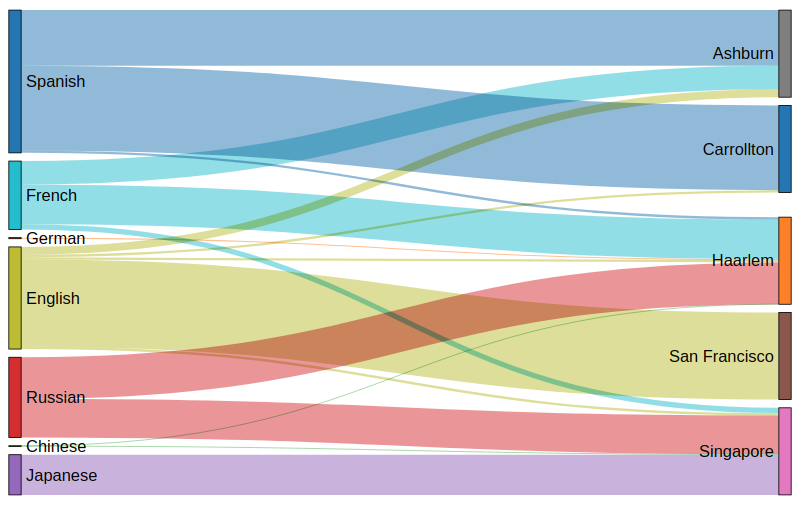
\includegraphics[scale=0.4]{embodied_cost_model/images/lang_dc_sankey.png}
    \caption[Language to Data Center Site Sankey Diagram]{Language to data center flows. The thickness of the links at each data center site indicate the relative portion of traffic that the respective language demands at the data center.}
    \label{land_dc_sankey}
    \end{figure}
    
    \subsection{System Boundary}
    The presented framework is intended to be used as a tool in data center life cycle assessments (LCA), where prevalent LCA practices are followed. In standard practice, product specific LCA studies generally entail four phases: 1) goal and scope phase, 2) the inventory analysis phase, 3) the impact assessment phase, and 4) the interpretation phase \cite{ISO14040}. The methodology, data sets, and software tools presented in the research is conducive for the first three LCA phases which all require quantitative assessment of data center environmental footprints. Stated more explicitly, this research’s goal is to provide a model that can be used to quantify the energy and carbon footprint of data center systems encompassing the embodied and operational phases in a single workflow. 
    
    Figure~\ref{system_boundary} illustrates the boundary conditions the boundary conditions with in the scope of this framework. In the scope are for paths of input of raw materials and energy from the ecosphere. Two paths lead to the embodied systems found in data centers; building construction and information technology manufacturing. While the other two path lead to the operational systems that are required to run the data centers. 
    
    \begin{figure}[h!]\centering
    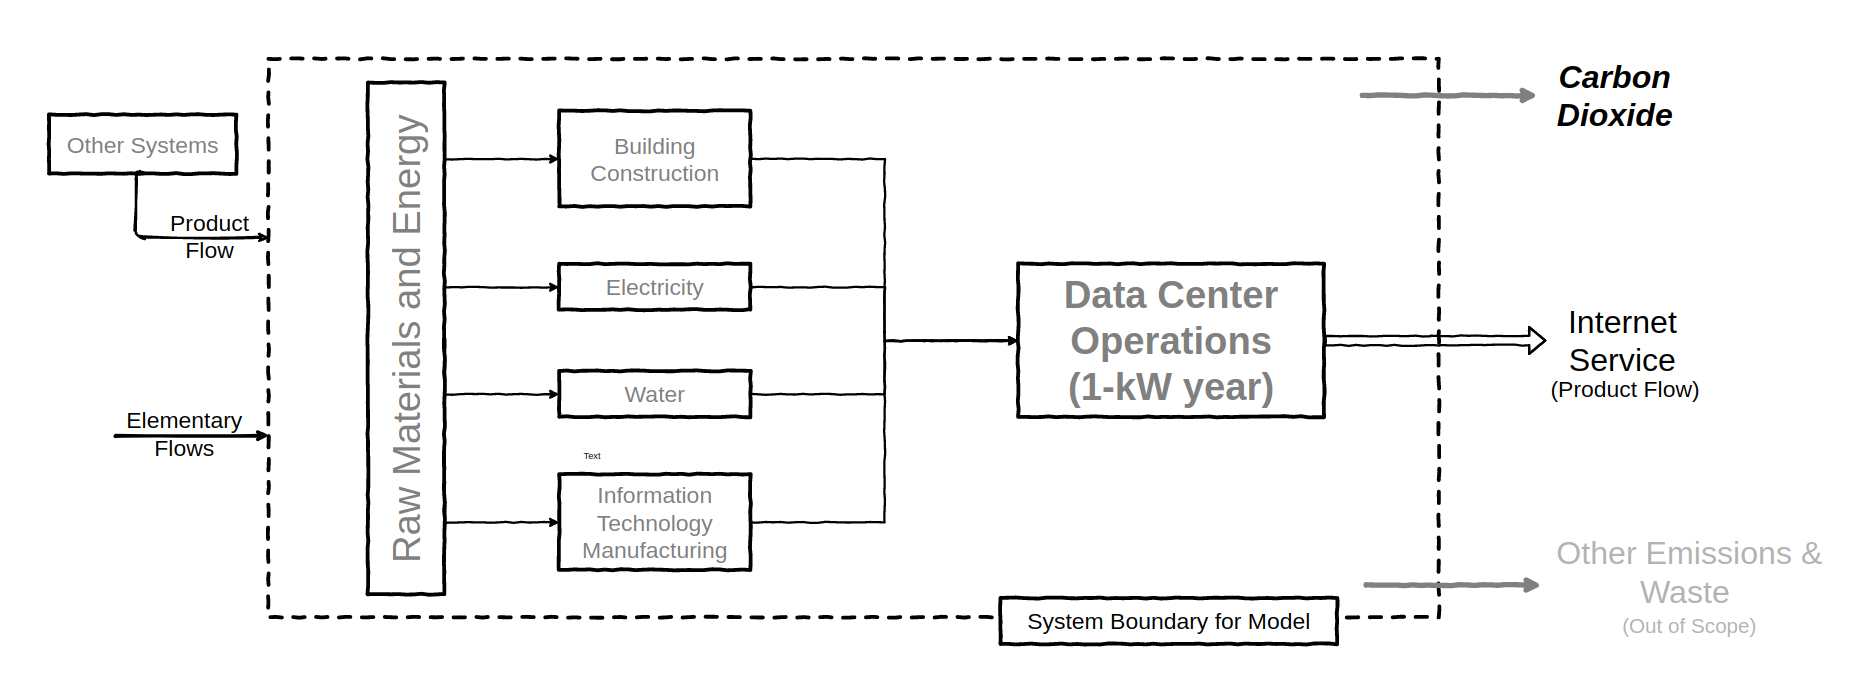
\includegraphics[scale=0.25]{embodied_cost_model/images/system_boundary2.png}
    \caption[System Boundary Diagram]{System Boundary for 1-kW of Provisioned Data Center Capacity.}
    \label{system_boundary}
    \end{figure}
    
    The geographical bounds of the service are illustrated in Figure~\ref{image:world_language_map}. The map indicates the countries in which each language from the Wikipedia set are the official languages. From  Figure~\ref{land_dc_sankey} it can be seen that one or more languages can be supported at a single data center facility. Although the workloads originate across international boundaries, the environmental emissions studied in this research are attributed to the data center sites only.  
    
    \definecolor{chinese}{rgb}{0, 1, 0} %chinese 
\definecolor{english}{rgb}{0, 0, 1}%english 
\definecolor{french}{rgb}{.8, 0, 0}%french 
\definecolor{german}{rgb}{.5, .5, .5}%german 
\definecolor{japanese}{rgb}{0, 0, .5}%japanese 
\definecolor{russian}{rgb}{0, .5, 0}%russian 
\definecolor{spanish}{rgb}{0, .25, .5}%spanish 


\begin{figure}[h]
\centering

        \begin{tikzpicture}
        \begin{scope}[xshift=1.5cm]
            \node[anchor=south west,inner sep=0] (image) at (0,0)
            {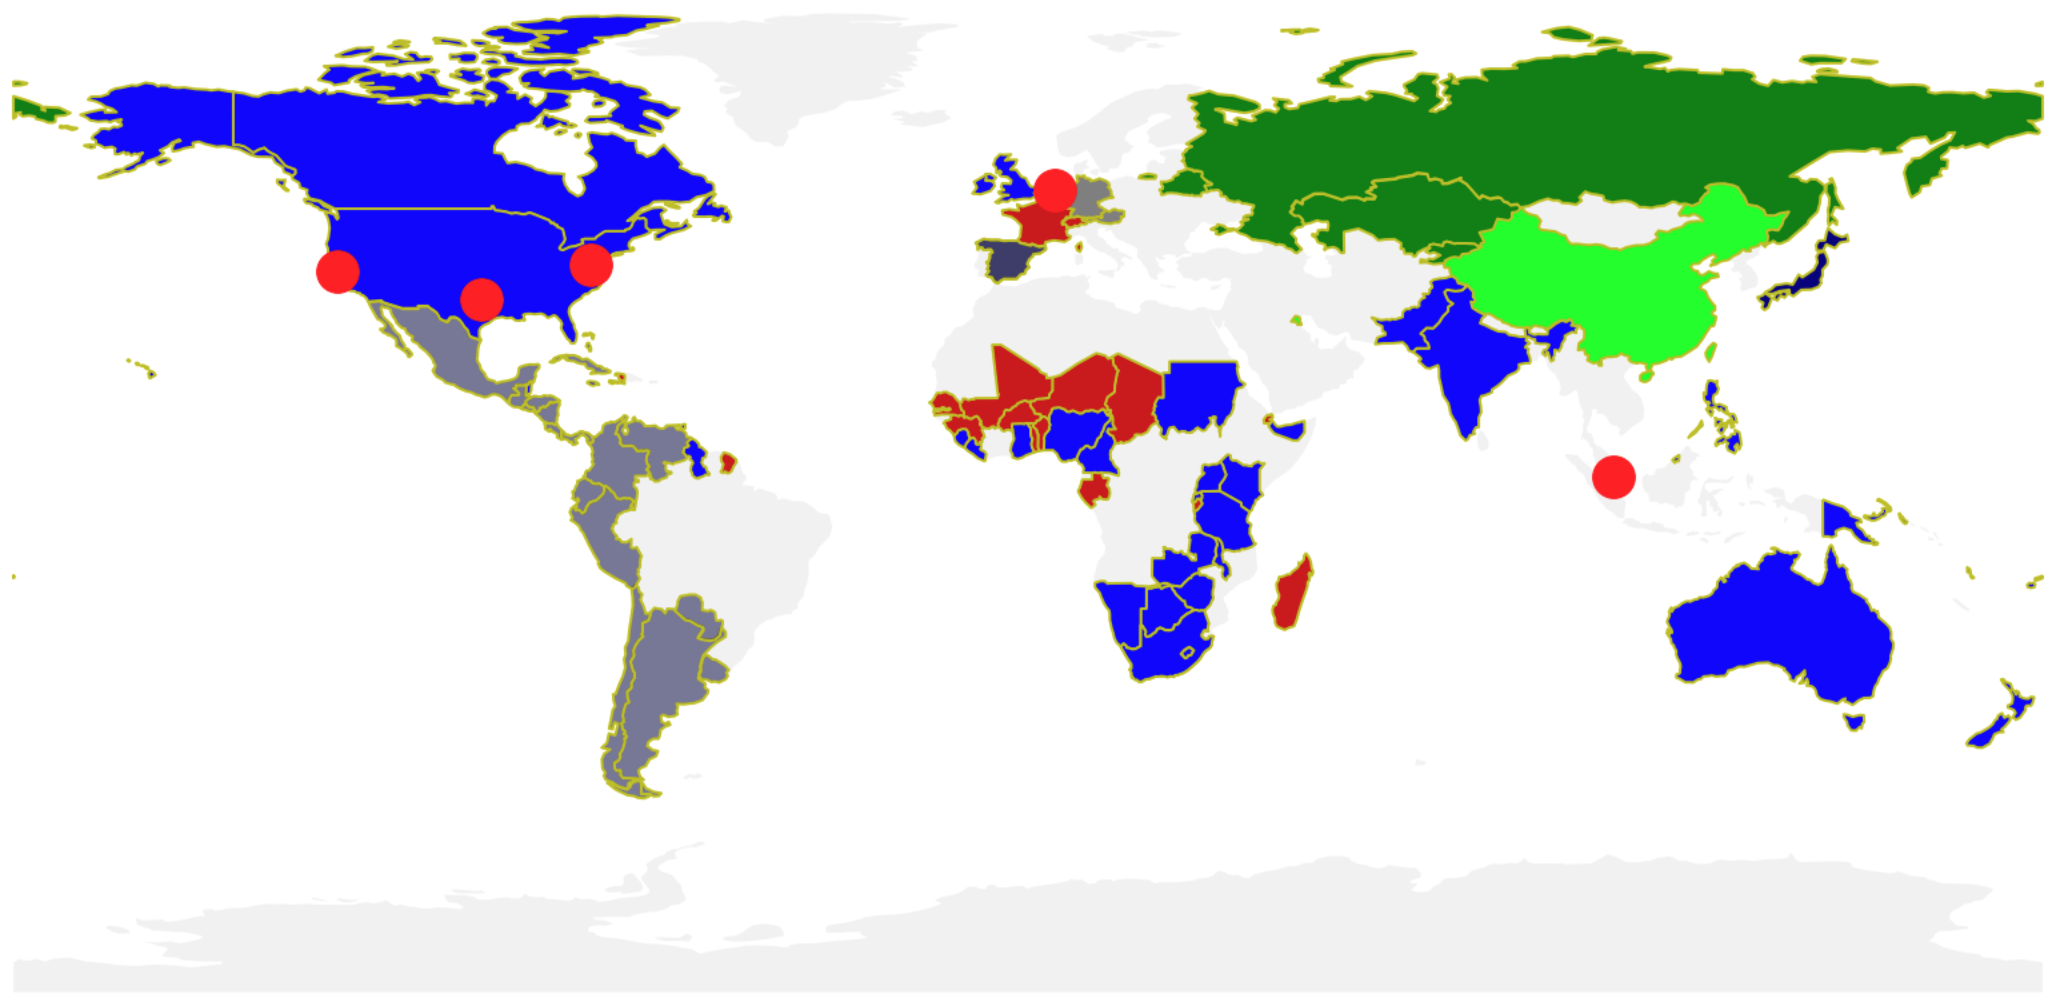
\includegraphics[width=1\textwidth]{embodied_cost_model/images/world_language_map_3.png}};
        \end{scope}
        
        \begin{scope}[xshift=1.0cm]
            \node [anchor=center] (chinese) at (2,-.6) {\small{Chinese}};
            \filldraw[outer color=chinese, inner color=chinese] (1.8,-.4) rectangle (2.2,0); % chinese
            
            \node [anchor=center] (english) at (4,-.6) {\small{English}};
            \filldraw[outer color=english, inner color=english] (3.8,-.4) rectangle (4.2,0); % english
            
            \node [anchor=center] (french) at (6,-.6) {\small{French}};
            \filldraw[outer color=french, inner color=french] (5.8,-.4) rectangle (6.2,0); % french
            
            \node [anchor=center] (german) at (8,-.6) {\small{German}};
            \filldraw[outer color=german, inner color=german] (7.8,-.4) rectangle (8.2,0); % german
            
            \node [anchor=center] (japanese) at (10,-.6) {\small{Japanese}};
            \filldraw[outer color=japanese, inner color=japanese] (9.8,-.4) rectangle (10.2,0); % japanese
            
            \node [anchor=center] (russian) at (12,-.6) {\small{Russian}};
            \filldraw[outer color=russian, inner color=russian] (11.8,-.4) rectangle (12.2,0); % russian
            
            \node [anchor=center] (spanish) at (14,-.6) {\small{Spanish}};
            \filldraw[outer color=spanish, inner color=spanish] (13.8,-.4) rectangle (14.2,0); % spanish
            
            \node [anchor=center] (dc_location) at (9,-1.1) {\small{Data Center Locations}};
            \filldraw[red] (7,-1.1) circle (4pt); 
            
            \end{scope}
            
        \end{tikzpicture}

\caption[Source country of language and DC locations]{Source country of language and DC locations map.}
\label{image:world_language_map}
\end{figure}
    
    Within these data center sites, specific sub-systems are segregated as listed in Table~\ref{tab:dc_subsystem_boundaries}. Demarcation by these sub-systems allows development of the embodied and operational models to align with industrial cost breakdown data and in terms of EIO industrial vectors. Table~\ref{tab:dc_subsystem_boundaries} serves the structural backbone for all the models developed in this framework as discussed next.
    
    \begin{table}[h]
\centering
\begin{tabular}{|l|l|} \hline
\bf{System Boundary} & \bf{Examples} \\ \hline 
Building Systems & Data Center Shell and Core \\ \hline
Cooling Systems & Air Handling Units and hydronic plants \\ \hline
Power Distribution & UPS, PDU, Cables, Diesel Generators \\ \hline
Information Technology & Compute, Storage, Network \\
\hline\end{tabular}
\caption{Sub System Boundaries}
\label{tab:dc_subsystem_boundaries}
\end{table}
    
    \subsection{Operational Inventories}
    
    \comment{The functional unit is not tied with the operational energy. The result maybe something like $\frac{kWh}{kw}$ (?) the lower the the number the more adverse it will be. Also this can be relative factor; i.e 1 for kWh*8760 hours, with kWh - kW capacity.}
    
    In this section, this research's methodology to assess the operational energy and carbon footprint of data center site infrastructure is presented. There are extensive theoretical data center energy use models in literature \cite{dayarathna16, joshi12}. These models can generally be segregated between IT and building systems domains. The model developed in this research couples the two domains by first selecting the the right IT component to model; i.e. the IT component that the total energy of the data centers is most sensitive to.
    
    Detailed industrial power usage insights are lacking in the public domain \cite{Masanet20}. As an exception some industrial insights are provided by Barroso in \cite{barroso18, barroso13}. Barroso provides Google's distribution of power for various points-of-use as indicted by the pie-charts shown in Figure~\ref{fig:power_dist_pies} for two generations of technology. In 2012, more than 80\% of the energy in a data center was used by four components; CPU 42\%, Cooling 15.4\%, disk 14.3\% and DRAM 11.7\%. By 2017, the cooling overhead had decreased to only account for 3\% a data center energy use, this decrease in cooling inflated the relative fraction of CPU and DRAM energy requirement. From these distributions, it is apparent that CPU's power usage is the dominant hot-spot.  
    
    \definecolor{pistachio}{rgb}{0.58, 0.77, 0.45} %cpu
\definecolor{denim}{rgb}{0.08, 0.38, 0.74} %dram
\definecolor{babyblue}{rgb}{0.54, 0.81, 0.94} % disk/hdd
\definecolor{azure}{rgb}{0.0, 0.5, 1.0} % storage
\definecolor{chartreuse}{rgb}{0.5, 1.0, 0.0} % nw
\definecolor{ashgrey}{rgb}{0.7, 0.75, 0.71} % balance/misc
\definecolor{bananamania}{rgb}{0.98, 0.91, 0.71} % psu
\definecolor{citrine}{rgb}{0.89, 0.82, 0.04} % power dist
\definecolor{cinnabar}{rgb}{0.89, 0.26, 0.2} %cooling

\begin{figure}[h]
\centering

\begin{tikzpicture}

% specify the pie charts
\node [anchor=center] (mix-ssd) at (0,3.5) {Power Allocation in 2012 \cite{barroso13}};
\pie[explode={0, 0, 0, 0}, , radius = 3, text=hide,color={pistachio, denim, babyblue, chartreuse, ashgrey, citrine, cinnabar }] 
{42/cpu, 11.7/dram, 14.3/disk, 4.9/nw, 4/misc, 7.7/power_dist, 15.4/cooling}
\definecolor{airforceblue}{rgb}{0.36, 0.54, 0.66}
\node [anchor=center] (mix-hdd) at (7,3.5) {Power Allocation in 2017 \cite{barroso18}};
\pie[pos={7,0}, explode = 0, radius = 3, text=hide, color={pistachio, denim, azure, chartreuse, ashgrey, citrine, cinnabar }] {60.6/cpu, 17.9/dram, 2.0/storage, 5.0/nw, 4/misc, 7.6/power_dist, 3.0/cooling}

%Specify the legend
\node [anchor=east] (cpu) at (-2,-3.8) {\small{CPU}};
\filldraw[outer color=pistachio, inner color=pistachio] (-2,-4) rectangle (-1.6,-3.6); % cpu

\node [anchor=east] (storage) at (0,-3.8) {\small{DRAM}};
\filldraw[outer color=denim, inner color=denim] (0,-4) rectangle (0.4,-3.6); % dram

\node [anchor=east] (disk) at (1.8,-3.8) {\small{Disk}};
\filldraw[outer color=babyblue, inner color=babyblue] (1.8,-4) rectangle (2.2,-3.6); % disk

\node [anchor=east] (psu) at (4,-3.8) {\small{Storage}};
\filldraw[outer color=azure, inner color=azure] (4,-4) rectangle (4.4,-3.6); %nw

\node [anchor=east] (balance) at (6.2,-3.8) {\small{Balance}};
\filldraw[outer color=ashgrey, inner color=ashgrey] (6.2,-4) rectangle (6.6,-3.6); % balance

\node [anchor=east] (power) at (10,-3.8) {\small{Power Distribution}};
\filldraw[outer color=citrine, inner color=citrine] (10,-4) rectangle (10.4,-3.6); % power dist

\node [anchor=east] (cooling) at (2,-4.6) {\small{Cooling}};
\filldraw[outer color=cinnabar, inner color=cinnabar] (2,-4.8) rectangle (2.4,-4.4); %cooling

\node [anchor=east] (nw) at (6,-4.6) {\small{Network}};
\filldraw[outer color=chartreuse, inner color=chartreuse] (6,-4.8) rectangle (6.4,-4.4); %nw

\end{tikzpicture}

\caption[Barroso's Power Distribution]{Data Center Power Distribution for Two Generation of Technology}
\label{fig:power_dist_pies}
\end{figure}
    
    The values in Figure~\ref{fig:power_dist_pies} are annualized distributions. In practice the power demand of data centers is very dynamic and sensitive to complex workload dependencies. These dependencies lend themselves to be exploited in power proportional computing paradigms. Several proportional workload techniques are discussed in detail by O'Sullivan in \cite{osullivan15}. This research takes such techniques and extends building energy models to be aware of proportional CPU loads based on coming network traffic to a data center site.
    
    Specifically, the embodied costs of the data center materials are extended to the EnergyPlus model from Chapter~\ref{chp:bem}. EnergyPlus provides a comprehensive indication of the operational energy and together with the marginal cost of energy model from Chapter~\ref{chp:mec}, it exposes the carbon footprint for each of the five data centers and the language abstracted service pairs. Both models are based on the network coefficients  from Chapter~\ref{chp:traffic}. The traffic coefficients are used to reset the IT workloads at each data centers and the marginal costs to produce energy in the regional grid. The details of the models is indicated in Algorithm~\ref{mec_coupled_bem_algo} and the general framework is illustrated in Figure~\ref{process_flow}.
    
      \begin{algorithm}

    \caption{MEC coupled BEM algorithm}
    \begin{algorithmic}
      \REQUIRE $DOSCOE[region_i]$ \& $traffic.language[site_{DC}]$
      \FOR{site and region in $DC.site$ and $DC.region$}
        \IF{traffic.language[site].all $!= 0$: }
        \STATE $D_{DC} \gets BEM(site, traffic.language[site_{DC}])$
        \STATE $DOSCOE[region].demand  \mathrel{+}=  D_{DC}$
        \ENDIF
      \ENDFOR
      \RETURN $CO_{2}$ {footprint}$\ =\ GridSim(region, rps)$
      
      \begin{small}
      \vspace{.1in}
      \STATE{\bf{Where}}: \\
     
        \hspace{.2in} $DOSCOE[region_i]$ = Dispatch Optimized System Cost of Energy Model for $region_i$ \cite{platt17}.  \\
        \hspace{.2in} $site_{DC}$ = data center site. \\
        \hspace{.2in} $traffic.language_l[site_{DC}]$ = the traffic routed to data center for lanuage $l$.  \\
        \hspace{.2in} $DC.site$ = list of all data centers in the network. \\
        \hspace{.2in} $DC.region$ = list of corresponding power grid region for the data centers in $DC.site$ . \\
        \hspace{.2in}$DOSCOE[region].demand$ = demand vector of loads added to the power grid for every hour. \\
        \vspace{.1in}
        \STATE{\bf{External Models}}: \\
        \vspace{.05in}
        \hspace{.2in}{$BEM(site, traffic.language[site_{DC}])$ is a EnergyPlus model of the data center. As an external argument the traffic profile for the language to the data center is passed. The traffic profiles serve as coefficients for the IT load, bounded by 0 and 1.  The output is a vector indicating the building energy demands for each hour of the year.} \\
        \vspace{.05in}
        \hspace{.2in}$GridSim(region, rps)$ is a DOSCOE model with $DOSCOE[region].demand$ and renewable portfolio standard ($rps$) value indicating the required penetration percentage of renewable energy in the power supply. The model quantifies the costs of energy in terms of carbon footprint and monetary values. 
        \end{small}
    \end{algorithmic}
    \label{mec_coupled_bem_algo}

  \end{algorithm}
    
    \begin{figure}[h]
\centering
\begin{tikzpicture}
% \node [anchor=west] (scope) at (8.75,5.5) {Embodied Costs};
\node [anchor=west] (embodied) at (9.6,-.3) {(Scope of Chapter)};
% \node [anchor=west] (traffic) at (1.4,5.5) {Traffic};
% \node [anchor=west] (bem) at (4.2,5.5) {BEM};
% \node [anchor=west] (mec) at (6.75,5.5) {MEC};
\begin{scope}[xshift=1.5cm]
    \node[anchor=south west,inner sep=0] (image) at (0,0) {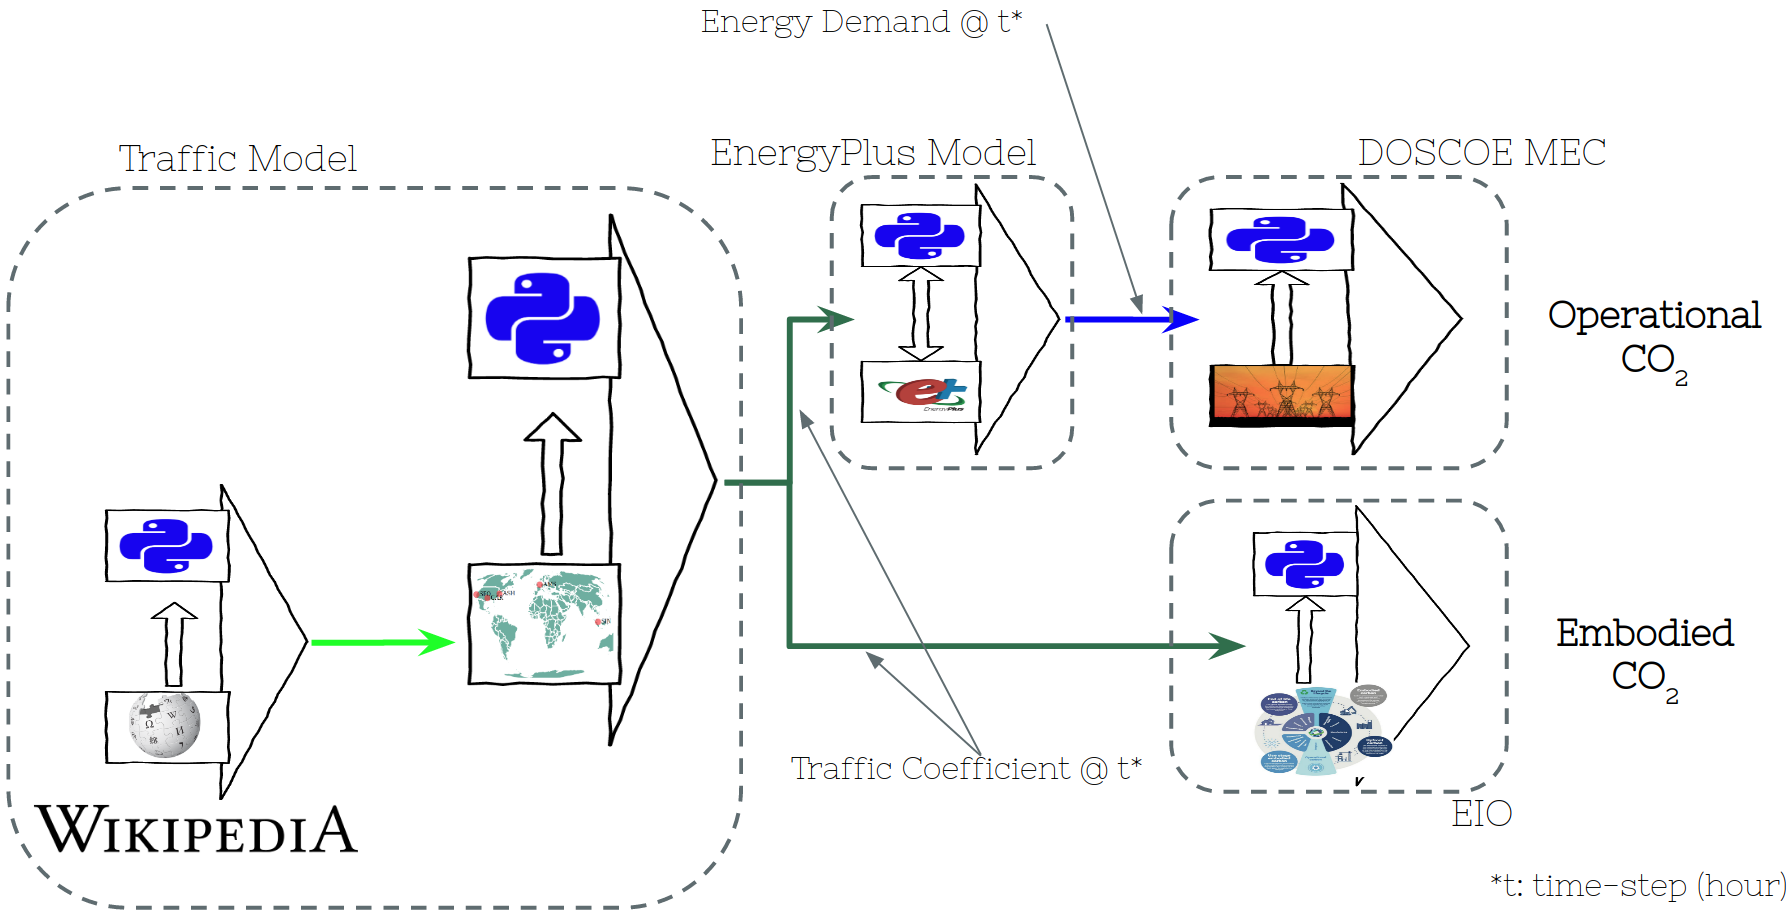
\includegraphics[width=0.8\textwidth]{embodied_cost_model/images/horizontal_process_flow2.png}};
    \begin{scope}[x={(image.south east)},y={(image.north west)}]
        \draw[ultra thick,rounded corners, ,dashed] (0.625,0.90) rectangle (1.05,0..08);
        % \draw [-stealth, line width=5pt, cyan] (scope) -- ++(0.6,0.0);
    \end{scope}
\end{scope}
\end{tikzpicture}
\caption[Model Process Flow Diagram]{Model Process Flow Diagram.}
\label{process_flow}
\end{figure}
    
    \subsection{Embodied Inventories}
    Embodied cost assessments account for the natural resources consumed when extracting, transforming, manufacturing, transporting, constructing, maintaining, and disposing the product under study. The first step in these assessments is to set the boundary conditions of the system. The second step is to select the method of the assessment. Two methods are available for such assessment; namely process based or EIO based. Process based methods are bottoms up procedures; accounting for all processes that are required to transform raw materials into consumer goods. However in process based methods as the product boundary and the count of processes to quantify can have exponentially correlations. This exponential growth can become an intractable task for building designers. A more tractable method is the EIO, where economic relationships between two industries at the national level are exploited. . 
    
    Leontief's original use case of the EIO was to identify the contribution from all economic sectors required to produce a unit of specific products in an economy.  The formulation of Leontief's EIO is indicated by Equation~\ref{eq:Leontief_IO}; where $Y$ is the input costs, $I$ is the identity matrix, and $A$ is the direct costs array \cite{matthews15}. In general direct costs represent the entire economy as a two-dimensional square array, where the rows and columns indicate distinct sectors within the economy. The values in the array indicate the row-index-sector’s input into the column-header-sector. Since their development in the 1930's, EIOs have been commonly used to characterize national economic accounts. More recently, Matthews and Hendrickson showed that EIO can be used for environmental life cycle assessments as-well \cite{matthews15}.  
    
        \begin{equation} \label{eq:Leontief_IO}
        [I-A]^{-1}Y
        \end{equation}
   
    Due to the streamlined approach of the EIO method compared to process based environmental assessments methods, the former is preferred for this research. Specifically, the United States Environmentally Extended Input-Out (USEEIO) model developed by Yang for the EPA is used in this research \cite{yang17}. The USEEIO’s economic relationship between sectors is based on 2007 cost data, while the environmental data are derived from 2013 emissions data. Both were the most up-to-date data available to the researchers at their time of publication. They suggest using 2013 cost of money for inputs, having demonstrated that the underlying structure of the economy has not shifted significantly between 2007 and 2013. 
    
        \subsubsection{Building Systems}
        Typically, data center shells and structural cores are under the jurisdiction of the same building codes as other commercial buildings, i.e. Type IIA construction types. However, the dense population of computers along with the  power and cooling requirements of data centers make several things clearly distinguishable from most commercial building types. The differences are significant enough to make the generic building sector's USEEIO environmental inventories invalid for data centers. 
        
        To more accurately represent data center buildings, several general contractor proposals for new data center construction and retrofit projects were reviewed for the cost distribution of the trades labor and equipment costs.  The contractor cost allocations per trade divisions were then compared with the values of the handful of building construction sectors available in the USEEIO. Based on the comparisons, the USEEIO manufacturing buildings sector is found to be the most similar for data centers. However, there are still shortfalls between data centers and the manufacturing buildings sector. To overcome the shortfalls, a hybrid method was used to construct a more representative Y vector for data centers. 
        
        The resulting Y vector for the building and building utilities systems is shown in Table~\ref{tab:eeio_y_building_table}. The table indicates the cost input required to provision a functional unit of 1 kW of data center capacity. Each sector's cost is derived from the contractor costs for the corresponding construction specification division as listed  in their proposals. Seven explicit sectors are quantified in addition to the manufacturing building sector. The manufacturing building/us is a catch all sector. This sector catches all the building trades that are not represented by the other entries in the Y vector; such as concrete or steel. 
        
        \begin{table}[h]
\centering
\begin{tabular}{|l|l|l|} \hline

\bf{ID} & \bf{Sector Name} & \bf{\$/kW}  \\ \hline

333415 & air conditioning, refrigeration, and heating equipment/us & 550 \\ \hline
333611 & turbines and turbine generator sets/us & 770 \\ \hline
335311 & specialty transformers/us & 50 \\ \hline
335313 & switchgear and switchboards/us & 100 \\ \hline
335920 & communication and energy wire and cable/us & 100 \\ \hline
335999 & other miscellaneous electrical equipment and components/us & 40 \\ \hline
335314 & relay and industrial controls/us & 150 \\ \hline
233230 & manufacturing buildings/us & 5250 \\ \hline

\end{tabular}
\caption{EEIO Costs Vector for Building and Utilities Infrastructure}
\label{tab:eeio_y_building_table}
\end{table}


        
        \subsubsection{Information Technology Systems}
        
        In this subsection the IT equipment's inventories are assessed. The IT equipment in a data center can be categorized broadly into three segments: compute, storage, and network. Within each of these segments, data center operators can further tune the hardware configurations to optimize their workloads. Figure~\ref{fig:server_cost_apportionment} indicates component wise cost distribution for five hardware stock-keeping units (SKU). The SKU data were obtained under non-disclosure agreements from a large internet website operator.  
        
        \definecolor{pistachio}{rgb}{0.58, 0.77, 0.45}
\definecolor{babyblue}{rgb}{0.54, 0.81, 0.94}
\definecolor{bananamania}{rgb}{0.98, 0.91, 0.71}
\definecolor{pinkpearl}{rgb}{0.91, 0.67, 0.81}
\definecolor{ashgrey}{rgb}{0.7, 0.75, 0.71}

\begin{figure}[h]
\centering

\begin{tikzpicture}
\node [anchor=center] (mix-ssd) at (0,1.75) {SSD Server};
\pie[explode={0, 0, 0, 0}, , radius = 1.5, text=hide,color={pistachio, babyblue, pinkpearl, bananamania, ashgrey}] {72/sc, 15/hdd, 5/mbd,
4/psu, 4/balance}

\node [anchor=center] (mix-hdd) at (4,1.75) {HDD Server};
\pie[pos={4,0}, explode = 0, radius = 1.5, text=hide, color={pistachio, babyblue, pinkpearl, bananamania, ashgrey}] {58/sc, 29/hdd, 6/mbd,
4/psu, 3/balance}

\node [anchor=center] (high-op) at (8,1.75) {High-IO Server};
\pie[pos={8,0}, explode = 0, radius = 1.5, text=hide, color={pistachio, babyblue, pinkpearl, bananamania, ashgrey}] {69/sc, 16/hdd, 7/mbd,
8/psu, 6/balance}

\node [anchor=center] (compute) at (2,-2.25) {Compute Server};
\pie[pos={2,-4}, explode = 0, radius = 1.5, text=hide, color={pistachio, babyblue, pinkpearl, bananamania, ashgrey}] {48/sc, 25/hdd, 13/mbd,
8/psu, 6/balance}

\node [anchor=center] (low-mem) at (6,-2.25) {Low-Memory Server};
\pie[pos={6,-4}, explode = 0, radius = 1.5, text=hide, color={pistachio, babyblue, pinkpearl, bananamania, ashgrey}] {51/sc, 34/hdd, 6/mbd,
4/psu, 5/balance}

\node [anchor=center] (semiconductor) at (.2,-7.25) {\small{CPU, Memory,}};
\node [anchor=center] (semiconductor) at (.2,-7.6) {\small{SSD}};
\node [anchor=center] (storage) at (2.7,-7.25) {\small{Hard Disc}};
\node [anchor=center] (storage) at (2.7,-7.6) {\small{Drive}};
\node [anchor=center] (pcb) at (5.2,-7.25) {\small{Motherboard}};
\node [anchor=center] (psu) at (7.7,-7.25) {\small{Power Supply}};
\node [anchor=center] (balance) at (10.2,-7.25) {\small{Balance}};

\filldraw[outer color=pistachio, inner color=pistachio] (0,-7) rectangle (0.4,-6.6);
\filldraw[outer color=babyblue, inner color=babyblue] (2.5,-7) rectangle (2.9,-6.6);
\filldraw[outer color=pinkpearl, inner color=pinkpearl] (5,-7) rectangle (5.4,-6.6);
\filldraw[outer color=bananamania, inner color=bananamania] (7.5,-7) rectangle (7.9,-6.6);
\filldraw[outer color=ashgrey, inner color=ashgrey] (10,-7) rectangle (10.4,-6.6);

\end{tikzpicture}

\caption[Server Cost Apportionment Chart]{Cost apportionment of deployable hardware. See Table~\ref{tab:sku_cost_dist_table} for details of USEEIO sector mapping. The values are representative of deployment cost share per server during 2015 and 2016. Data acquired by author from an DC operator under NDA.}
\label{fig:server_cost_apportionment}
\end{figure}
        
        The configuration of the server SKUs are optimized for the workloads that they support. For example the High-IO server is optimized for high rates of input and outputs; where it processes information at high feed rates. As an example, this useful for workloads that require external communications with a large data set that is housed in a Mix-SSD server that has an abundance of data storage capacity. For a data center with dominant heterogeneous workloads will have a mix of of these SKUs, whereas a data center with a single workload would have only one or two distinct SKUs.
        
        The values in Figure~\ref{fig:server_cost_apportionment} are indicative of the deployment cost share per server between 2015 and 2016. Server components such as processors (CPU), memory (MEM), and solid-state-drives (SSD) are fabricated using semiconductor manufacturing processes. These components are grouped together and are categorized as a single input into the USEEIO’s semiconductor sector. Hard disc drives (HDD), motherboard (MBD), and power supply units (PSU) have representative sectors that allow a one to one mapping within the USEEIO. Other components such as chassis, thermal-heat sinks, and cable connectors are grouped into the balance category. The balance category is mapped to the generic computer sector in USEEIO. This costs apportionment values can are used to construct the Y vector for input in the USEEIO.
        
        \newcommand*\rot{\rotatebox{90}}
\newcommand*\OK{\ding{51}}

\begin{table}[h]
\vspace{-10 pt}
\centering
\scalebox{0.8}{%
\begin{tabular}{|l|l|l|l|l|l|l|} \hline

\bf{Component} & \bf{USEEIO Sector} & \rot{\bf{SSD }} & \rot{\bf{Mix-HDD }} & \rot{\bf{High-IO }} & \rot{\bf{Compute}} & \rot{\bf{Low-Mem}} \\ \hline

CPU, Memory, & semiconductors/us & 72\% & 58\% & 69\% & 48\% & 51\% \\ 
SSD &  &  &  &  &  &  \\ \hline

HDD & computer storage & 15\% & 29\% & 16\% & 25\% & 34\% \\ 
 & device readers/us &  &  &  &  &  \\ \hline
 
Motherboard & printed circuit and  & 5\% & 6\% & 7\% & 13\% & 6\% \\
 & electronic assembly/us &  &  &  &  &  \\ \hline

Power Supply  & Electronic Capacitors & 4\% & 4\% & 4\% & 8\% & 4\% \\ 
Unit & and other components &  &  &  &  &  \\
 & (except semiconductors and &  &  &  &  &  \\ 
 & printed circuit assemblies)/us &  &  &  &  &  \\ \hline
 
Balance of Parts & computers/us & 3\% & 3\% & 3\% & 6\% & 4\% \\ \hline

\end{tabular}}
\caption{Cost apportionment of deployable hardware stock keeping units (SKU)}
\label{tab:sku_cost_dist_table}
\vspace{-10 pt}
\end{table}

        \begin{table}[h]
\vspace{-10 pt}
\centering
\begin{tabular}{|l|c|c|} \hline

\bf{Component} & \bf{Power (Watts)} & \bf{Reference} \\ \hline 

3.5" HDD & 3.87 & \cite{fuchs219} \\ \hline
2.5" HDD & 0.89 & \cite{fuchs219} \\ \hline
SDD & 0.37 & \cite{fuchs219} \\ \hline
Single Socket CPU & 105 & \cite{kaggle17b} \\ \hline
Dual Socket CPU & 210 & \cite{kaggle17b} \\ \hline
Power Supply Unit & 25 & \cite{joshi12} \\ \hline
Motherboards & 40 & \cite{buildcomputers} \\ \hline
RAM & 0.375 & \cite{crucial} \\ \hline
Fans (5 per server) & 10 & \cite{buildcomputers} \\ \hline


\hline\end{tabular}
\caption{Server component power distribution}
\label{tab:it_component_power_dist_table}
\vspace{-10 pt}
\end{table}
        
          \begin{algorithm}
    \caption{IT equipment Y vector algorithm}
    \begin{algorithmic}
      \REQUIRE $P_{DC}$, $P_{i}$, and $C_i$
      \STATE $P_{S} \gets \sum\limits_{i=1}^n P_{i}$
    %   \STATE $C_{S} \gets \sum\limits_{i=1}^n C_{i}$
      \STATE $C_{ip} \gets C_i \times f_i$
      \STATE $S_\# \gets \frac{P_{DC}}{P_{S}}$
      \STATE $SC_{DC} \gets S_\# \times P_{S}$
      
      \vspace{.1in}
      \RETURN $Y \gets SC_{DC} \times C_{ip}$
      
      \vspace{.1in}
      \STATE{\bf{Where}}: \\
        \hspace{.2in}$P_{DC}$ = Provisioned Power of Data Center, (input variable) \\
        \hspace{.2in}$P_{i}$ = Power demand for component $i$ of server.  \\
        \hspace{.2in}$n$ = Number of components in the server.  \\
        \hspace{.2in}$C_{ip}$ = Provisioning cost of component $i$ \\
        \hspace{.2in}$C_i$ = Cost Apportions for server component $i$, (from Figure~\ref{fig:server_cost_apportionment}) \\
        \hspace{.2in}$f_i$ = Failure rate of component $i$\\
        \hspace{.2in}$S_\#$ = Count of servers in data center \\
        \hspace{.2in}$SC_{DC}$ = Total Server Costs for DC \\
        \hspace{.2in}$Y$ = Vector of sector wise costs for input to USEEIO
    
    \end{algorithmic}
    \label{it_y_vector_algo}
  \end{algorithm}
        
        \begin{table}[h]
\centering
\begin{tabular}{|l|r|}

\hline
                                          \bf{Sector} & \bf{Direct} \\
\hline
\hline
\n                                334111/computers/us &    1.029522 \\
\n          334112/computer storage device readers/us &    0.146600 \\
\n                          420000/wholesale trade/us &    0.068705 \\
\n  33411a/computer terminals and other computer p... &    0.083782 \\
\n                           334413/semiconductors/us &    0.063247 \\
\n  334418/printed circuit and electronic assembly/us &    0.049135 \\
\n        550000/company and enterprise management/us &    0.018676 \\
\n  33441a/electronic capacitors, resistors, coils... &    0.011519 \\
\n         541800/advertising and public relations/us &    0.001979 \\
\n                          484000/truck transport/us &    0.006023 \\
\hline
\end{tabular}

\caption{Unit input to USEEIO computers/us sector}
\label{tab: generic_computer_eeio}

\end{table}
        


    
\section{Results}
\section{Discussions}
\section{Conclusion}
\newpage
\section{Appendix}
        


%> Page style for appendices. Do not modify.
\appendix\pagestyle{plain}

%> Appendices. If you have any appendices, put them here. Otherwise, remove these lines.
% \chapter{Experimental material}
\label{app:studyone}

\section{Participant solicitation for study one}
\label{app:studyone:solicitation}

Lorem ipsum dolor sit amet, consectetur adipiscing elit. Praesent porta faucibus magna. Duis volutpat odio at ante congue, vel interdum lorem ullamcorper. Proin placerat diam aliquam libero aliquet blandit. Curabitur sem sem, lacinia eget diam in, pretium lobortis ligula. Curabitur velit nunc, imperdiet vitae viverra id, sagittis sed sem. Nam cursus, ipsum in sollicitudin dapibus, massa dolor rutrum magna, eget tincidunt enim velit a est. Donec semper, lectus ac tincidunt varius, lacus est vestibulum quam, non convallis ligula justo id ipsum. Suspendisse cursus diam sed urna venenatis, a eleifend sem euismod.

Nullam nec tellus justo. Cras pulvinar, eros in aliquam mollis, metus massa ultrices quam, sit amet fermentum odio risus ac metus. Fusce malesuada gravida aliquet. Aliquam neque purus, interdum eget interdum ac, elementum eu magna. Nullam condimentum sem euismod auctor adipiscing. Aenean euismod mi ut imperdiet fringilla. Ut ac orci quis sem euismod posuere at luctus libero. Nullam vehicula ac diam ac ultrices.

\noindent Requisites to participate:
\begin{enumerate}
\item Vestibulum erat erat, mattis nec sem sit amet, pretium condimentum purus. 
\item Proin id tincidunt lorem, at vulputate erat.
\item In facilisis blandit arcu vitae laoreet. Curabitur consequat at metus ut feugiat.
\end{enumerate}

\section{Exit survey}
\label{app:studyone:gameform}

\begin{enumerate}[Q1.]
\item Donec nec dolor eget nisi faucibus scelerisque. Nulla facilisi. Vivamus accumsan quis orci eget auctor. Vestibulum ante ipsum primis in faucibus orci luctus et ultrices posuere cubilia Curae; Mauris facilisis nec risus et imperdiet. Nullam ac nibh arcu. Interdum et malesuada fames ac ante ipsum primis in faucibus. Mauris dictum urna lorem, id rutrum dolor aliquet nec. Sed ac nibh nec dolor luctus placerat. Nunc in justo id lorem iaculis elementum. Nullam feugiat viverra neque, non pulvinar nisl interdum id?

\item Nullam tempus bibendum felis, eget molestie quam imperdiet vitae. Vivamus diam orci, sollicitudin in facilisis eget, dictum lobortis sem. Vivamus quis purus massa. Fusce fermentum tempus leo, quis faucibus magna vehicula et. Donec ultricies neque et massa facilisis scelerisque. Etiam pulvinar velit pharetra massa vestibulum, vel vulputate lacus faucibus. Morbi imperdiet ante ut orci adipiscing, non adipiscing sapien congue. Ut imperdiet purus ipsum, vitae pellentesque magna volutpat vel?

\item Morbi placerat malesuada lectus a porttitor. Curabitur non ante cursus metus tempor convallis sodales nec leo. Etiam pretium lacus nec orci blandit, in fermentum turpis mattis. Duis tincidunt arcu non accumsan consectetur. Pellentesque non gravida mi. Aliquam fermentum felis eu nisl lobortis, ac sodales leo elementum. Donec sollicitudin nibh non gravida luctus. Fusce eget eros diam. Aenean et iaculis tellus?

\item Mauris luctus, erat nec consectetur interdum, lorem elit viverra augue, at sollicitudin arcu velit in ante. Donec ultrices risus turpis, non laoreet risus sodales nec. In aliquam tincidunt tincidunt. Sed non sem eu lorem lacinia fringilla id ac ipsum. Aenean aliquam pulvinar urna vel feugiat. Etiam eu lorem fermentum, iaculis nibh quis, ultrices velit. Phasellus et erat et risus rhoncus faucibus. In a sapien commodo, tempus justo sit amet, congue diam. Pellentesque risus dolor, laoreet vel laoreet ac, malesuada non sem. Aliquam cursus tellus in nibh ultrices ultricies. Donec ultrices mauris diam, id mollis diam vehicula quis. Nunc placerat at lorem at interdum. Etiam a euismod leo. Morbi enim nulla, lacinia quis metus id, fermentum tempus urna. Vestibulum nec posuere dui, ac ultricies nibh?

\item Etiam quis neque nec massa dapibus porta. Pellentesque nec elementum massa, vitae vulputate augue. Aliquam porttitor aliquam mauris, nec ultrices quam laoreet ac. Maecenas quis neque leo. Curabitur hendrerit sollicitudin justo, at pretium ipsum dictum vitae. Vestibulum cursus imperdiet felis. Aliquam vel enim vel leo feugiat faucibus at et leo?
\end{enumerate}
% \chapter{Difussion model}

Nulla varius diam turpis, nec consequat dolor semper ut. Suspendisse pellentesque, dui sed vulpu-
tate auctor, dolor magna aliquet lorem, sed pulvinar nisl turpis sed metus. Ut massa quam, cursus
et mollis quis, cursus vel justo. Interdum et malesuada fames ac ante ipsum primis in faucibus.
Proin sodales fringilla justo, quis bibendum felis ullamcorper in. Suspendisse congue, quam id
malesuada dignissim, purus dui hendrerit enim, et facilisis odio enim eu est. Donec at turpis quam.
Ut blandit diam ac sapien dignissim, non porttitor diam dictum. Donec eget massa gravida, iaculis
lorem eleifend, pellentesque quam.

\begin{displaymath}\sum_{i=0}^{\infty} x + 1\end{displaymath}

Proin eu auctor elit. Etiam tempor malesuada consequat. Mauris imperdiet purus ac erat
viverra, iaculis laoreet ligula molestie. Nunc ac justo augue. Morbi lorem nunc, condimentum non
lectus et, tempus accumsan quam. Vestibulum velit elit, mollis quis metus at, tempor consequat
massa.

\begin{equation}\sum_{i=0}^{\infty}x_i=\int_{0}^{\pi+2} f\end{equation}

\section{Proof}
Suppose on the contrary there exists a real number $L$ such that
\begin{displaymath}
\lim_{x\rightarrow\infty} \frac{f(x)}{g(x)} = L.
\end{displaymath}
Then
\begin{displaymath}
l=\lim_{x\rightarrow c} f(x)
= \lim_{x\rightarrow c}
\left[ g{x} \cdot \frac{f(x)}{g(x)} \right ]
= \lim_{x\rightarrow c} g(x) \cdot \lim_{x\rightarrow c}
\frac{f(x)}{g(x)} = 0\cdot L = 0,
\end{displaymath}
which contradicts our assumption that $l\neq 0$.


%> Bibliography style. Do not modify.
\bibliographystyle{IEEEtran}

%> If you come up with a different bibtex file, and don't want to change the name of the file,
%> you should change the name and location here (i.e., replace content/references for whatever
%> is your bib file). Otherwise, leave it as it is.
\bibliography{content/bibs}
\end{document}